
\chapter{Stress balance} \label{ssn_stress_balance}

\index{Balance equations!Stress}
In this chapter we decompose the state of stress with an ice-sheet into along-flow and across-flow components
\begin{align*}
  \rankone{\sigma}_n &= \ranktwo{\sigma} \cdot \hat{\rankone{u}}_n, \hspace{10mm}
  \rankone{\sigma}_t  = \ranktwo{\sigma} \cdot \hat{\rankone{u}}_t,
\end{align*}
where the unit-vectors $\hat{\rankone{u}}_n$ and $\hat{\rankone{u}}_t$ point in the direction of and tangential to the flow, respectively:
\begin{align}
  \label{flow_coordinate_system}
  \hat{\rankone{u}}_n &= \frac{[u\ v\ 0]\T}{\Vert \rankone{u}_h \Vert}, \hspace{5mm} \text{and} \hspace{5mm}
  \hat{\rankone{u}}_t  = \frac{[v\ \text{-}u\ 0]\T}{\Vert \rankone{u}_h \Vert},
\end{align}
where $\rankone{f}_h = [f_x\ f_y]\T$ denotes the horizontal components of the vector $\rankone{f}$.

\section{Membrane stress} \label{ssn_membrane_stress}

\index{Membrane stress}
Let coordinates $(i,j,z)$ be the transformed velocity-coordinate system in the direction of flow, tangential to flow, and in the positive vertical direction, respectively.  The unit vectors of this rotated coordinate system are
\begin{align}
  \label{flow_coordinate_vectors}
  \hat{\rankone{u}} = [\hat{u}\ \hat{v}\ 0]\T \hspace{5mm} 
  \hat{\rankone{v}} = [\hat{v}\ \text{-}\hat{u}\ 0]\T \hspace{5mm}
  \hat{\rankone{w}} = [0\ 0\ \hat{w}]\T,
\end{align}
with normalized velocity vector components
\begin{align}
  \label{normalized_velocity_components}
  \hat{u} = \frac{u}{\Vert \rankone{u}_h \Vert}, \hspace{8mm}
  \hat{v} = \frac{v}{\Vert \rankone{u}_h \Vert}, \hspace{8mm}
  \hat{w} = 1.
\end{align}
The partial derivatives in this new coordinate system can be evaluated using the directional derivatives \index{Directional derivative}
\begin{align*}
  \parder{f}{i} &= \nabla_{\hat{\rankone{u}}} f = \nabla f \cdot \hat{\rankone{u}} = \parder{f}{x} \hat{u} + \parder{f}{y} \hat{v} \\
  \parder{f}{j} &= \nabla_{\hat{\rankone{v}}} f = \nabla f \cdot \hat{\rankone{v}} = \parder{f}{x} \hat{v} - \parder{f}{y} \hat{u} \\
  \parder{f}{z} &= \nabla_{\hat{\rankone{w}}} f = \nabla f \cdot \hat{\rankone{w}} = \parder{f}{z},
\end{align*} 
and the $z$-rotated gradient operator
\begin{align}
  \label{transformed_gradient_operator}
  \nabla_r \equiv \left[ \parder{}{i}\ \parder{}{j}\ \parder{}{z} \right]\T.
\end{align}

Next, let $\phi$ be the signed angle in radians between the $x$-axis and the horizontal velocity vector $\rankone{u}_h = [u\ v]\T$.  The rotation matrix about the $z$-axis used to transform any vector in the $x$, $y$, $z$ coordinate system to the $i$, $j$, $z$ coordinate system is
\begin{align*}
  \ranktwo{R}_z &= \begin{bmatrix}[c]
                     \cos(\phi)  & -\sin(\phi) & 0 \\
                     \sin(\phi)  &  \cos(\phi) & 0 \\
                     0           &  0          & 1
                   \end{bmatrix},
\end{align*}
and the $\phi$-rotation of the rank-two Cauchy-stress tensor $\ranktwo{\sigma}$ about the $z$-axis is
\begin{align}
  \label{rotated_stress_tensor}
  \ranktwo{\sigma}_r = \ranktwo{R}_z \cdot \ranktwo{\sigma} \cdot \ranktwo{R}_z\T
                     = \begin{bmatrix}
                         \sigma_{ii} & \sigma_{ij} & \sigma_{iz} \\
                         \sigma_{ji} & \sigma_{jj} & \sigma_{jz} \\
                         \sigma_{zi} & \sigma_{zj} & \sigma_{zz}
                       \end{bmatrix}.
\end{align}

Returning to momentum balance (\ref{cons_momentum}), the $\phi$-rotated momentum balance is
\begin{align}
  \label{rotated_momentum_balance}
  - \nabla_r \cdot \ranktwo{\sigma}_r &= \rankone{f},
\end{align}
leading to an expansion similar to (\ref{stokes_exp}),
\begin{align*}
  \parder{\sigma_{ii}}{i} + \parder{\sigma_{ij}}{j} + \parder{\sigma_{iz}}{z} &= 0 \\ 
  \parder{\sigma_{ji}}{i} + \parder{\sigma_{jj}}{j} + \parder{\sigma_{jz}}{z} &= 0 \\ 
  \parder{\sigma_{zi}}{i} + \parder{\sigma_{zj}}{j} + \parder{\sigma_{zz}}{z} &= \rho g.
\end{align*}

Next, rotated momentum-balance (\ref{rotated_momentum_balance}) is integrated vertically, 
\begin{align}
  \label{vertically_integrated_stress_balance_one}
  - \int_B^S \nabla_r \cdot \ranktwo{\sigma}_r \d{z} &= \int_B^S \rankone{f} \d{z}.
\end{align}
Similar to the derivation of vertically-integrated mass-balance (\ref{integrated_cons_mass}), Leibniz's rule (\ref{leibniz_rule}) \index{Leibniz's rule!Stress balance} is applied to the above, resulting in the vertically-integrated stress-balance
\begin{align}
  \label{vertically_integrated_stress_balance}
  - \nabla_r \cdot \left( \int_B^S \ranktwo{\sigma}_r \d{z} \right) + \ranktwo{\sigma}_r |_S \cdot \nabla_r S - \ranktwo{\sigma}_r |_B \cdot \nabla_r B &= \int_B^S \rankone{f} \d{z}.
\end{align}

It is also of interest to examine the state of stress without the contribution of the mean compressive stress $p = -\sigma_{kk} / 3$,  and thus perform a similar set of calculations as above to deviatoric stress-tensor $\ranktwo{\tau}$ in Cauchy stress tensor (\ref{stress_tensor}).  The rotated-stress-deviator tensor is thus
\begin{align}
  \label{rotated_stress_deviator_tensor}
  \ranktwo{\tau}_r = \ranktwo{R}_z \cdot \ranktwo{\tau} \cdot \ranktwo{R}_z\T
         = \begin{bmatrix}
             \tau_{ii} & \tau_{ij} & \tau_{iz} \\
             \tau_{ji} & \tau_{jj} & \tau_{jz} \\
             \tau_{zi} & \tau_{zj} & \tau_{zz}
           \end{bmatrix},
\end{align}
such that stress tensor (\ref{rotated_stress_tensor}) may be decomposed using Cauchy stress (\ref{stress_tensor}) into
\begin{align*}
  \ranktwo{\sigma}_r = \ranktwo{\tau}_r - p \ranktwo{I}
           = \begin{bmatrix}
               \tau_{ii} & \tau_{ij} & \tau_{iz} \\
               \tau_{ji} & \tau_{jj} & \tau_{jz} \\
               \tau_{zi} & \tau_{zj} & \tau_{zz}
             \end{bmatrix} - 
           p \begin{bmatrix}
               1 & 0 & 0 \\
               0 & 1 & 0 \\
               0 & 0 & 1 
             \end{bmatrix}.
\end{align*}
Therefore, using the fact that $\nabla_r \cdot \big(p \ranktwo{I} \big) = \nabla_r p$, vertically-integrated stress-balance (\ref{vertically_integrated_stress_balance}) may also be written
{\footnotesize
\begin{align}
  \label{vertically_integrated_stress_balance_decomposed}
  - \nabla_r \cdot \left( \int_B^S \ranktwo{\tau}_r \d{z} \right) + \ranktwo{\tau}_r |_S \cdot \nabla_r S - \ranktwo{\tau}_r |_B \cdot \nabla_r B &= \int_B^S \left( \rankone{f} - \nabla_r p \right) \d{z}.
\end{align}}

Finally, the terms of the vertically-integrated deviatoric-stress tensor $\int_z \ranktwo{\tau}_r \d{z} = \ranktwo{N}$ contains individual components \index{Tensor!Membrane stress}
\begin{align}
  \label{membrane_stress_tensor}
  \ranktwo{N} &= \begin{bmatrix}
                   N_{ii} & N_{ij} & N_{iz} \\
                   N_{ji} & N_{jj} & N_{jz} \\
                   N_{zi} & N_{zj} & N_{zz}
                 \end{bmatrix}
               = \begin{bmatrix}
                   \int_z \tau_{ii} & \int_z \tau_{ij} & \int_z \tau_{iz}  \\ 
                   \int_z \tau_{ji} & \int_z \tau_{jj} & \int_z \tau_{jz}  \\ 
                   \int_z \tau_{zi} & \int_z \tau_{zj} & \int_z \tau_{zz}
                 \end{bmatrix},
\end{align}
and are referred to as \emph{membrane stresses} \citep{greve_2009}.  

\section{Membrane stress balance} \label{ssn_membrane_stress_balance}

Re-writing stress balance (\ref{vertically_integrated_stress_balance_one}) using (\ref{vertically_integrated_stress_balance_decomposed}), we have an equivalent form of (\ref{vertically_integrated_stress_balance_decomposed}), the \emph{membrane stress balance}
\begin{align}
  \label{membrane_stress_balance}
  - \ranktwo{M} \rankone{1} = \rankone{f}_{\text{int}}, 
\end{align}
where $\rankone{1} = [1\ 1\ 1]\T$ is the rank-one tensor of ones, $\rankone{f}_{\text{int}} = \int_z \left( \rankone{f} - \nabla_r p \right) \d{z}$ is the right-hand side of (\ref{vertically_integrated_stress_balance_decomposed}), and the tensor $\ranktwo{M}$ is defined as
\begin{align}
  \label{membrane_stress_balance_tensor}
  \ranktwo{M} &= \begin{bmatrix}
                   M_{ii} & M_{ij} & M_{iz} \\
                   M_{ji} & M_{jj} & M_{jz} \\
                   M_{zi} & M_{zj} & M_{zz}
                 \end{bmatrix}
               = \begin{bmatrix}
                   \int_z \parder{\tau_{ii}}{i} & \int_z \parder{\tau_{ij}}{j} & \int_z \parder{\tau_{iz}}{z}  \\ 
                   \int_z \parder{\tau_{ji}}{i} & \int_z \parder{\tau_{jj}}{j} & \int_z \parder{\tau_{jz}}{z}  \\ 
                   \int_z \parder{\tau_{zi}}{i} & \int_z \parder{\tau_{zj}}{j} & \int_z \parder{\tau_{zz}}{z}
                 \end{bmatrix}.
\end{align}
Applying Leibniz's rule (\ref{leibniz_rule}) \index{Leibniz's rule!Membrane-stress balance} to the $i$- and $j$-derivative terms, and first fundamental theorem of calculus (\ref{first_fundamental_theorem_of_calculus}) \index{Fundamental theorems of calculus!Regarding membrane-stress balance} to the $z$-derivative terms,
\begin{align}
\label{individual_membrane_stress_balance_components}
\left.
\def\arraystretch{2}
\begin{array}{lcl}
  M_{ii} &=& \parder{}{i} N_{ii} + \tau_{ii}(S) \parder{S}{i} - \tau_{ii}(B) \parder{B}{i} \\
  M_{ij} &=& \parder{}{j} N_{ij} + \tau_{ij}(S) \parder{S}{j} - \tau_{ij}(B) \parder{B}{j} \\
  M_{iz} &=& \tau_{iz}(S) - \tau_{iz}(B) \\
  M_{ji} &=& \parder{}{i} N_{ji} + \tau_{ji}(S) \parder{S}{i} - \tau_{ji}(B) \parder{B}{i} \\
  M_{jj} &=& \parder{}{j} N_{jj} + \tau_{jj}(S) \parder{S}{j} - \tau_{jj}(B) \parder{B}{j} \\
  M_{jz} &=& \tau_{jz}(S) - \tau_{jz}(B) \\
  M_{zi} &=& \parder{}{i} N_{zi} + \tau_{zi}(S) \parder{S}{i} - \tau_{zi}(B) \parder{B}{i} \\
  M_{zj} &=& \parder{}{j} N_{zj} + \tau_{zj}(S) \parder{S}{j} - \tau_{zj}(B) \parder{B}{j} \\
  M_{zz} &=& \tau_{zz}(S) - \tau_{zz}(B)
\end{array}
\right\}.
\end{align}

Provided that the elements of tensors $\ranktwo{\sigma}$ and $\ranktwo{\tau}$ have been populated with values obtained by solving one of the three-dimensional momentum-balance formulations of Chapter \ref{ssn_momentum_and_mass_balance}, the components of membrane-stress tensor (\ref{membrane_stress_tensor}) may be calculated using numerical integration (see \S \ref{ssn_integration} for an analogous problem in one dimension).  These stresses, once derived, may then be used to calculate the individual stress terms of membrane-stress balance (\ref{membrane_stress_balance}) given by (\ref{individual_membrane_stress_balance_components}).

Finally, note that the last row of first-order strain-rate tensor (\ref{bp_strain_rate_tensor}) has been eliminated.  While it is surely possible to employ full-Cauchy stress-deviator tensor definition (\ref{stress_tensor}) to evaluate membrane-stress tensor (\ref{membrane_stress_tensor}) using a velocity field computed from first-order momentum balance (\ref{bp_extremum}), it is more instructive to examine the state of stress for this model from the point of view of its mathematical formulation.  Therefore, the first-order stain-rate tensor, \index{Tensor!First-order strain-rate} defined as
\begin{align}
  \label{bp_full_strain_rate_tensor}
  \ranktwo{\tilde{\dot{\epsilon}}}
  &= \begin{bmatrix}
       \parder{u}{x} & \frac{1}{2}\left( \parder{u}{y} + \parder{v}{x} \right) & \frac{1}{2} \parder{u}{z} \\
       \frac{1}{2}\left( \parder{v}{x} + \parder{u}{y} \right) & \parder{v}{y} & \frac{1}{2} \parder{v}{z} \\
       \frac{1}{2} \parder{u}{z} & \frac{1}{2} \parder{v}{z} & -\left( \parder{u}{x} + \parder{v}{y} \right)
     \end{bmatrix},
\end{align}
and first-order stress-deviator tensor
\begin{align}
  \label{bp_full_stress_deviator}
  \ranktwo{\tau}_{\text{BP}} = 2 \eta_{\text{BP}} \ranktwo{\tilde{\dot{\epsilon}}},
\end{align}
derived from the simplifications described in \S \ref{ssn_strain_tensor_simplification} are used to evaluate the balance of stress associated with this model.

The \CSLVR implementation of this problem is shown in Code Listing \ref{cslvr_stress_balance}.

\pythonexternal[label=cslvr_stress_balance, caption={\CSLVR source code for the \texttt{StressBalance} class.}]{cslvr_src/stressbalance.py}

\section{ISMIP-HOM test simulation} \label{ssn_stress_balance_ismip_hom_test_simulations}

\index{Linear differential equations!3D}
\index{ISMIP-HOM simulations}
In this section we revisit one of the higher-wavelength ISMIP-HOM experiments presented in \S \ref{ssn_ismip_hom_test_simulations} in order to examine the distributions of stress for each of the momentum models defined in \S \ref{ssn_full_stokes}, \S \ref{ssn_first_order}, and \S \ref{ssn_reformulated_stokes}.  Once again, this test is defined over the domain $\Omega \in [0,\ell] \times [0,\ell] \times [B,S] \subset \R^3$ with a $k_x \times k_y \times k_z$ element discretization, and specifies the use of a surface height with uniform slope $\Vert \nabla S \Vert = a$
\begin{align*}
  S(x) = - x \tan\left( a \right),
\end{align*}
and the sinusoidially-varying basal topography
\begin{align*}
  B(x,y) = S(x) - \bar{B} + b \sin\left( \frac{2 \pi}{\ell} x \right) \sin\left( \frac{2 \pi}{\ell} y \right),
\end{align*}
with average basal depth $\bar{B}$, and basal height amplitude $b$ (Figure \ref{ismip_hom_a_B}).  To enforce continuity, the periodic $\rankone{u},p$ boundary conditions
\begin{align*}
  \rankone{u}(0,0)    &= \rankone{u}(\ell,\ell) & p(0,0)    &= p(\ell,\ell)\\
  \rankone{u}(0,\ell) &= \rankone{u}(\ell,0)    & p(0,\ell) &= p(\ell,0)   \\
  \rankone{u}(x,0)    &= \rankone{u}(x,\ell)    & p(x,0)    &= p(x,\ell)   \\
  \rankone{u}(0,y)    &= \rankone{u}(\ell,y)    & p(0,y)    &= p(\ell,y)
\end{align*}
were applied.  Lastly, the basal traction coefficient was set to $\beta = 1000$, having the effect of creating a no-slip boundary condition along the entire basal surface, while $A = 10\sups{-16}$ was used as an isothermal rate factor for viscosity $\eta$.  Table \ref{ismip_hom_stress_balance_values} lists these and other coefficients used, and \CSLVR script used to calculate the momentum- and stress-balance is shown in Code Listing \ref{cslvr_stress_balance_script}.

The domain width $\ell = 8$ km was chosen for this analysis due to the fact that significant differences exist between solutions obtained by each of the higher-order models (see \S \ref{ssn_ismip_hom_test_simulations}).  Results indicate that the membrane-stress distributions associated with the reformulated-Stokes balance of \S \ref{ssn_reformulated_stokes} are more similar to that associated with the full-Stokes balance of \S \ref{ssn_full_stokes} than the first-order model of \S \ref{ssn_first_order} (Figures \ref{fs_membrane_stress}, \ref{rs_membrane_stress}, and \ref{bp_membrane_stress}).  The most striking difference between the reformulated-Stokes and full-Stokes balance appears to be the $z$-normal stress $N_{zz}$ involving the $z$-derivative of vertical velocity $w$; the reformulated-Stokes solution is approximately one order of magnitude larger than the full-Stokes solution for this term (Figures \ref{rs_N_zz} and \ref{fs_N_zz}).  It is also interesting to note that the oscillations in the $y$-direction of lateral-shearing term $N_{ij} = N_{ji}$ corresponding to the reformulated-Stokes model (Figures \ref{rs_N_ij} and \ref{rs_N_ji}) is one wavelength larger than the full-Stokes model (Figures \ref{fs_N_ij} and \ref{fs_N_ji}).

The distribution and magnitude of the membrane-stress-balance results associated with the first-order model (Figure \ref{bp_membrane_stress_balance}) are both remarkably different from the full-Stokes results (Figure \ref{fs_membrane_stress_balance}).  This model appears to over-estimate the contribution of along-flow normal stress $M_{ii}$ (Figure \ref{bp_M_ii}); lateral-shear $M_{ij}$ and $M_{ji}$ (Figures \ref{bp_M_ij} and \ref{bp_M_ji}); and vertical-shear $M_{iz}$ (Figure \ref{bp_M_iz}), while under-estimating the remaining terms.

\begin{table}
\centering
\caption[Stress-balance ISMIP-HOM variables]{ISMIP-HOM stress-balance variables.}
\label{ismip_hom_stress_balance_values}
\begin{tabular}{llll}
\hline
\textbf{Variable} & \textbf{Value} & \textbf{Units} & \textbf{Description} \\
\hline
$\dot{\varepsilon}_0$ & $10\sups{-15}$ & a\sups{-1}   & strain regularization \\
$\beta$   & $1000$          & kg m\sups{-2}a\sups{-1} & basal friction coef. \\
$A$       & $10\sups{-16}$  & Pa\sups{-3}a\sups{-1}   & flow-rate factor \\
$\ell$    & $8$             & km & width of domain \\
$F_b$     & $0$             & m a\sups{-1}            & basal water discharge \\
%$\dot{a}$ & $0$             & m a\sups{-1}            & surface accumulation \\
$a$       & $0.5$           & $\circ$                 & surface gradient mag. \\
$\bar{B}$ & $1000$          & m & average basal depth \\
$b$       & $500$           & m & basal height amp.\\
$k_x$     & $15$            & -- & number of $x$ divisions \\
$k_y$     & $15$            & -- & number of $y$ divisions \\
$k_z$     & $5$             & -- & number of $z$ divisions \\
$N_e$     & $6750$          & -- & number of cells \\
$N_n$     & $1536$          & -- & number of vertices \\
\hline
\end{tabular}
\end{table}

\pythonexternal[label=cslvr_stress_balance_script, caption={\CSLVR script that performs the stress-balance calculation for the ISMIP-HOM problem of \S \ref{ssn_stress_balance_ismip_hom_test_simulations}.}]{scripts/stress_balance/ISMIP_HOM_A_FS.py}

\begin{figure*}
  
  \centering 

  \begin{subfigure}[b]{0.3\linewidth}
    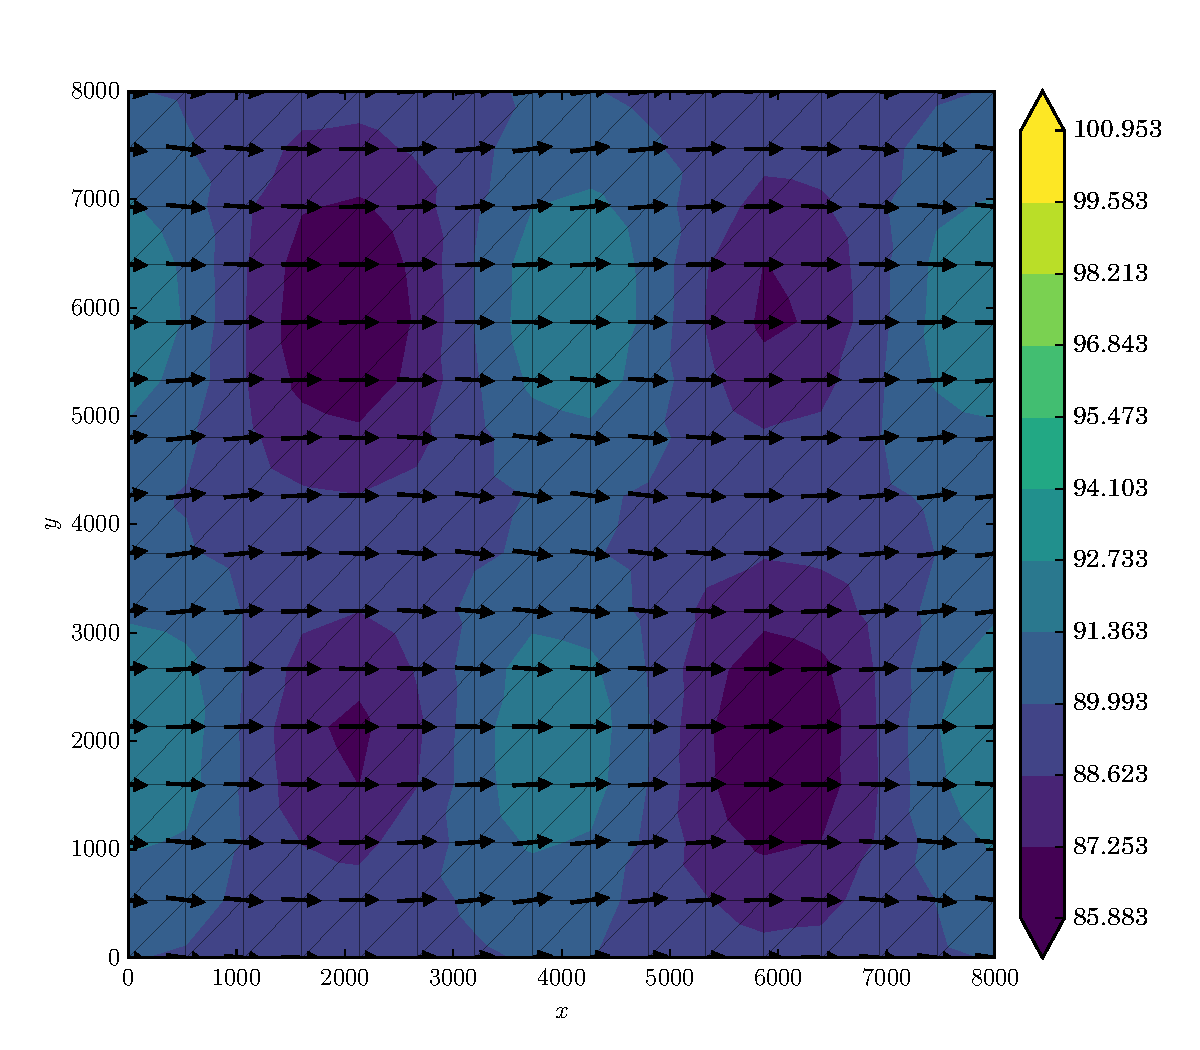
\includegraphics[width=\linewidth]{images/stress_balance/FS/U_mag.pdf}
  \caption{$\rankone{u}_S$}
  \label{fs_ms_U}
  \end{subfigure}
  \begin{subfigure}[b]{0.3\linewidth}
    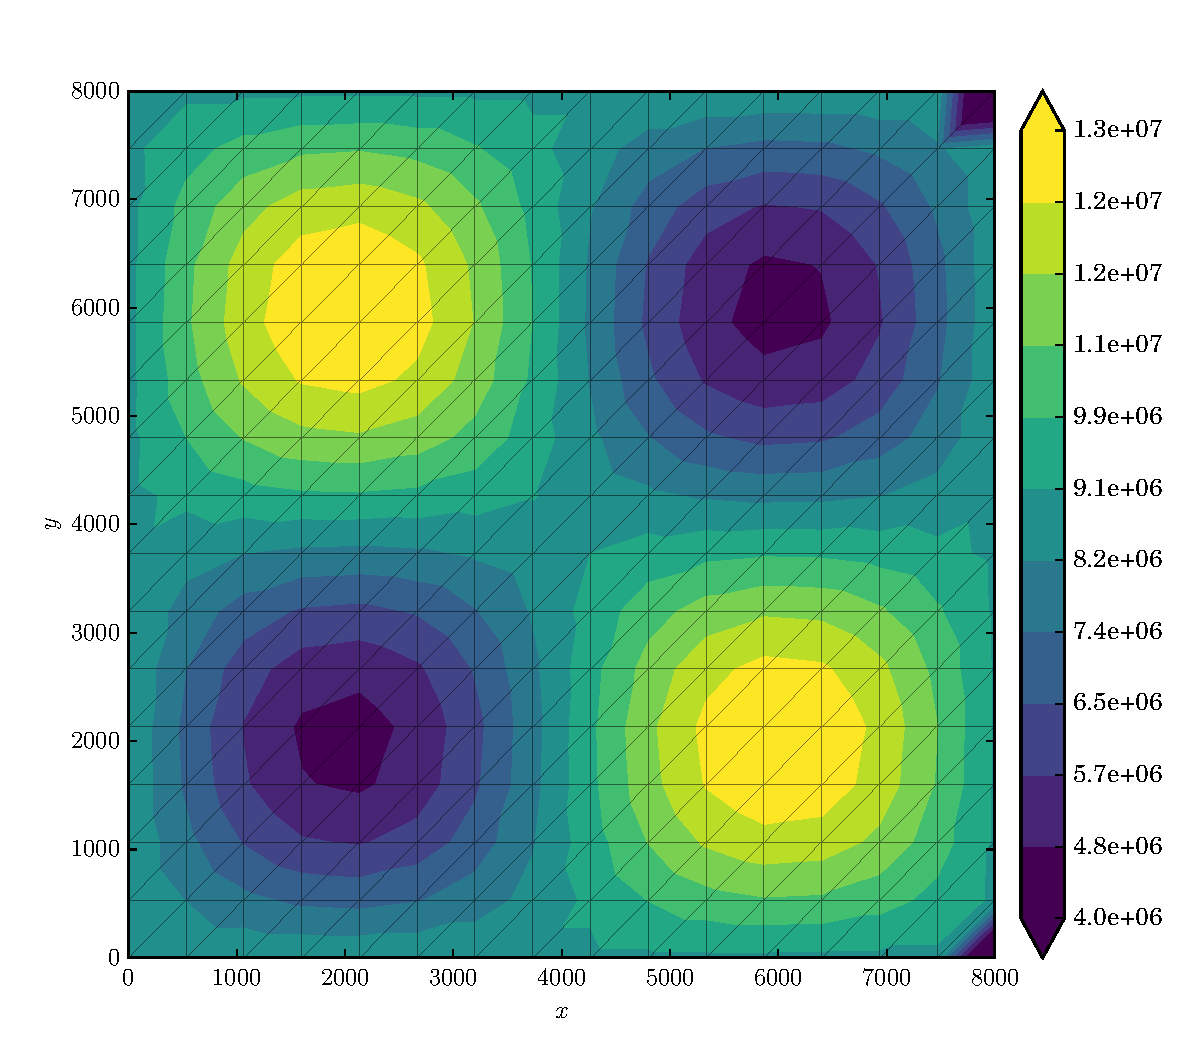
\includegraphics[width=\linewidth]{images/stress_balance/FS/p.pdf}
  \caption{$p |_B$}
  \label{fs_ms_p}
  \end{subfigure}

  \begin{subfigure}[b]{0.3\linewidth}
    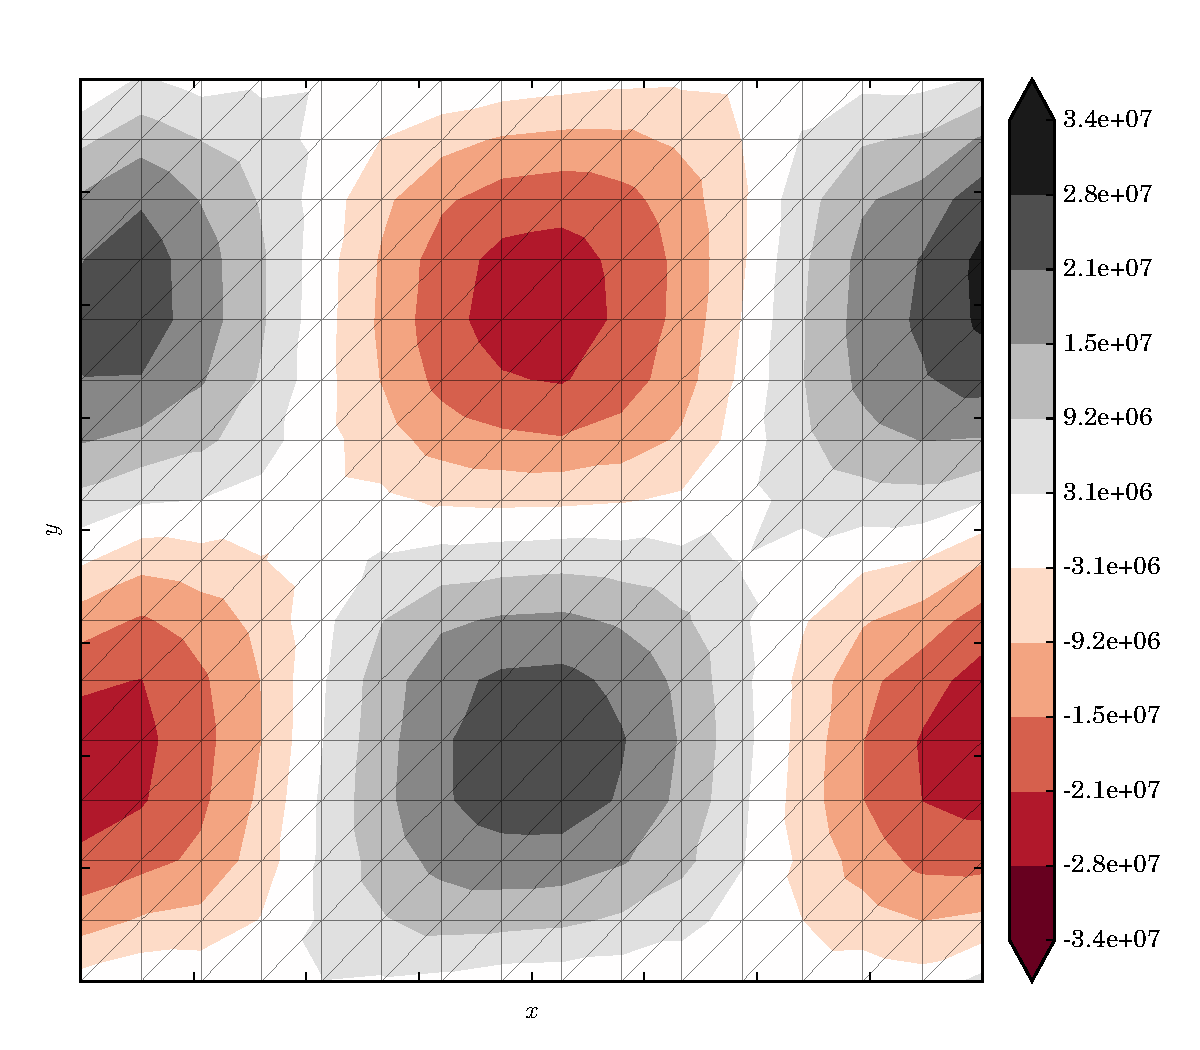
\includegraphics[width=\linewidth]{images/stress_balance/FS/N_ii.pdf}
  \caption{$N_{ii}$}
  \label{fs_N_ii}
  \end{subfigure}
  \begin{subfigure}[b]{0.3\linewidth}
    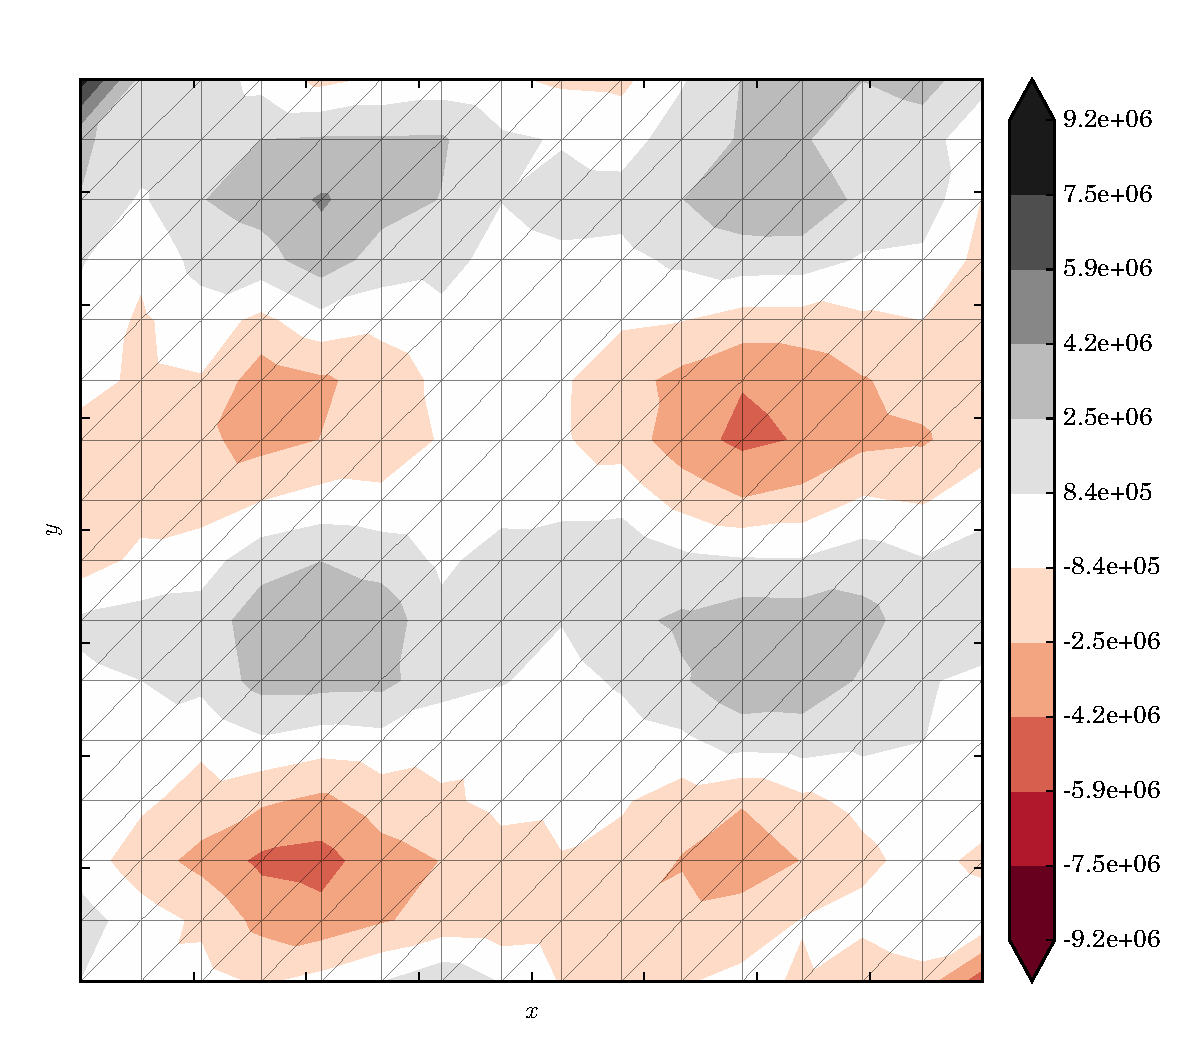
\includegraphics[width=\linewidth]{images/stress_balance/FS/N_ij.pdf}
  \caption{$N_{ij}$}
  \label{fs_N_ij}
  \end{subfigure}
  \begin{subfigure}[b]{0.3\linewidth}
    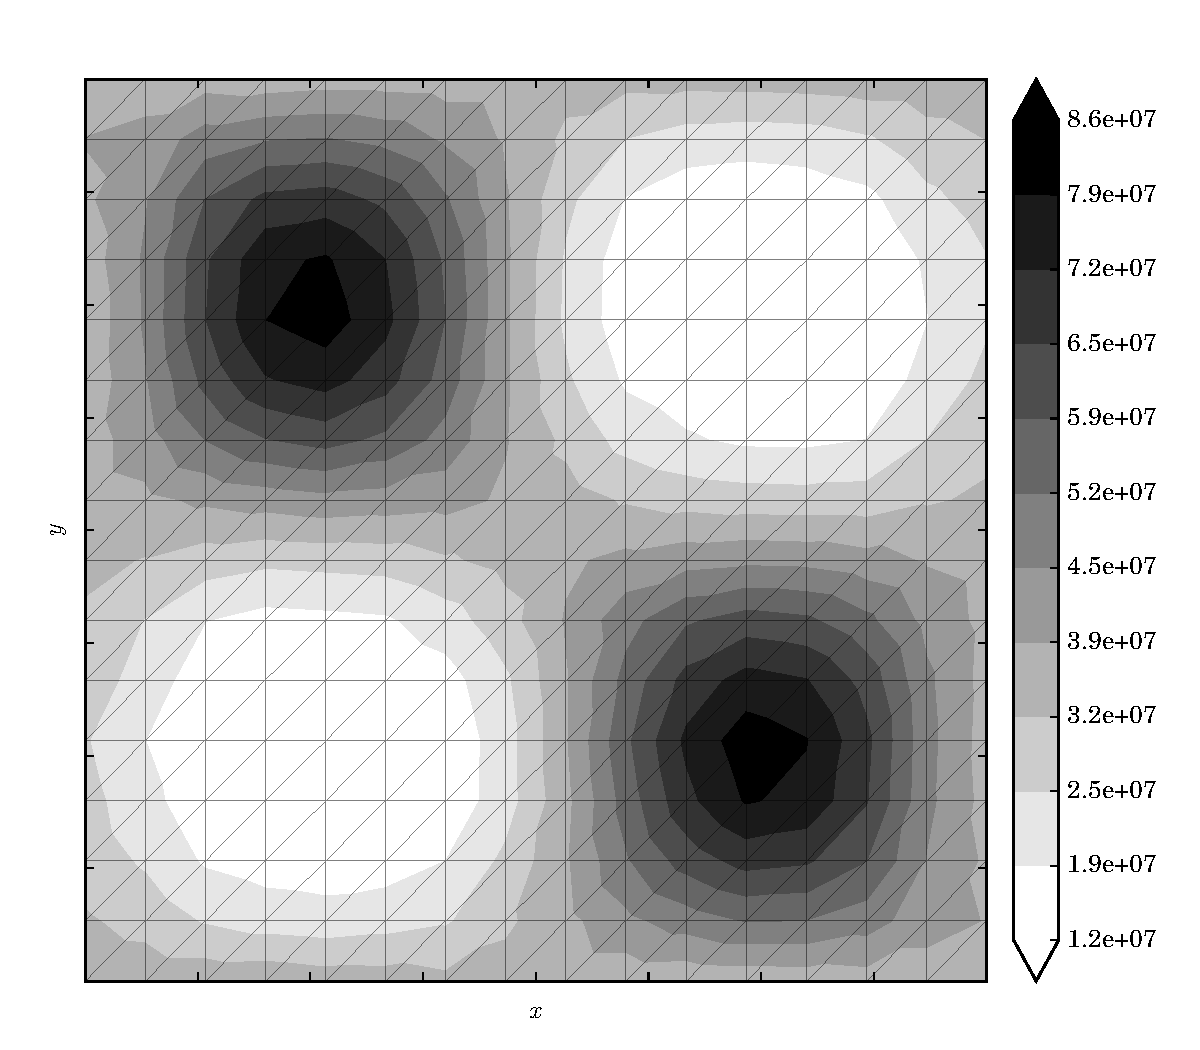
\includegraphics[width=\linewidth]{images/stress_balance/FS/N_iz.pdf}
  \caption{$N_{iz}$}
  \label{fs_N_iz}
  \end{subfigure}

  \begin{subfigure}[b]{0.3\linewidth}
    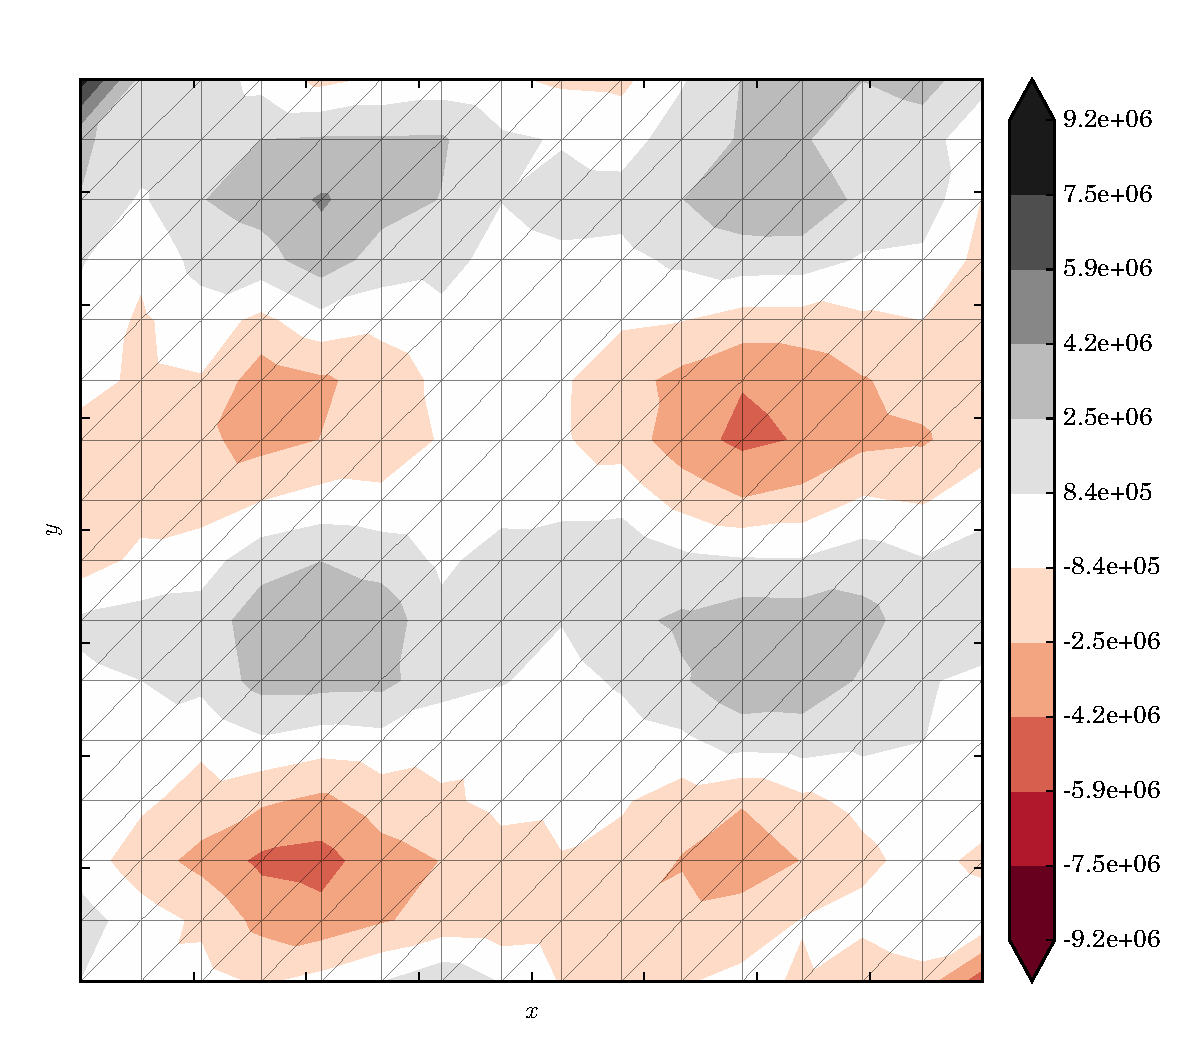
\includegraphics[width=\linewidth]{images/stress_balance/FS/N_ji.pdf}
  \caption{$N_{ji}$}
  \label{fs_N_ji}
  \end{subfigure}
  \begin{subfigure}[b]{0.3\linewidth}
    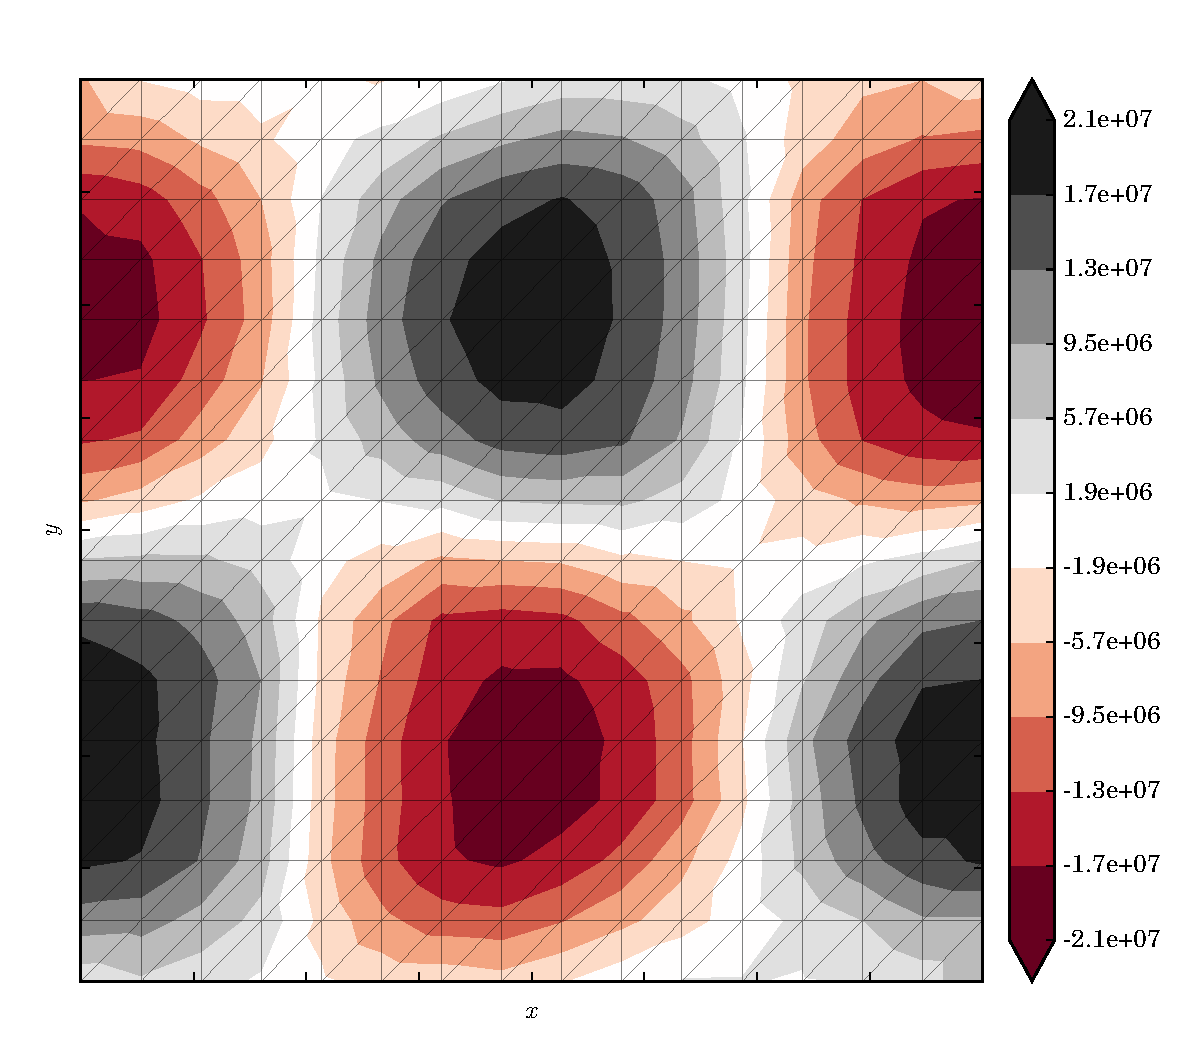
\includegraphics[width=\linewidth]{images/stress_balance/FS/N_jj.pdf}
  \caption{$N_{jj}$}
  \label{fs_N_jj}
  \end{subfigure}
  \begin{subfigure}[b]{0.3\linewidth}
    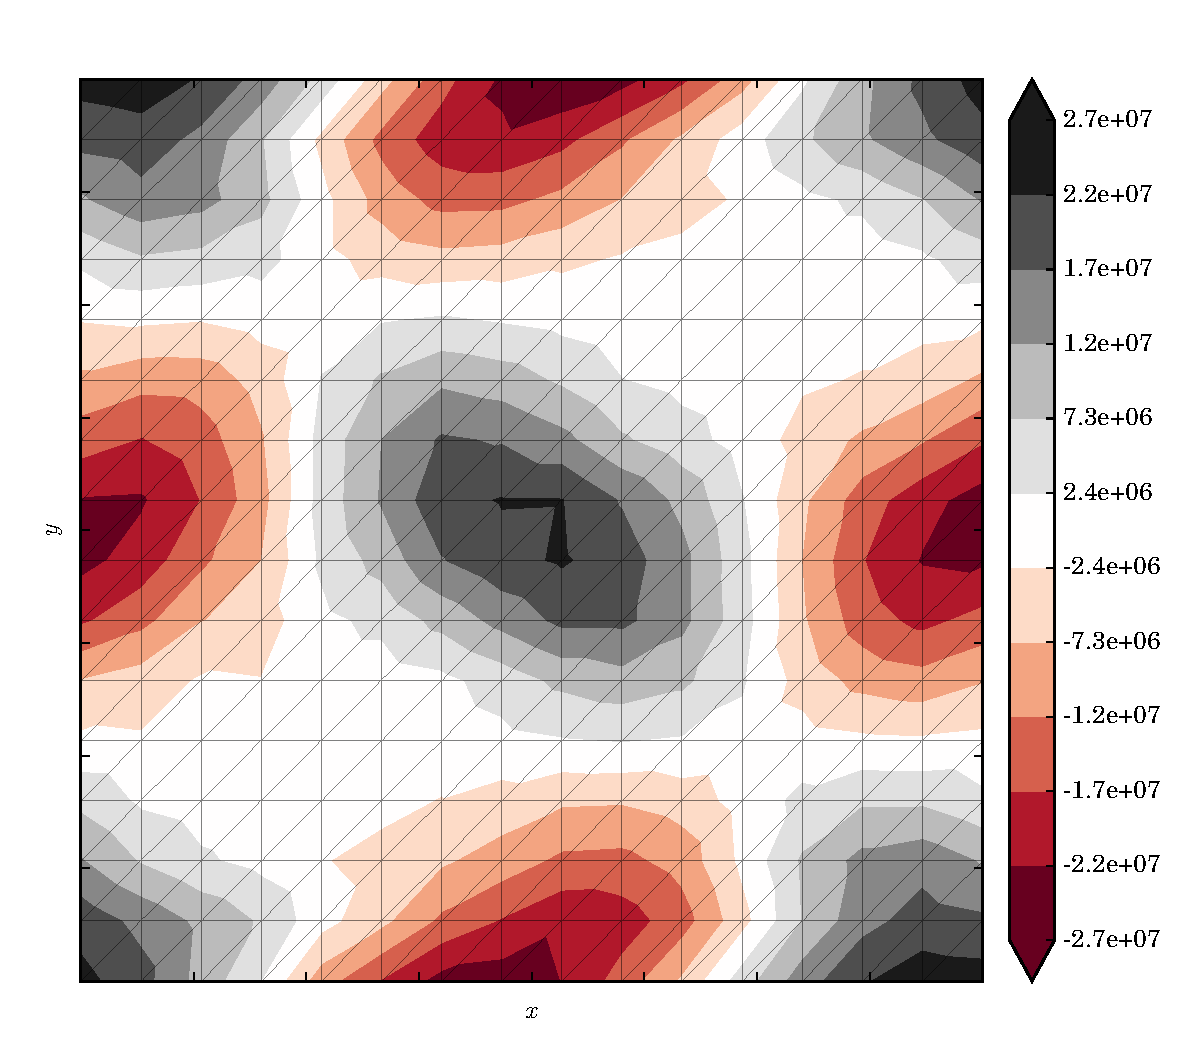
\includegraphics[width=\linewidth]{images/stress_balance/FS/N_jz.pdf}
  \caption{$N_{jz}$}
  \label{fs_N_jz}
  \end{subfigure}

  \begin{subfigure}[b]{0.3\linewidth}
    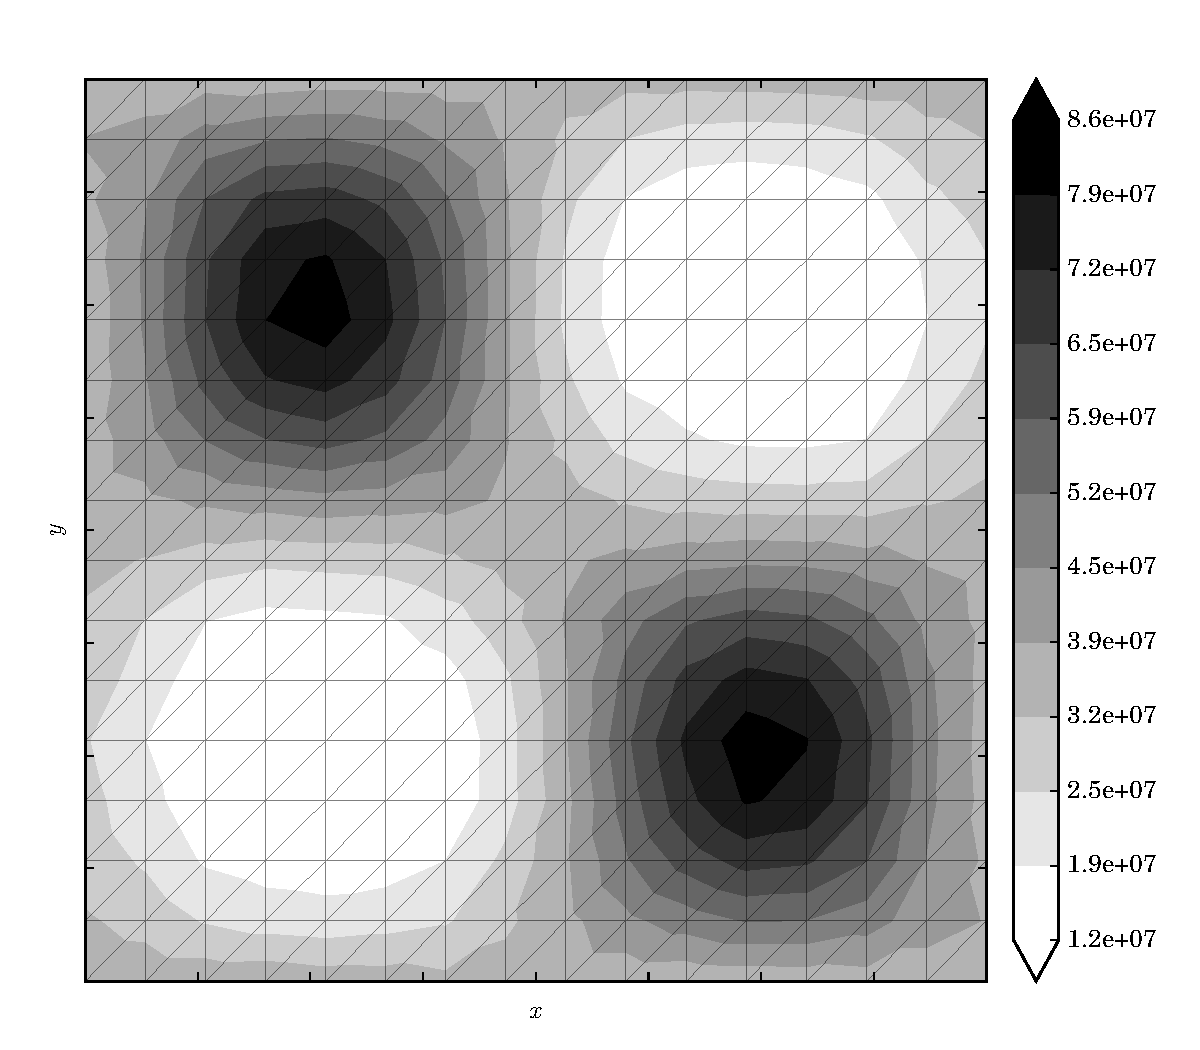
\includegraphics[width=\linewidth]{images/stress_balance/FS/N_zi.pdf}
  \caption{$N_{zi}$}
  \label{fs_N_zi}
  \end{subfigure}
  \begin{subfigure}[b]{0.3\linewidth}
    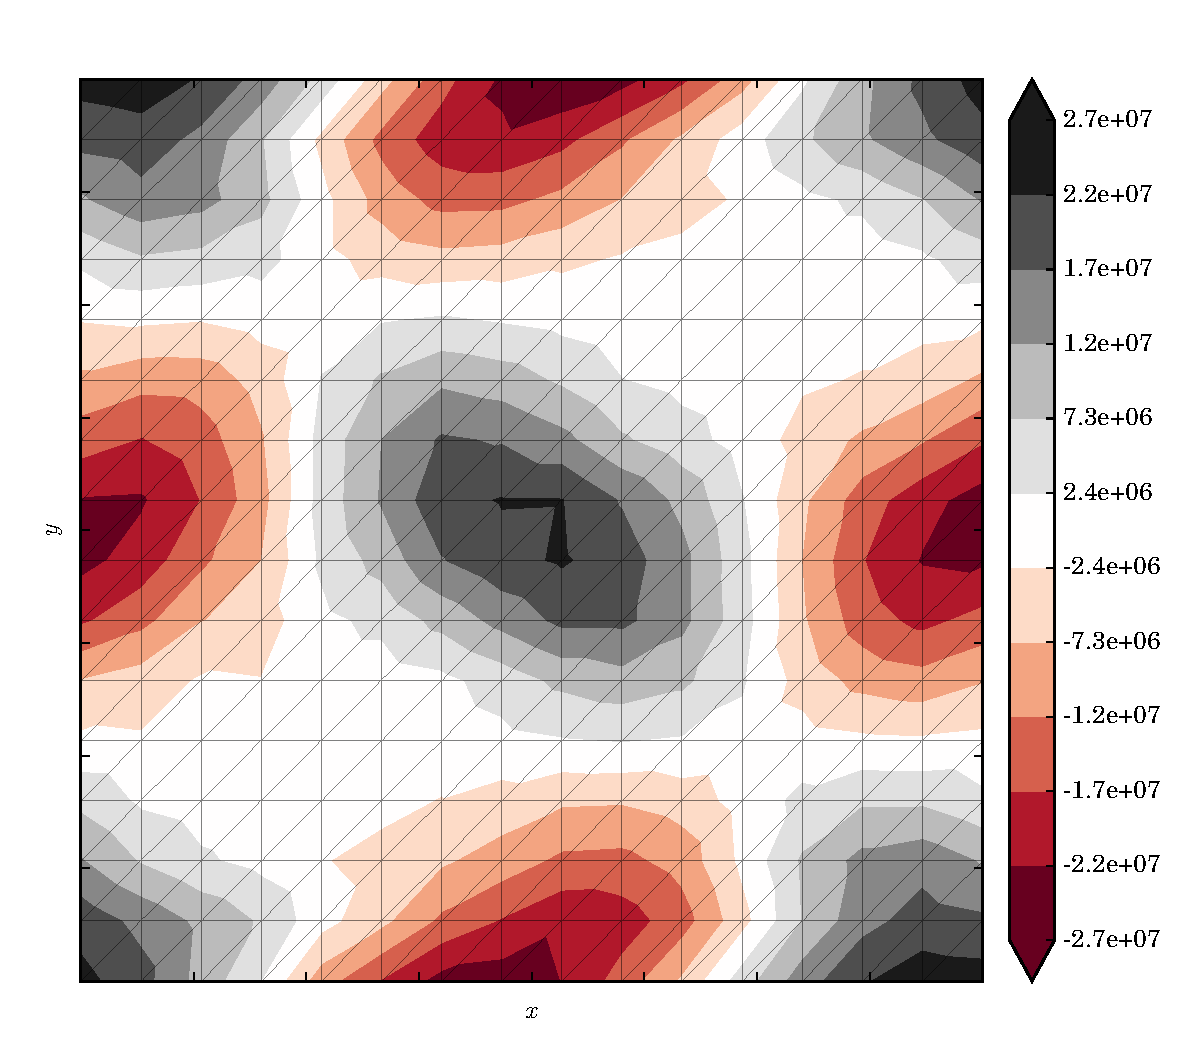
\includegraphics[width=\linewidth]{images/stress_balance/FS/N_zj.pdf}
  \caption{$N_{zj}$}
  \label{fs_N_zj}
  \end{subfigure}
  \begin{subfigure}[b]{0.3\linewidth}
    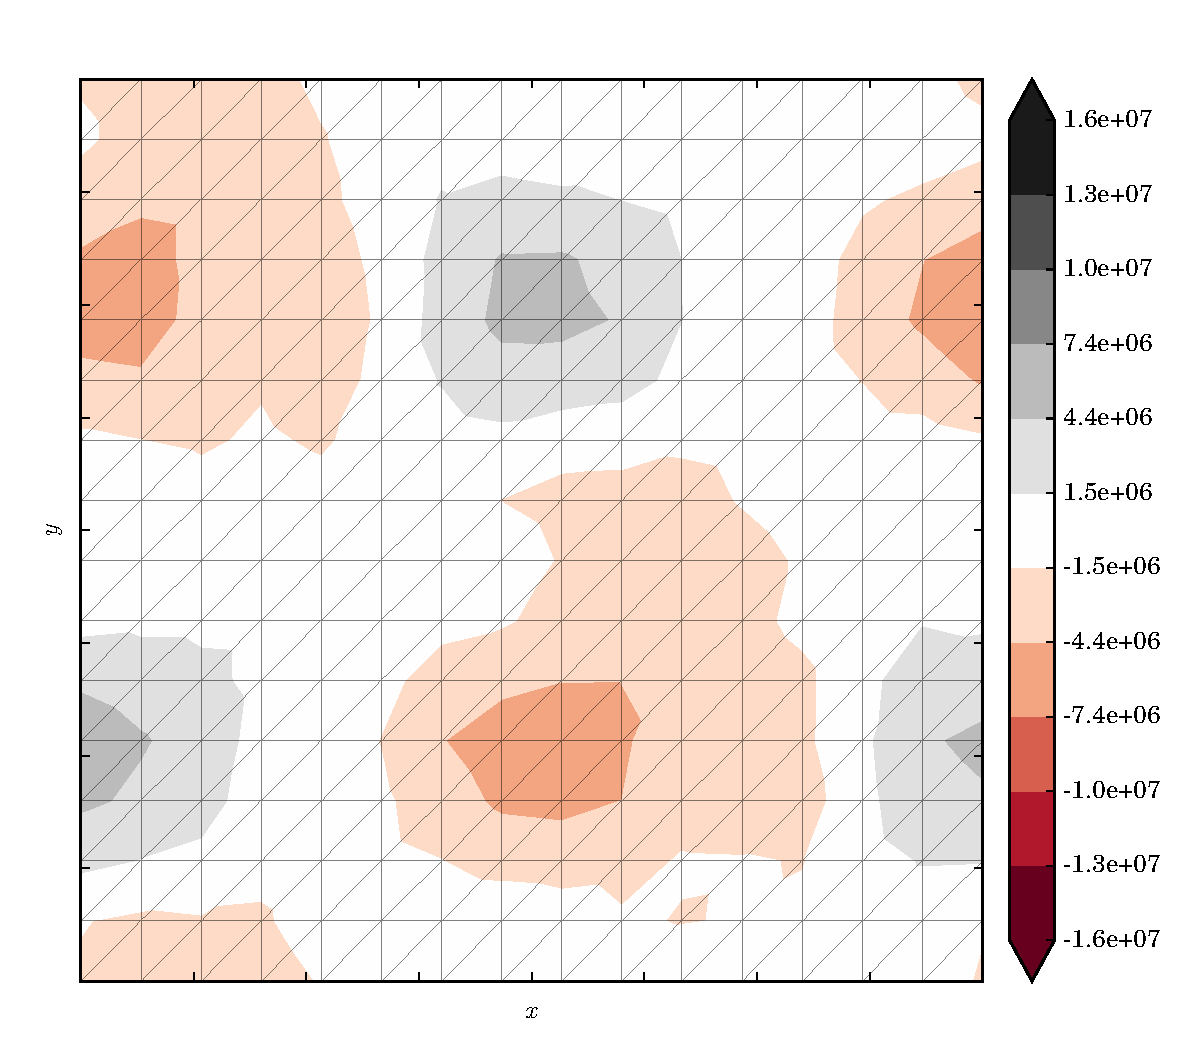
\includegraphics[width=\linewidth]{images/stress_balance/FS/N_zz.pdf}
  \caption{$N_{zz}$}
  \label{fs_N_zz}
  \end{subfigure}
 
  \caption[ISMIP-HOM full-Stokes membrane stress]{Full-Stokes membrane stress $N_{kk}$.}

  \label{fs_membrane_stress}

\end{figure*}

%===============================================================================

\begin{figure*}
  
  \centering 
  
  \begin{subfigure}[b]{0.3\linewidth}
    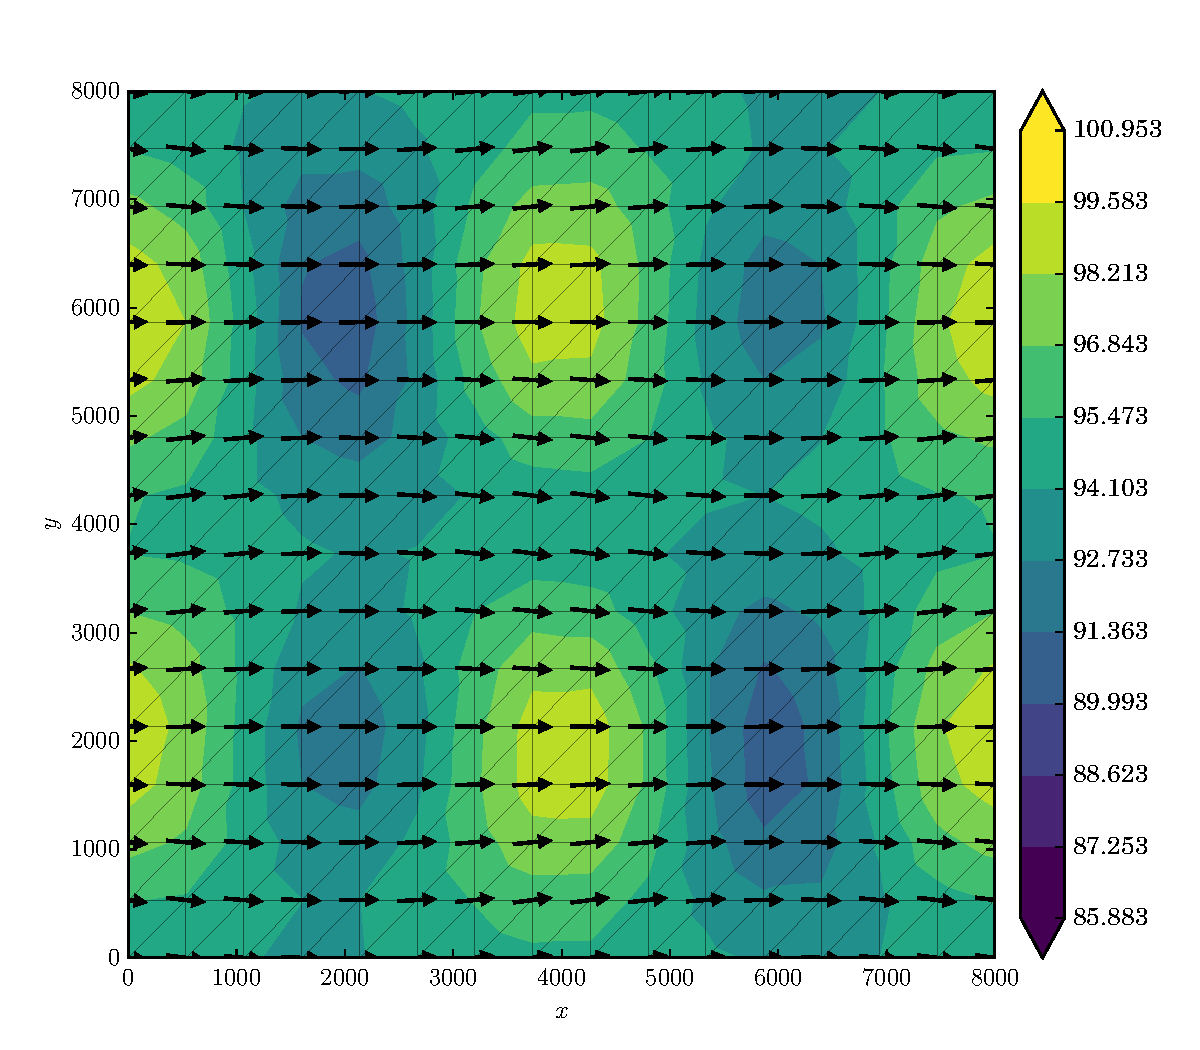
\includegraphics[width=\linewidth]{images/stress_balance/RS/U_mag.pdf}
  \caption{$\rankone{u}_S$}
  \label{rs_ms_U}
  \end{subfigure}
  \begin{subfigure}[b]{0.3\linewidth}
    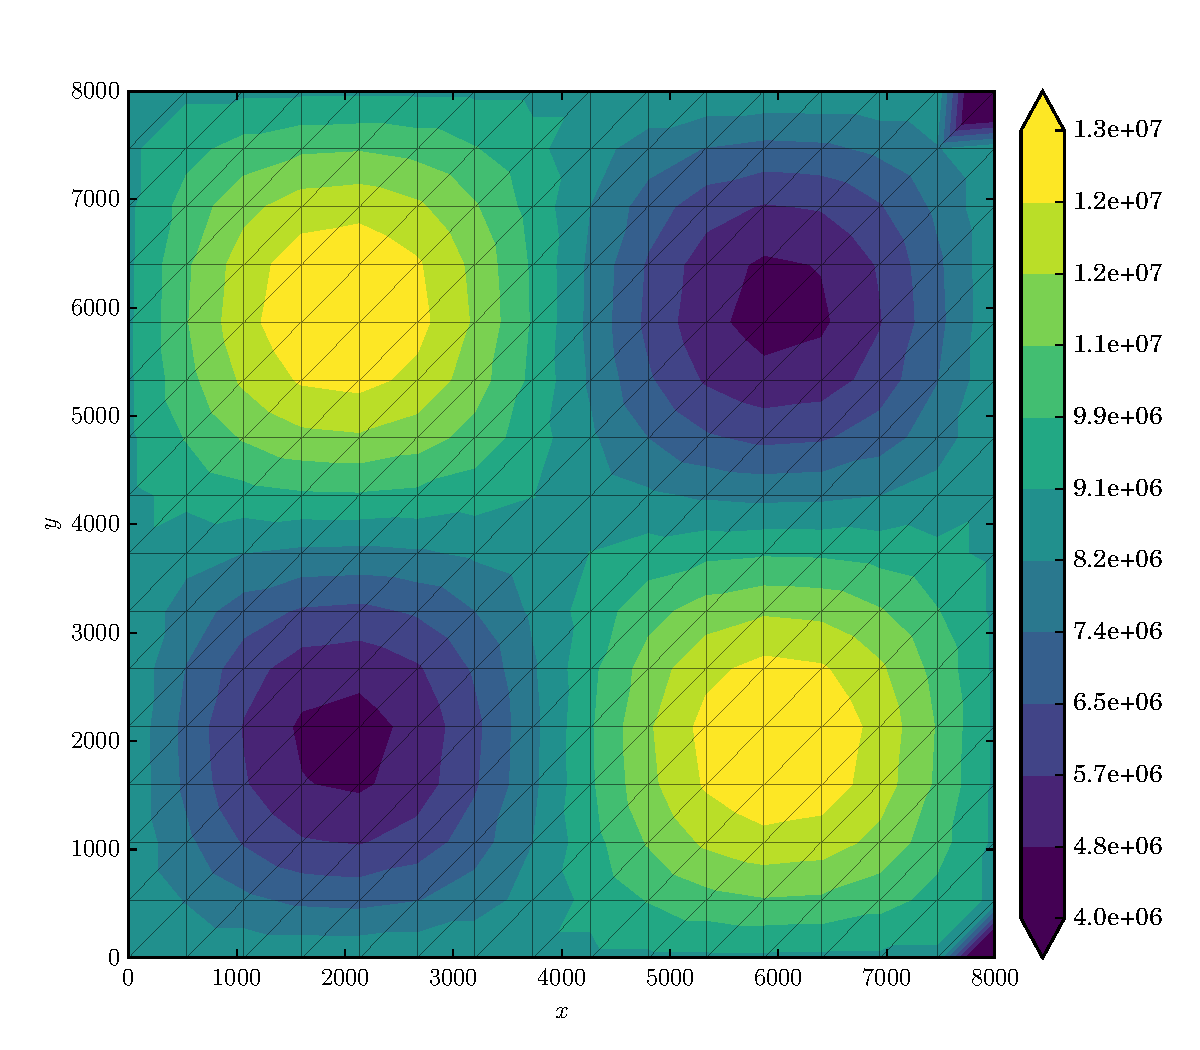
\includegraphics[width=\linewidth]{images/stress_balance/RS/p.pdf}
  \caption{$p |_B$}
  \label{rs_ms_p}
  \end{subfigure}

  \begin{subfigure}[b]{0.3\linewidth}
    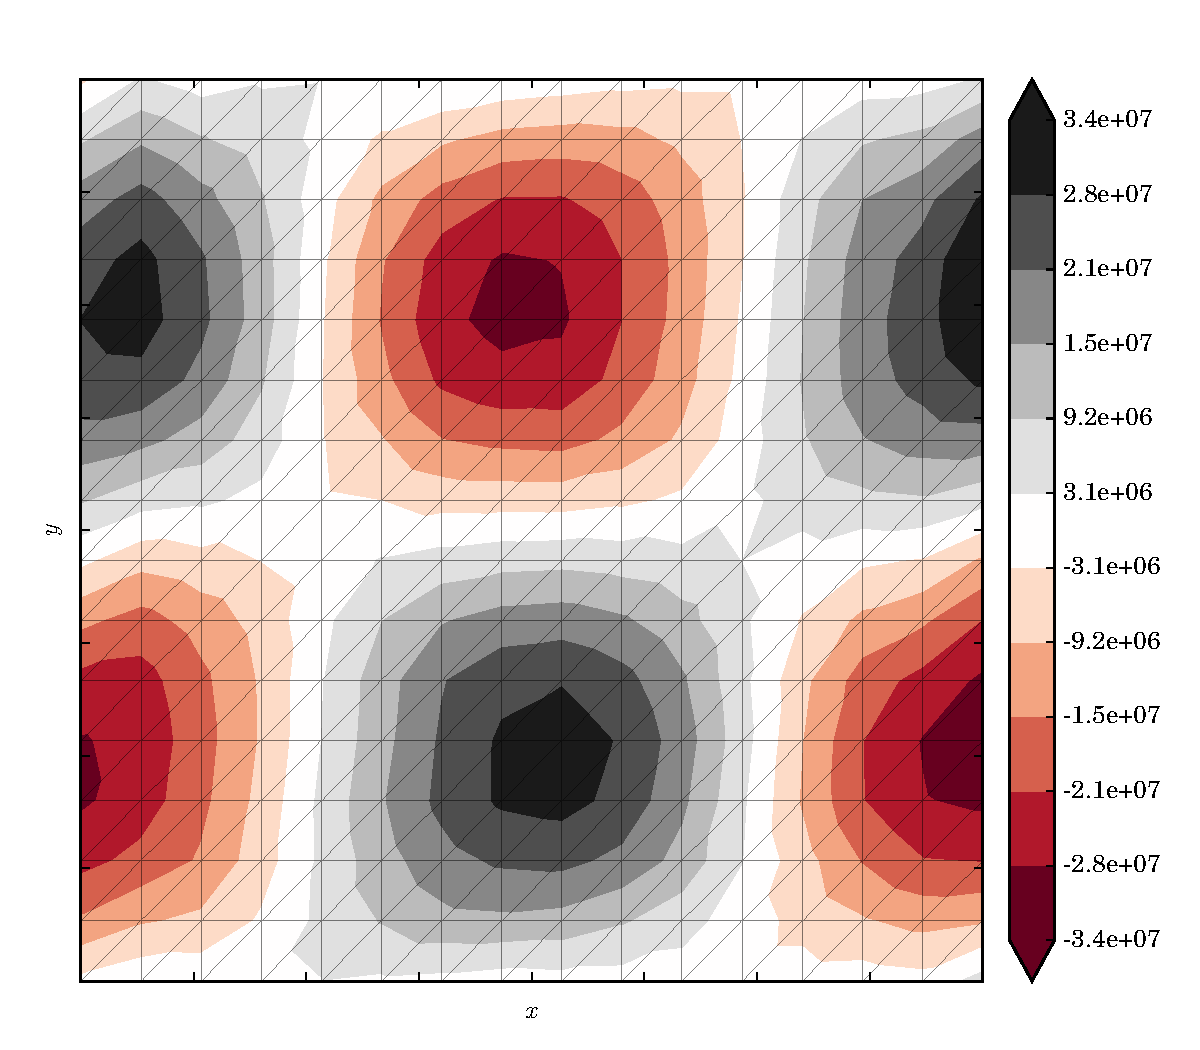
\includegraphics[width=\linewidth]{images/stress_balance/RS/N_ii.pdf}
  \caption{$N_{ii}$}
  \label{rs_N_ii}
  \end{subfigure}
  \begin{subfigure}[b]{0.3\linewidth}
    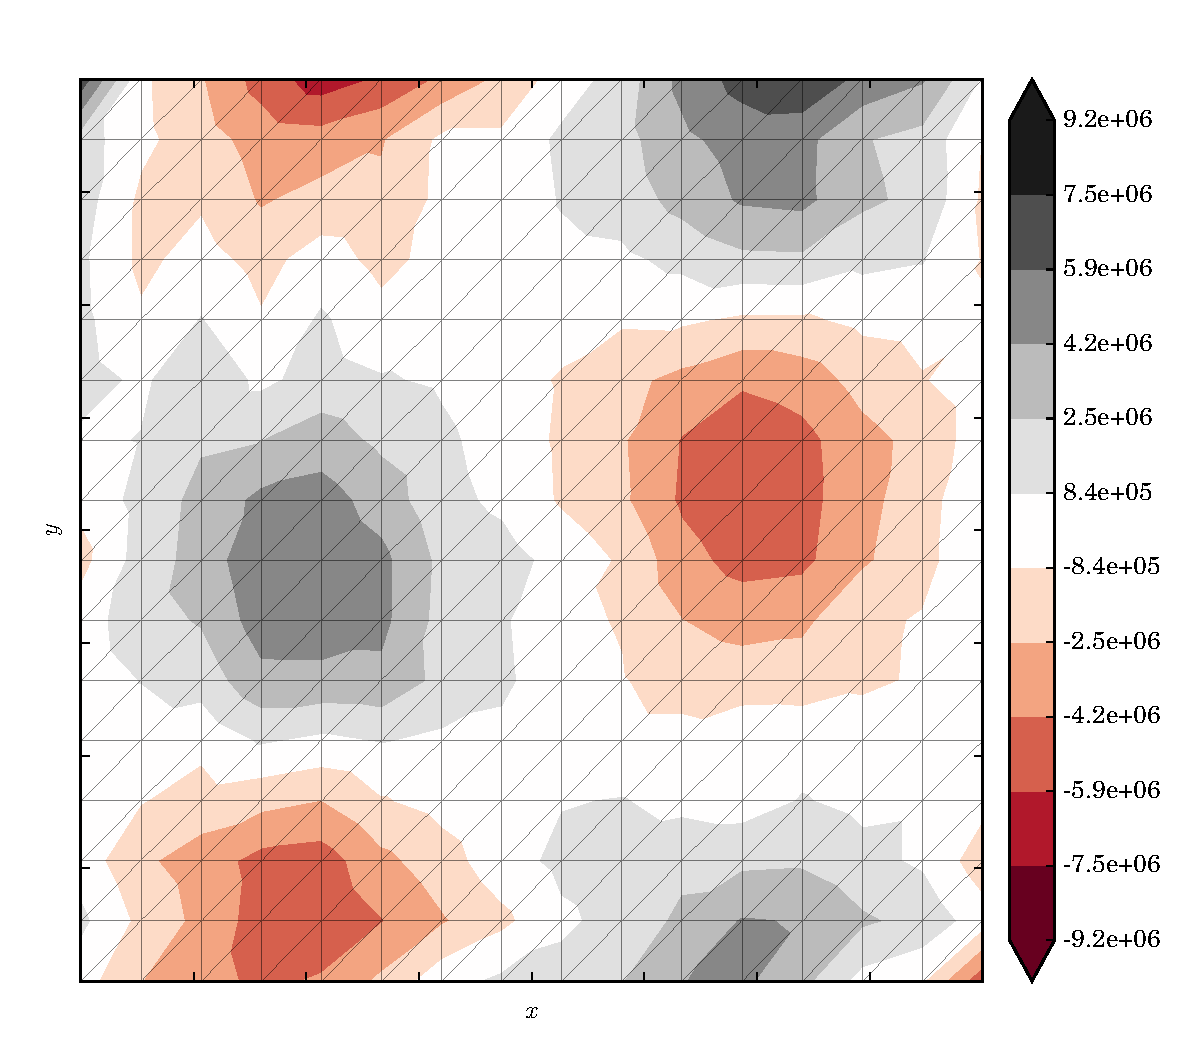
\includegraphics[width=\linewidth]{images/stress_balance/RS/N_ij.pdf}
  \caption{$N_{ij}$}
  \label{rs_N_ij}
  \end{subfigure}
  \begin{subfigure}[b]{0.3\linewidth}
    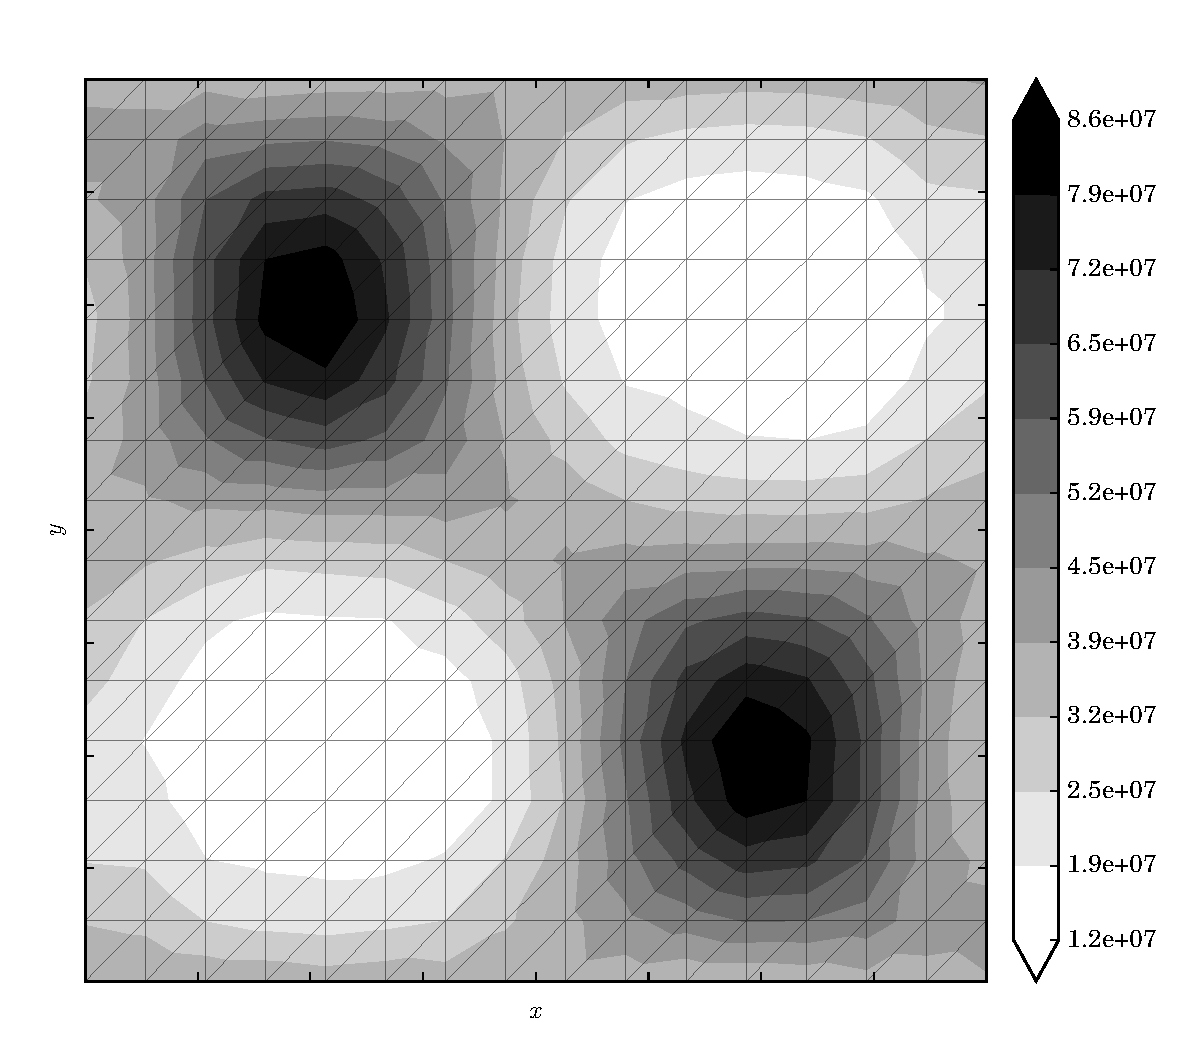
\includegraphics[width=\linewidth]{images/stress_balance/RS/N_iz.pdf}
  \caption{$N_{iz}$}
  \label{rs_N_iz}
  \end{subfigure}

  \begin{subfigure}[b]{0.3\linewidth}
    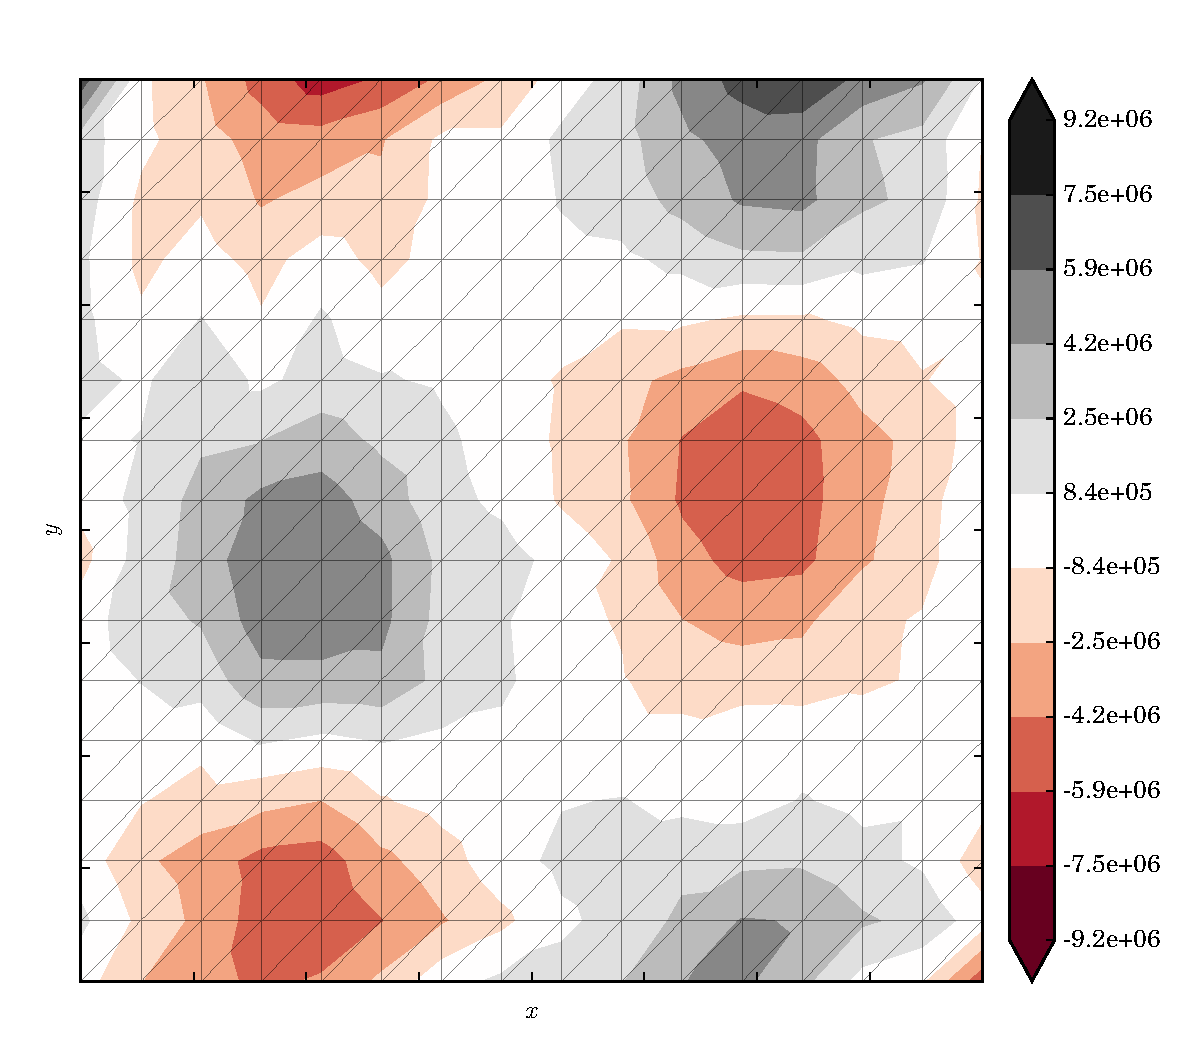
\includegraphics[width=\linewidth]{images/stress_balance/RS/N_ji.pdf}
  \caption{$N_{ji}$}
  \label{rs_N_ji}
  \end{subfigure}
  \begin{subfigure}[b]{0.3\linewidth}
    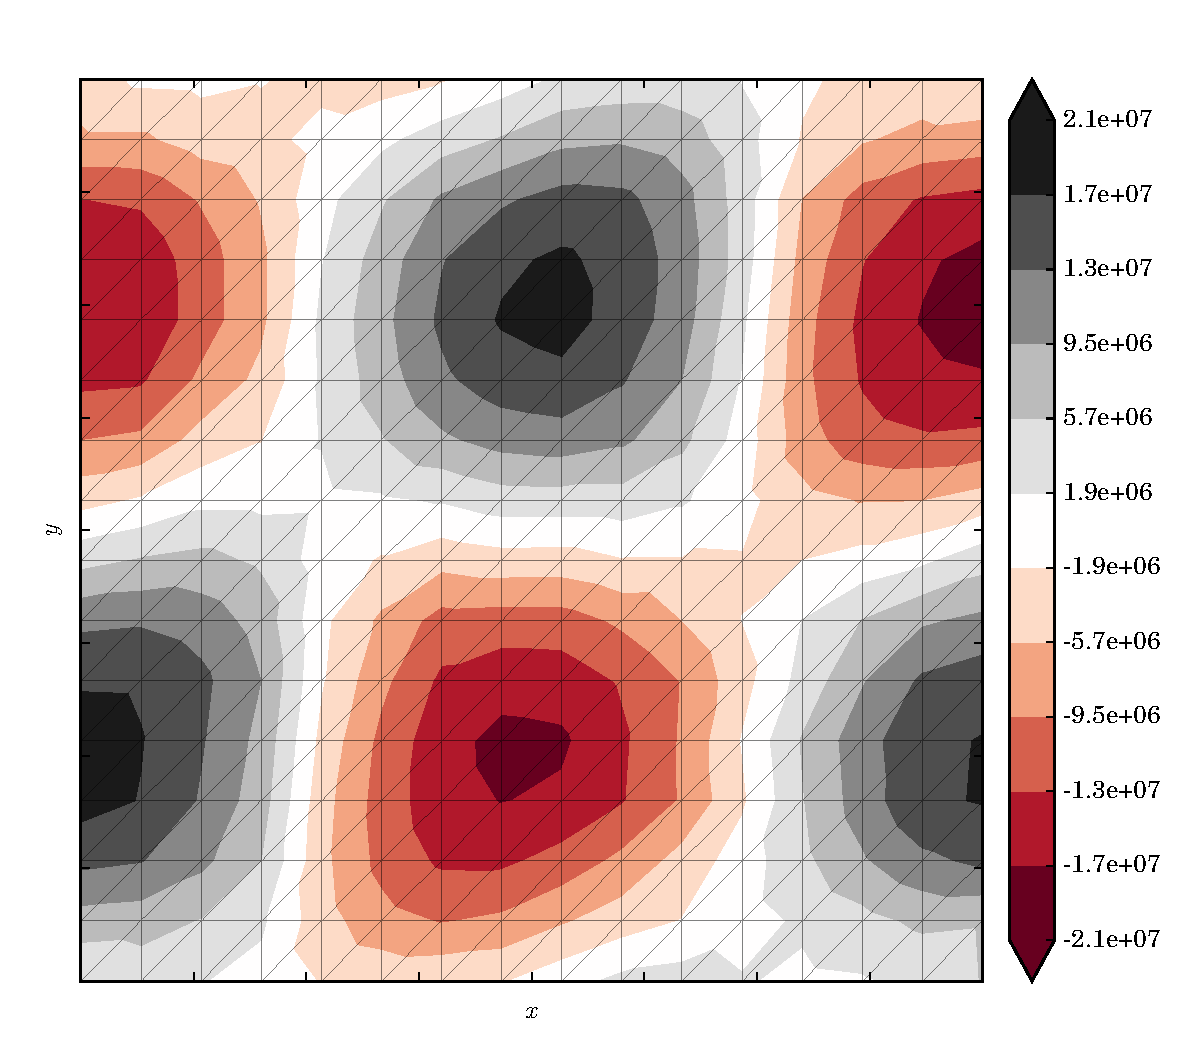
\includegraphics[width=\linewidth]{images/stress_balance/RS/N_jj.pdf}
  \caption{$N_{jj}$}
  \label{rs_N_jj}
  \end{subfigure}
  \begin{subfigure}[b]{0.3\linewidth}
    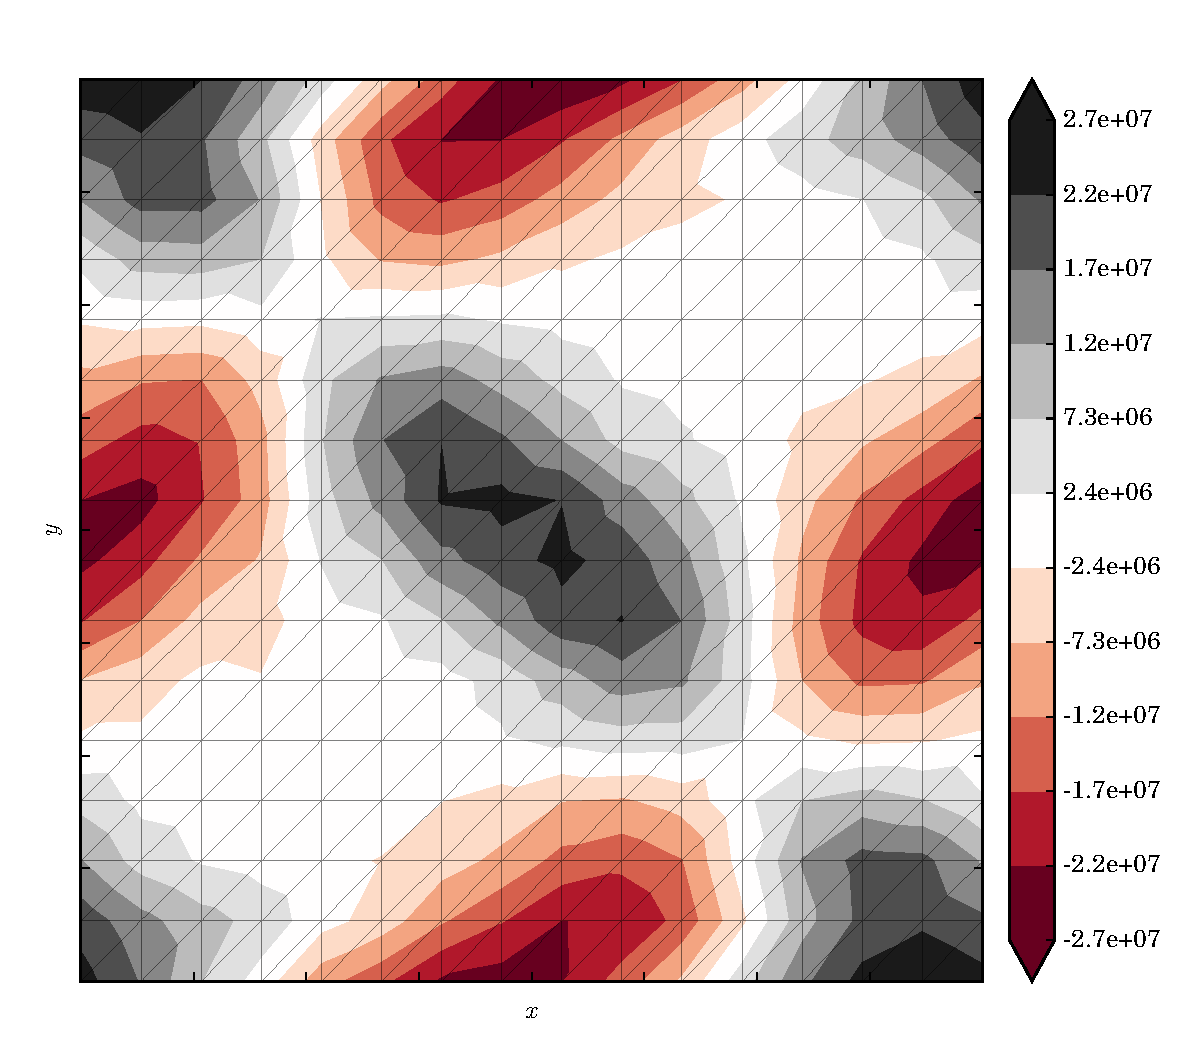
\includegraphics[width=\linewidth]{images/stress_balance/RS/N_jz.pdf}
  \caption{$N_{jz}$}
  \label{rs_N_jz}
  \end{subfigure}

  \begin{subfigure}[b]{0.3\linewidth}
    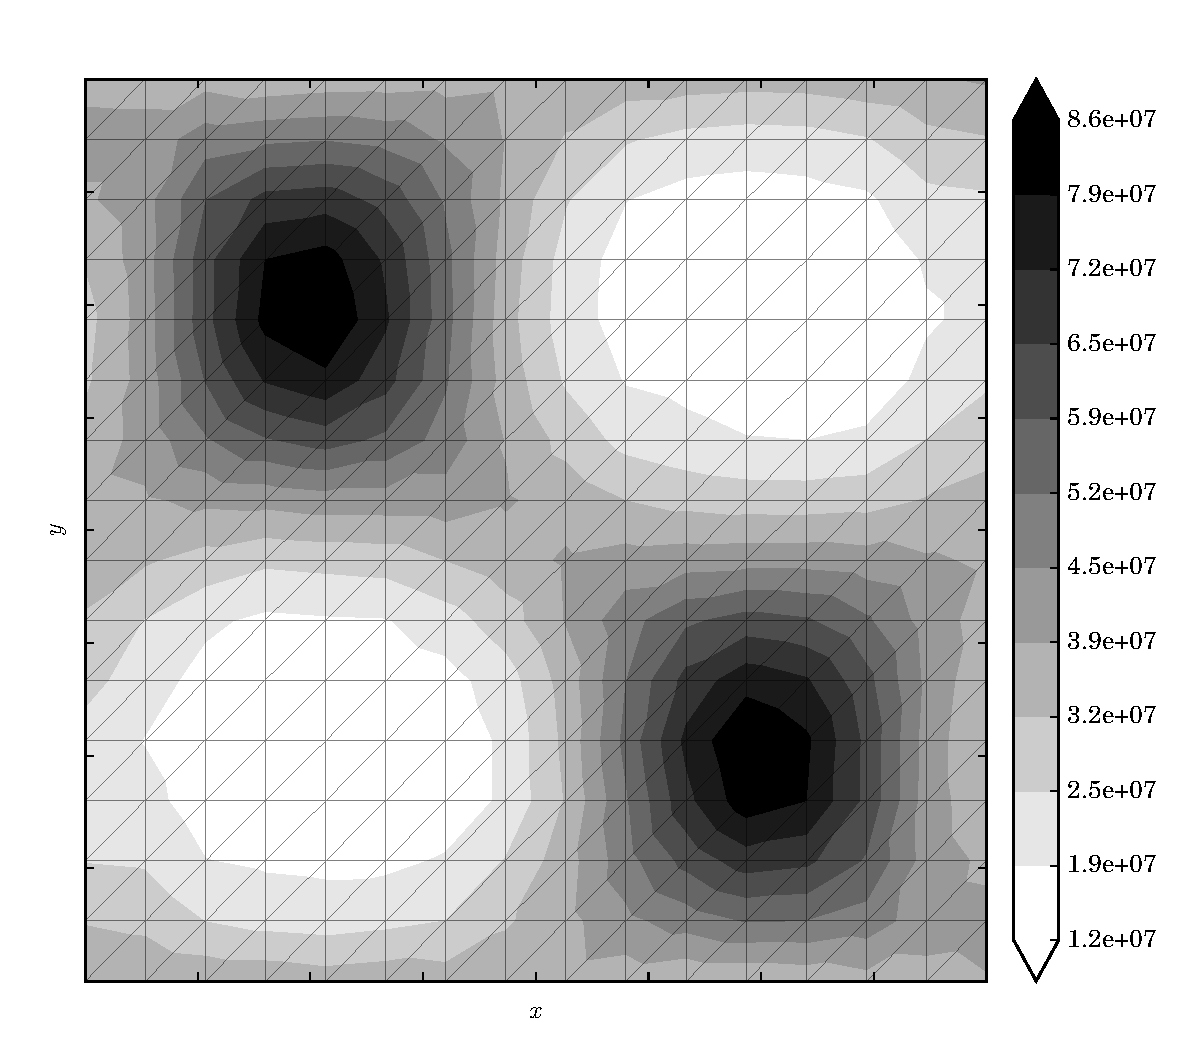
\includegraphics[width=\linewidth]{images/stress_balance/RS/N_zi.pdf}
  \caption{$N_{zi}$}
  \label{rs_N_zi}
  \end{subfigure}
  \begin{subfigure}[b]{0.3\linewidth}
    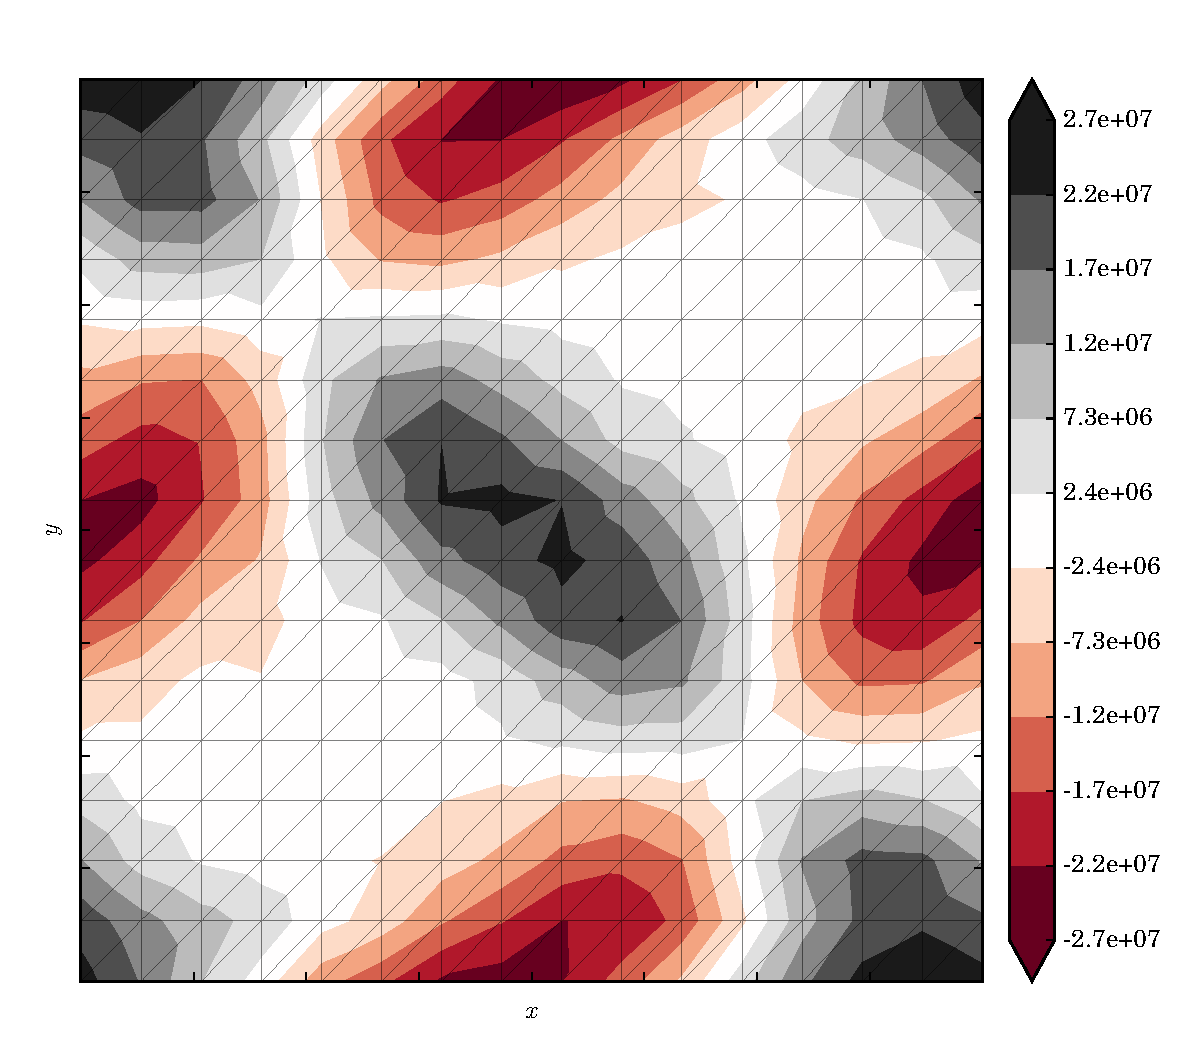
\includegraphics[width=\linewidth]{images/stress_balance/RS/N_zj.pdf}
  \caption{$N_{zj}$}
  \label{rs_N_zj}
  \end{subfigure}
  \begin{subfigure}[b]{0.3\linewidth}
    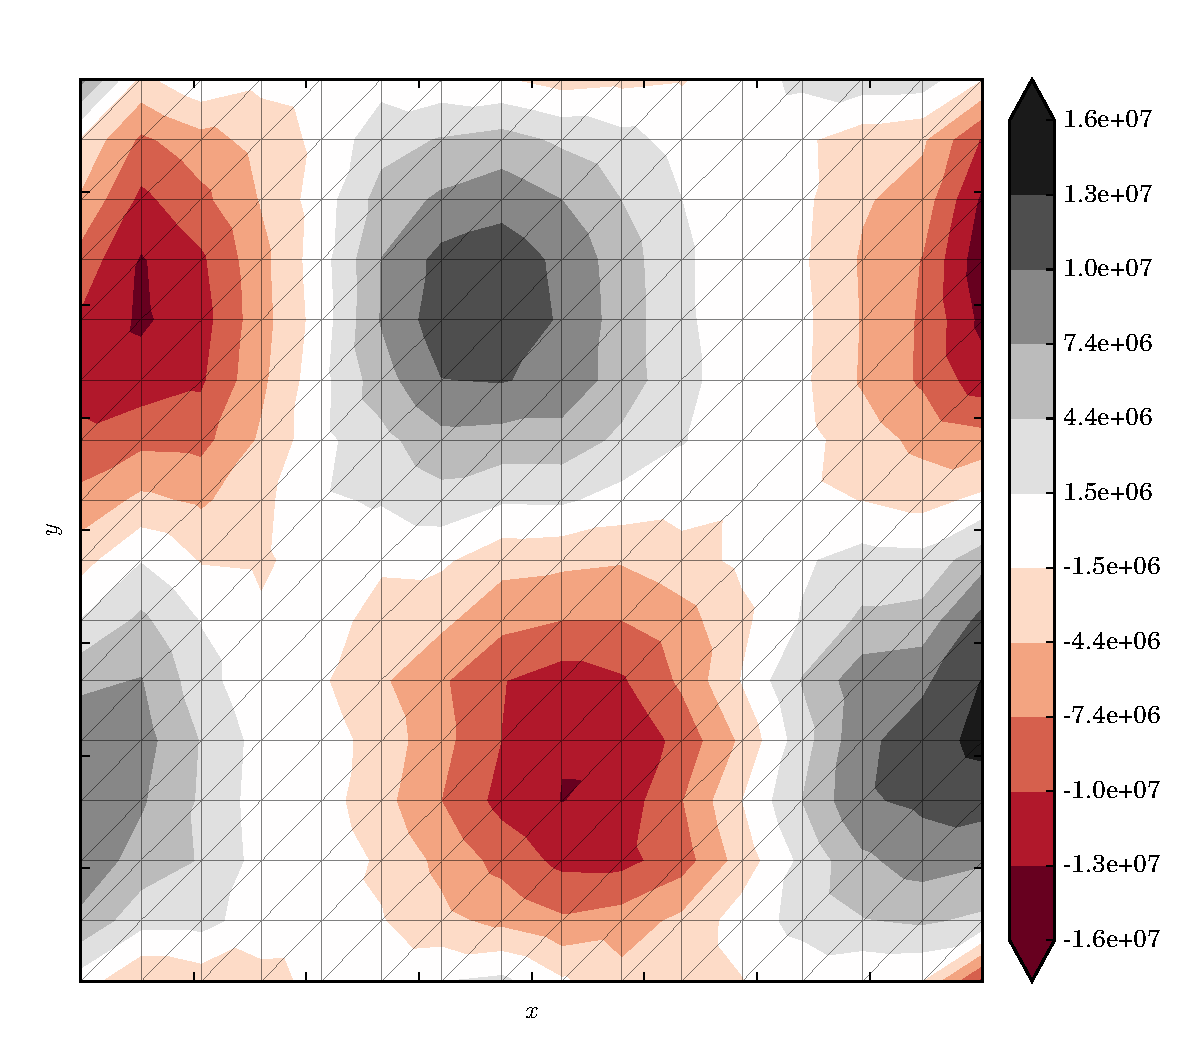
\includegraphics[width=\linewidth]{images/stress_balance/RS/N_zz.pdf}
  \caption{$N_{zz}$}
  \label{rs_N_zz}
  \end{subfigure}
 
  \caption[ISMIP-HOM reformulated-Stokes membrane stress]{Reformulated-Stokes membrane stress $N_{kk}$.}

  \label{rs_membrane_stress}

\end{figure*}

%===============================================================================

\begin{figure*}
  
  \centering 

  \begin{subfigure}[b]{0.3\linewidth}
    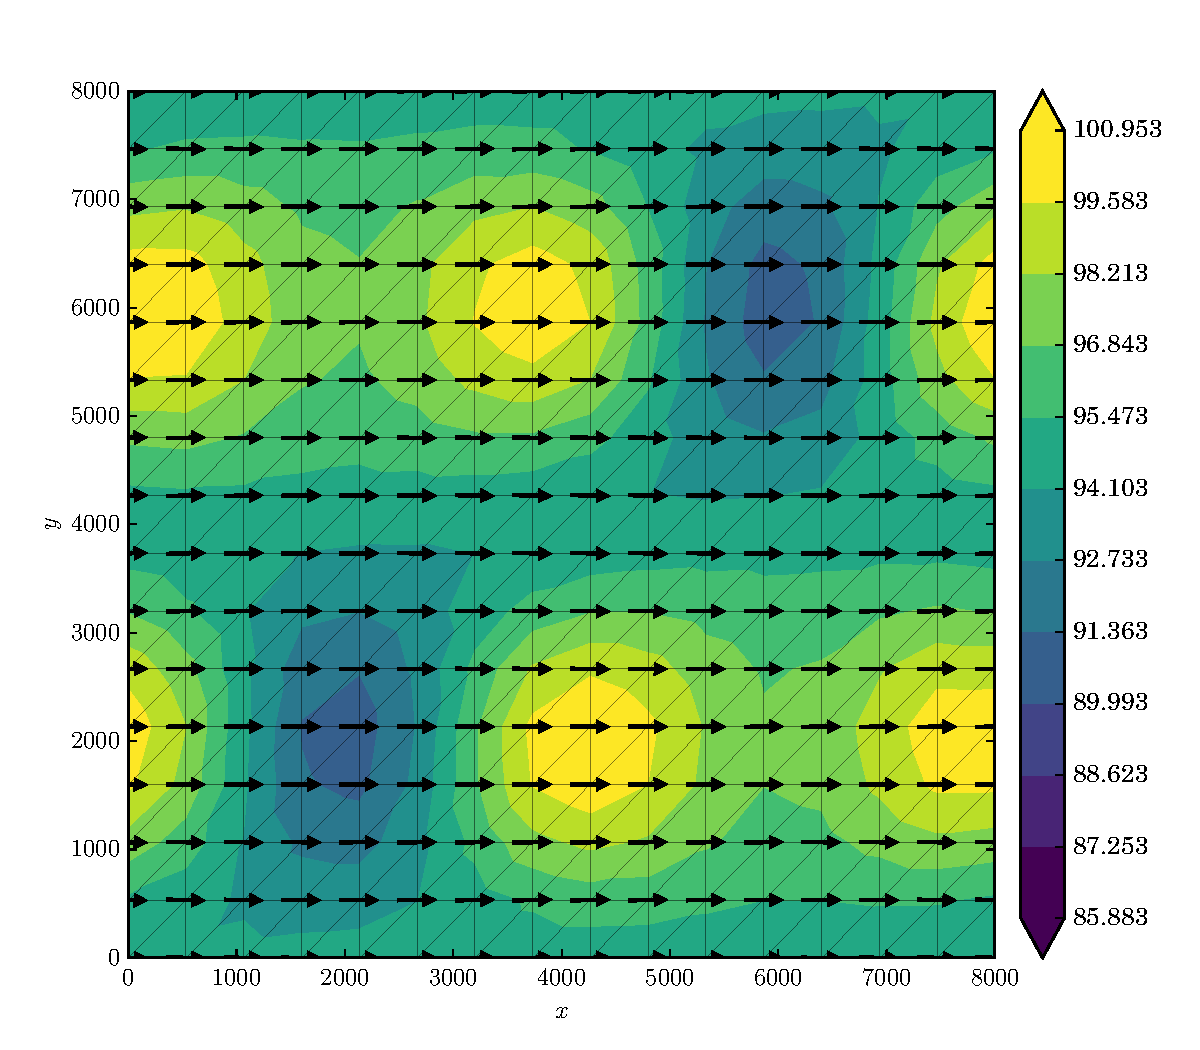
\includegraphics[width=\linewidth]{images/stress_balance/BP/U_mag.pdf}
  \caption{$\rankone{u}_S$}
  \label{bp_ms_U}
  \end{subfigure}
  \begin{subfigure}[b]{0.3\linewidth}
    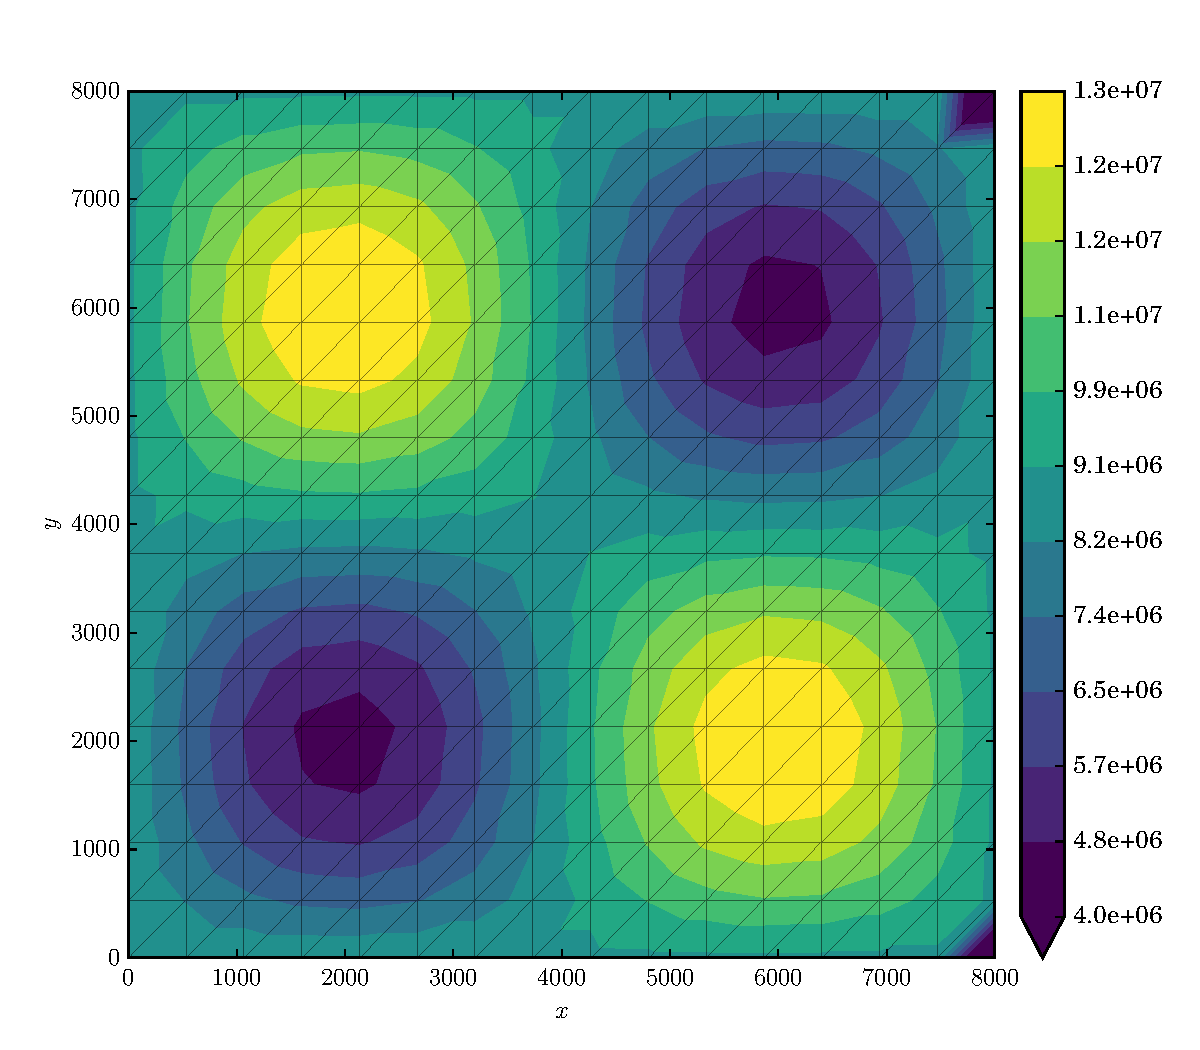
\includegraphics[width=\linewidth]{images/stress_balance/BP/p.pdf}
  \caption{$p |_B$}
  \label{bp_ms_p}
  \end{subfigure}

  \begin{subfigure}[b]{0.3\linewidth}
    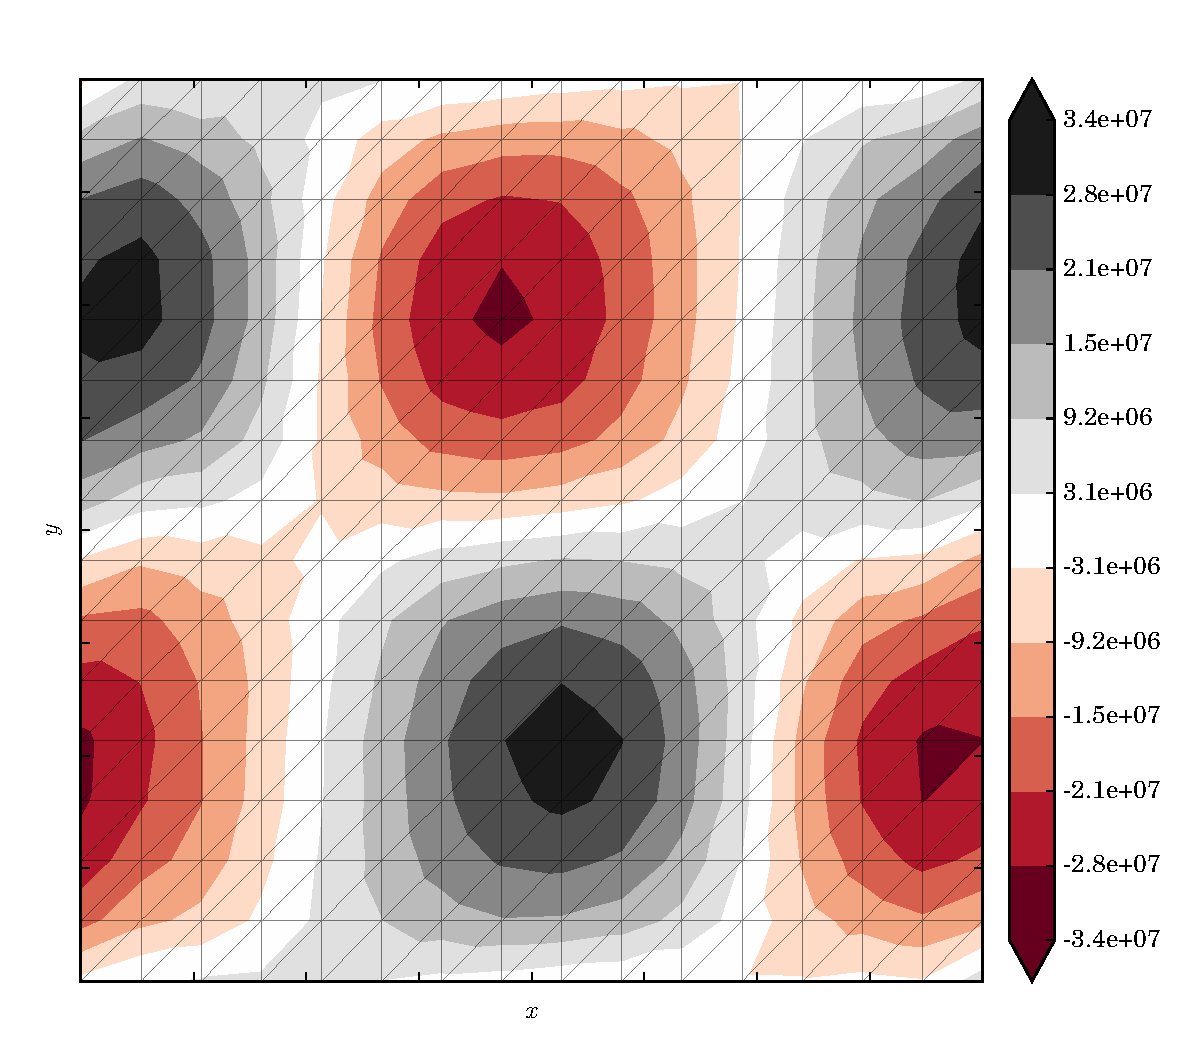
\includegraphics[width=\linewidth]{images/stress_balance/BP/N_ii.pdf}
  \caption{$N_{ii}$}
  \label{bp_N_ii}
  \end{subfigure}
  \begin{subfigure}[b]{0.3\linewidth}
    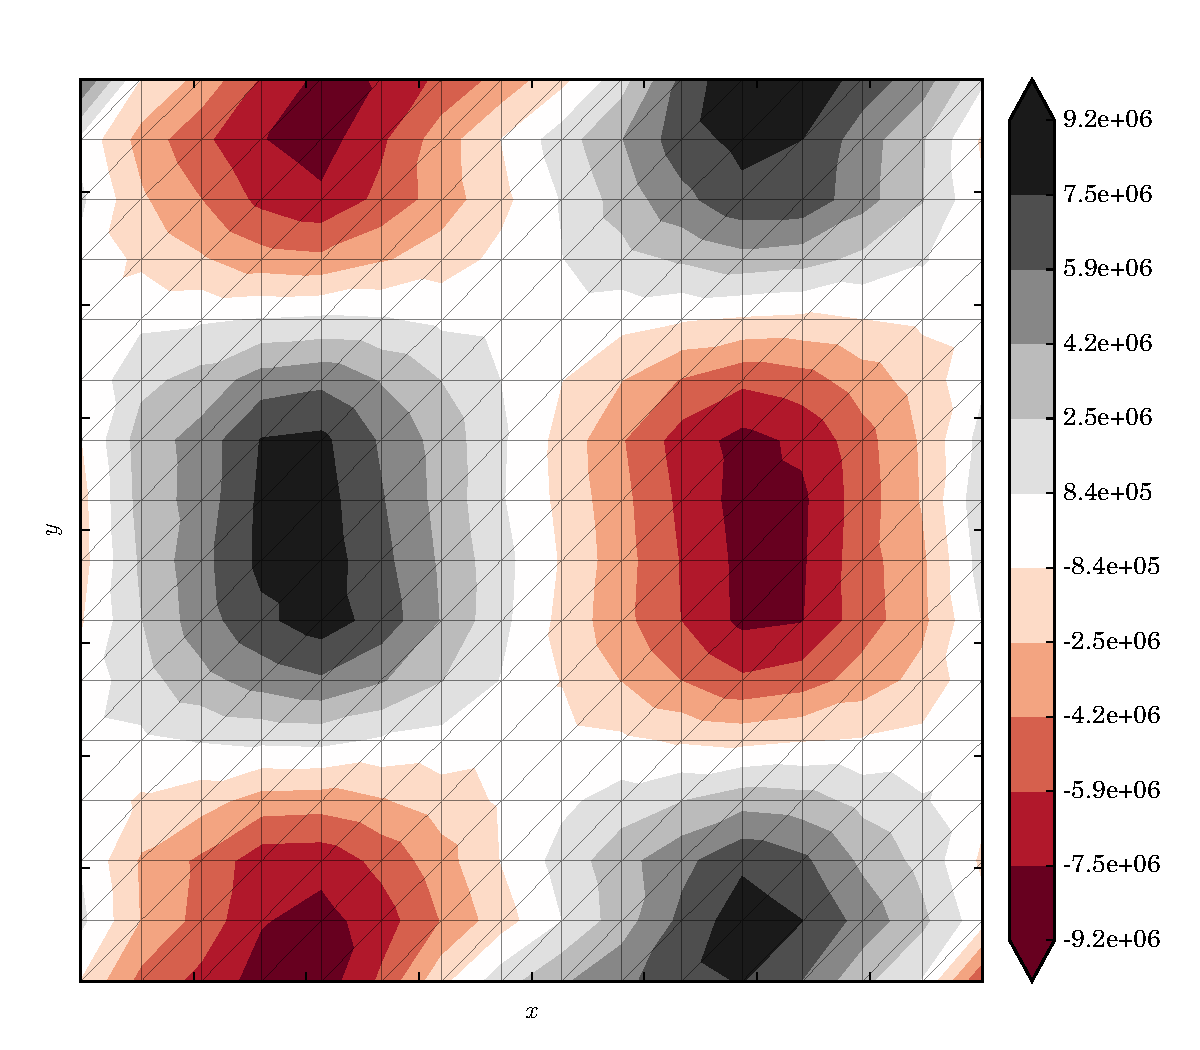
\includegraphics[width=\linewidth]{images/stress_balance/BP/N_ij.pdf}
  \caption{$N_{ij}$}
  \label{bp_N_ij}
  \end{subfigure}
  \begin{subfigure}[b]{0.3\linewidth}
    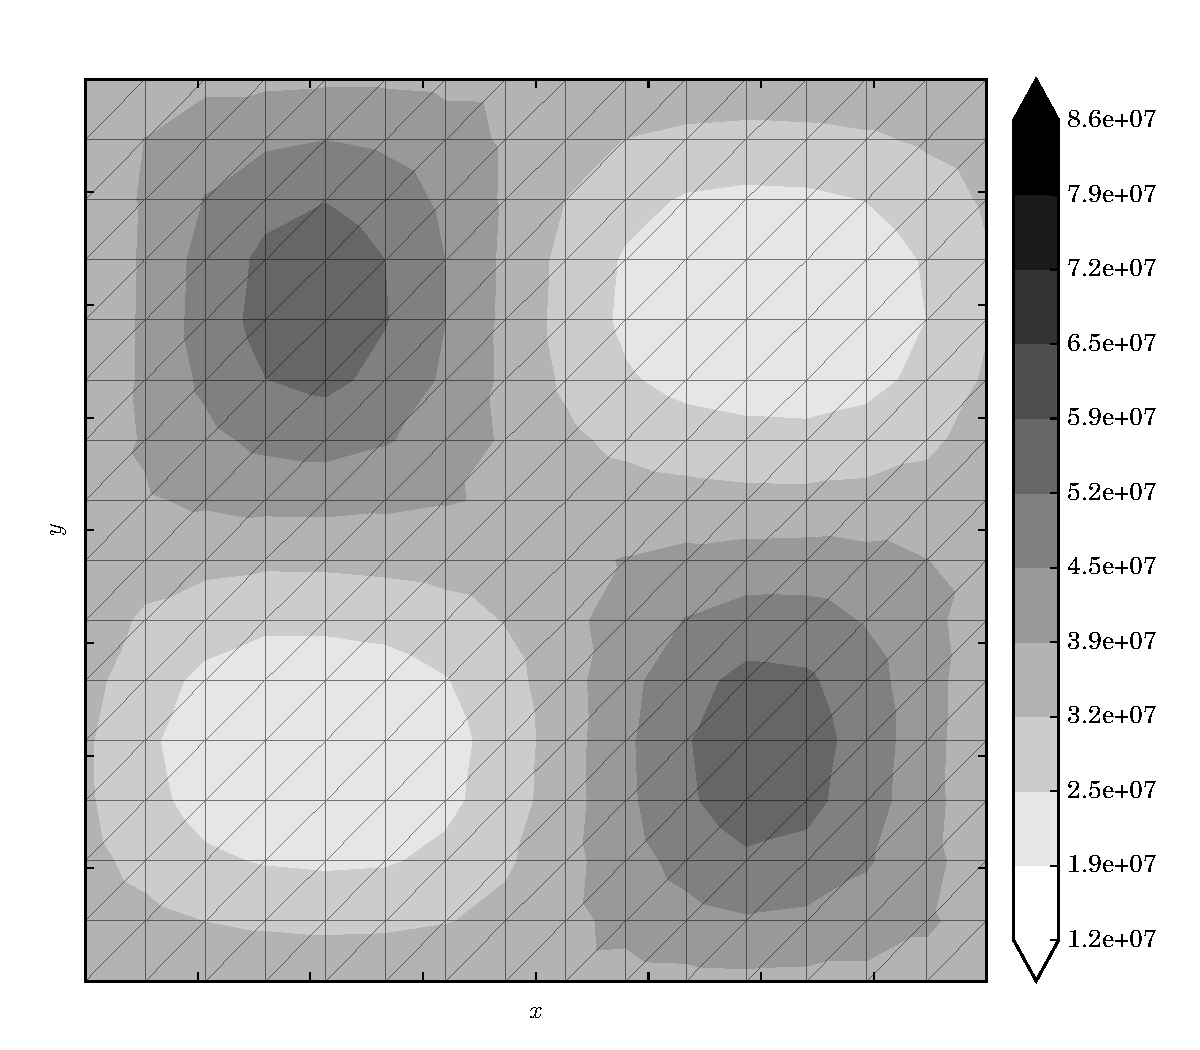
\includegraphics[width=\linewidth]{images/stress_balance/BP/N_iz.pdf}
  \caption{$N_{iz}$}
  \label{bp_N_iz}
  \end{subfigure}

  \begin{subfigure}[b]{0.3\linewidth}
    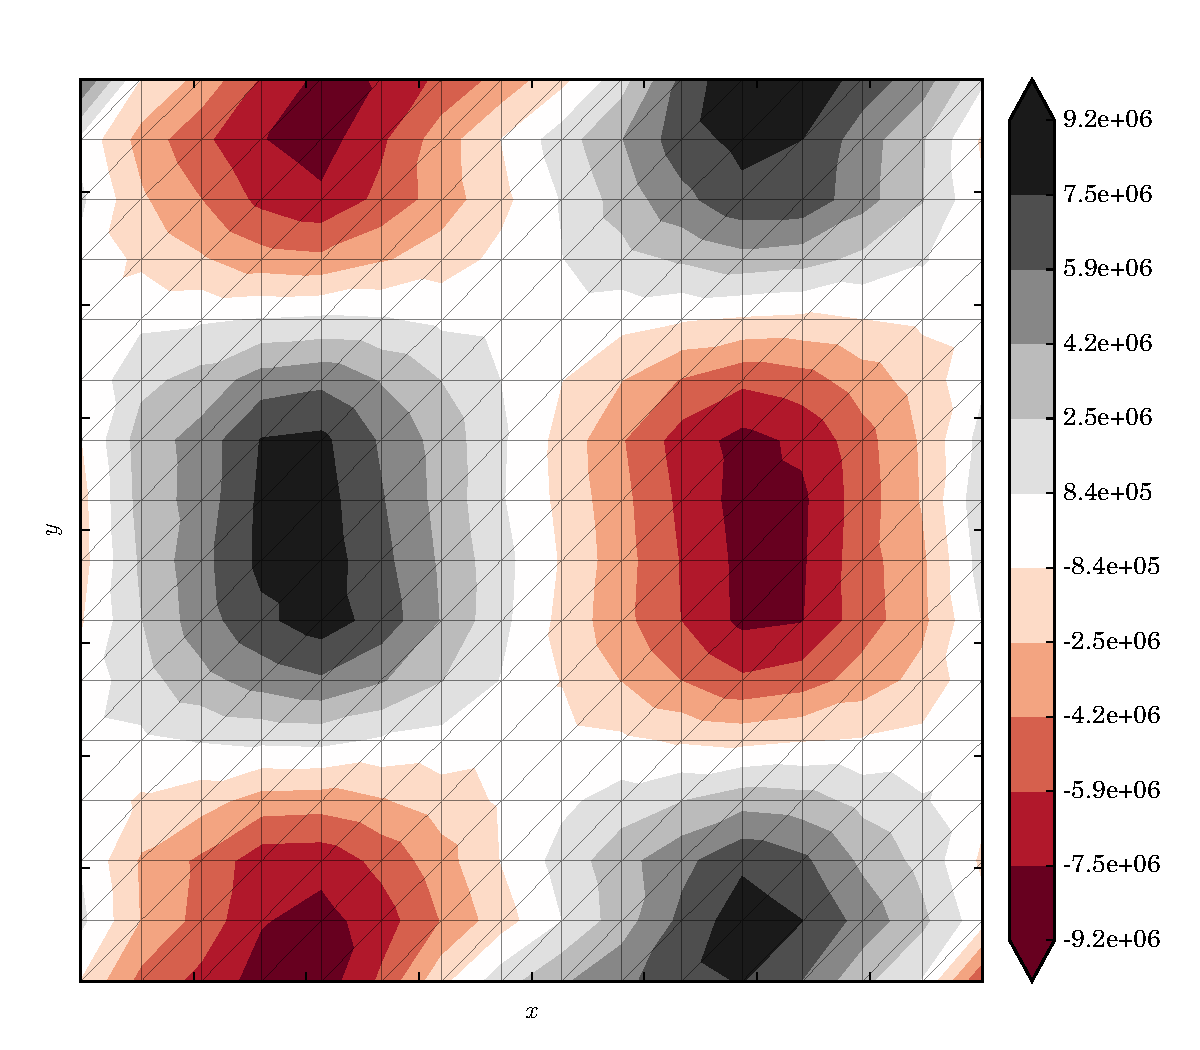
\includegraphics[width=\linewidth]{images/stress_balance/BP/N_ji.pdf}
  \caption{$N_{ji}$}
  \label{bp_N_ji}
  \end{subfigure}
  \begin{subfigure}[b]{0.3\linewidth}
    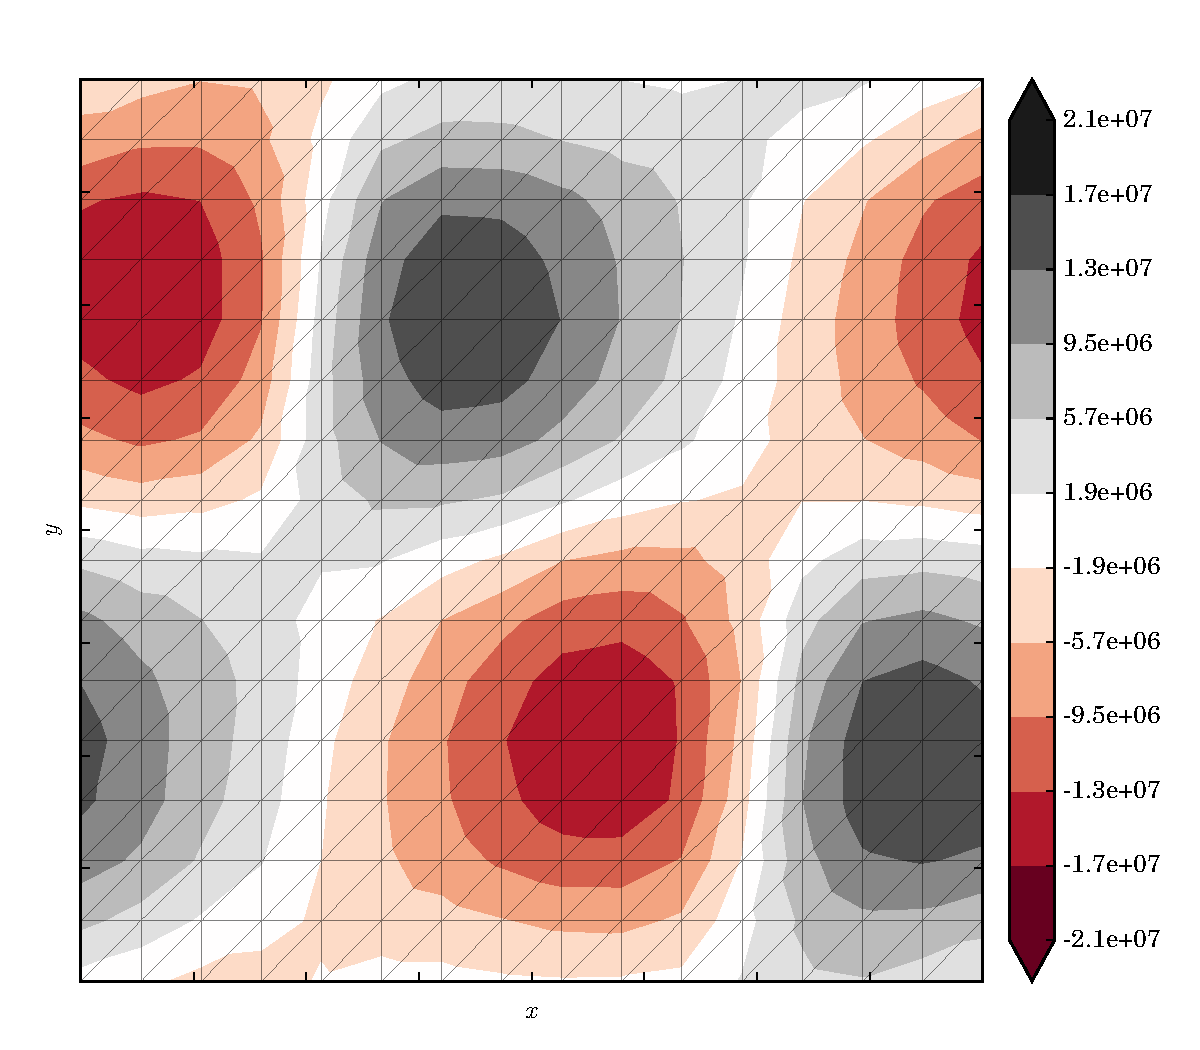
\includegraphics[width=\linewidth]{images/stress_balance/BP/N_jj.pdf}
  \caption{$N_{jj}$}
  \label{bp_N_jj}
  \end{subfigure}
  \begin{subfigure}[b]{0.3\linewidth}
    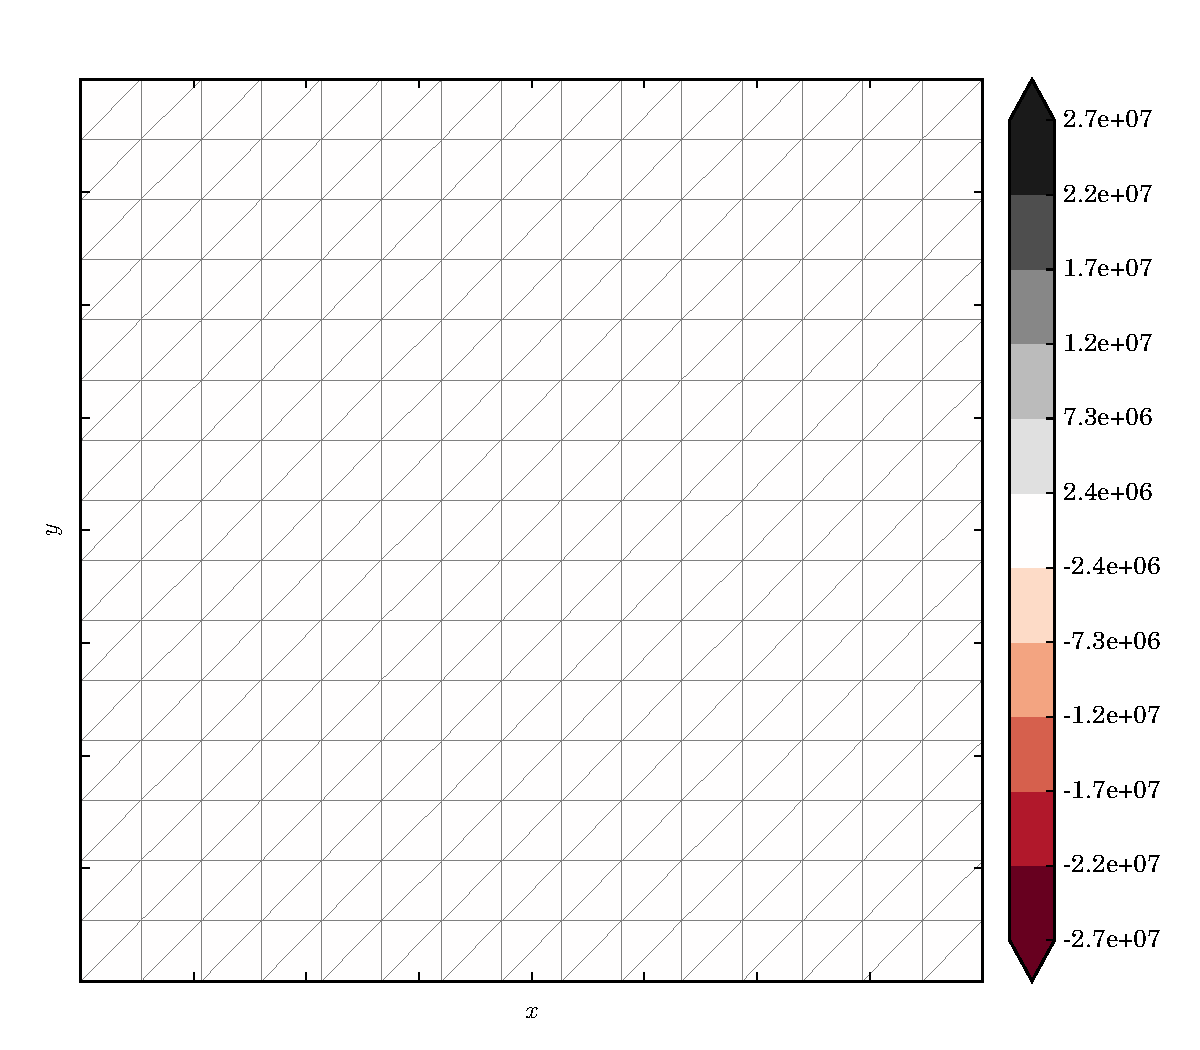
\includegraphics[width=\linewidth]{images/stress_balance/BP/N_jz.pdf}
  \caption{$N_{jz}$}
  \label{bp_N_jz}
  \end{subfigure}

  \begin{subfigure}[b]{0.3\linewidth}
    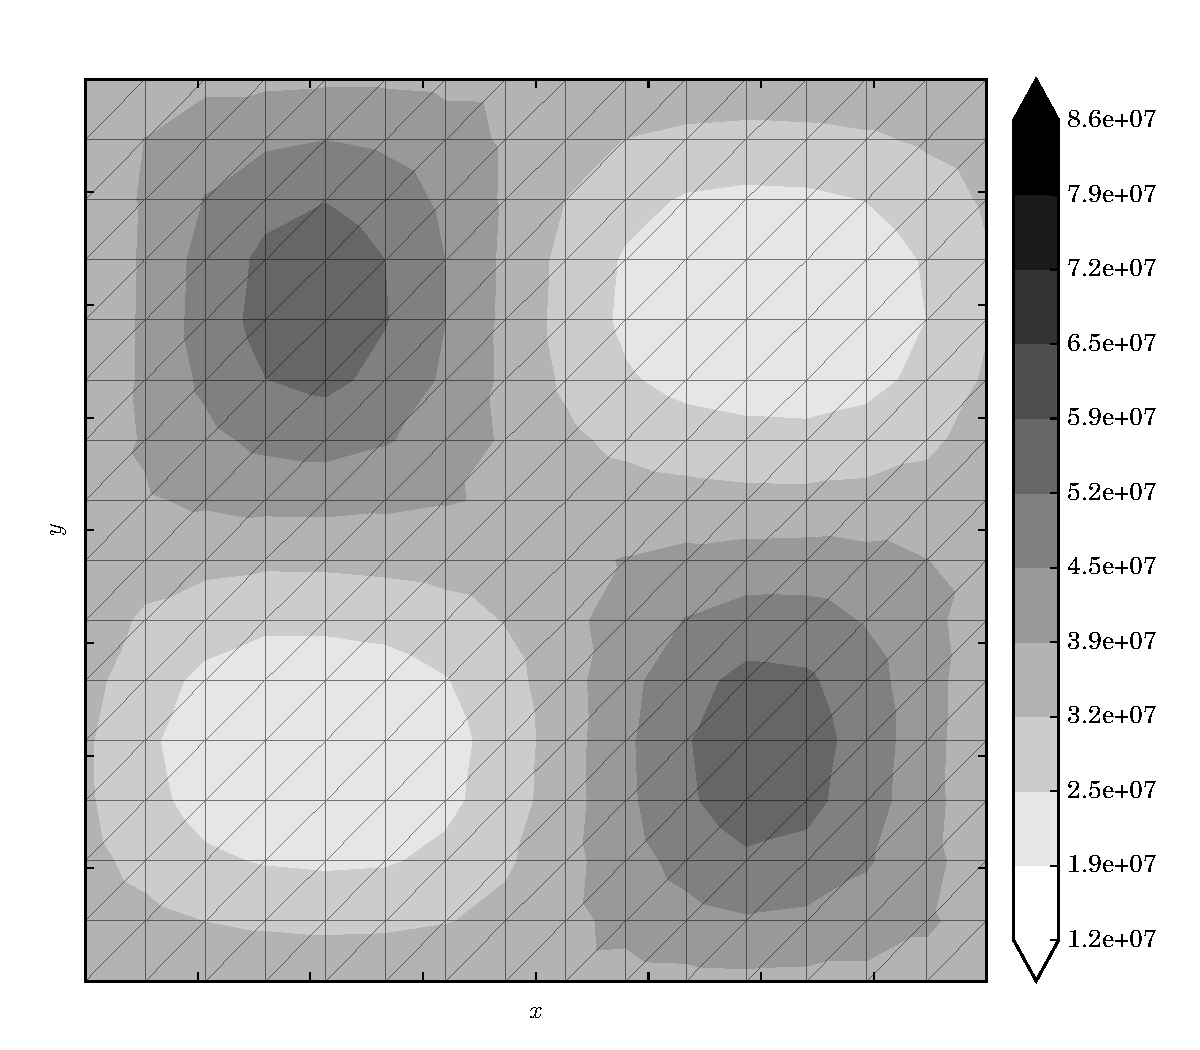
\includegraphics[width=\linewidth]{images/stress_balance/BP/N_zi.pdf}
  \caption{$N_{zi}$}
  \label{bp_N_zi}
  \end{subfigure}
  \begin{subfigure}[b]{0.3\linewidth}
    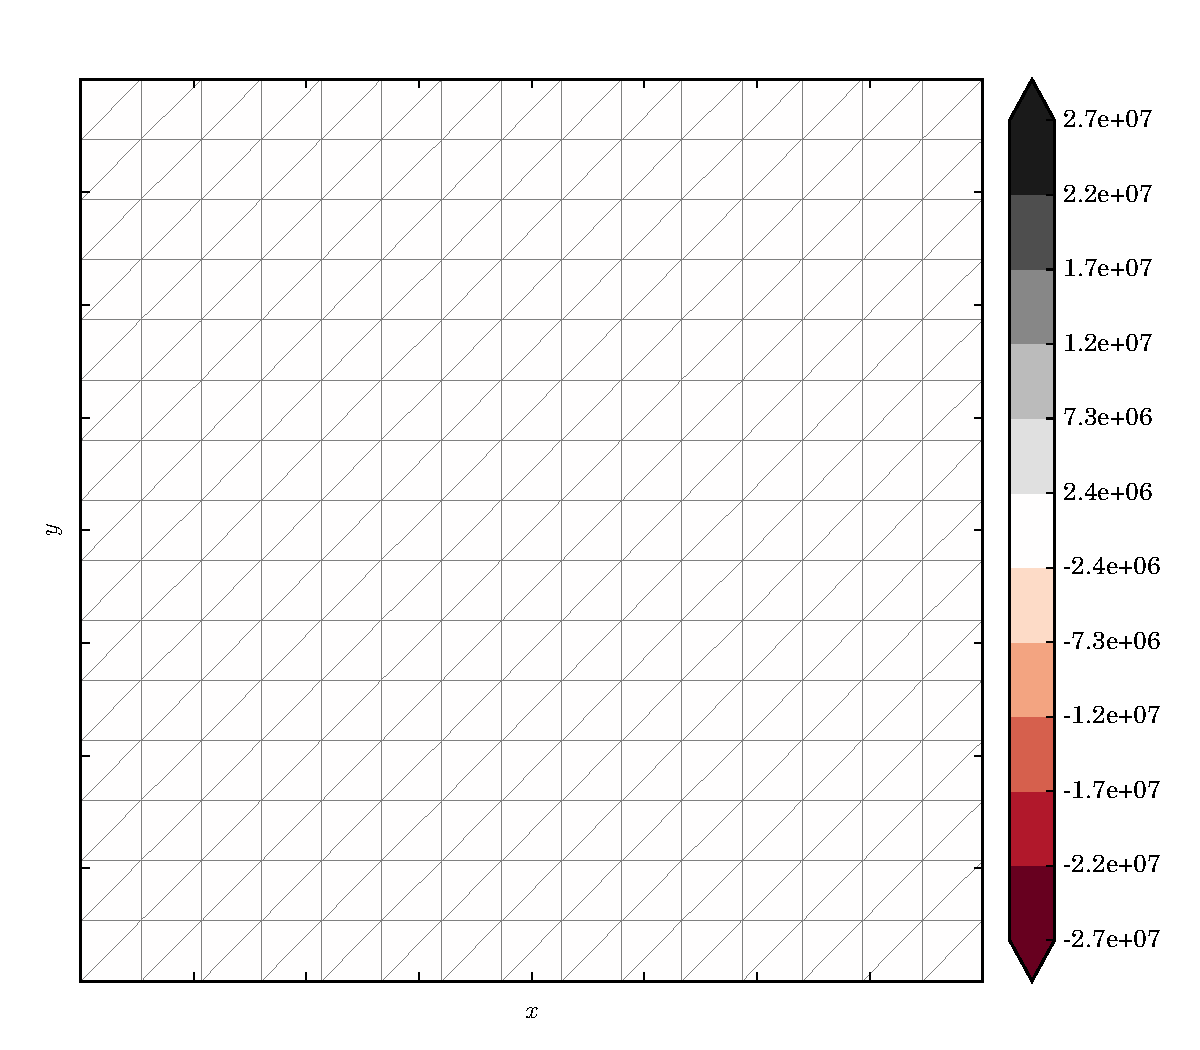
\includegraphics[width=\linewidth]{images/stress_balance/BP/N_zj.pdf}
  \caption{$N_{zj}$}
  \label{bp_N_zj}
  \end{subfigure}
  \begin{subfigure}[b]{0.3\linewidth}
    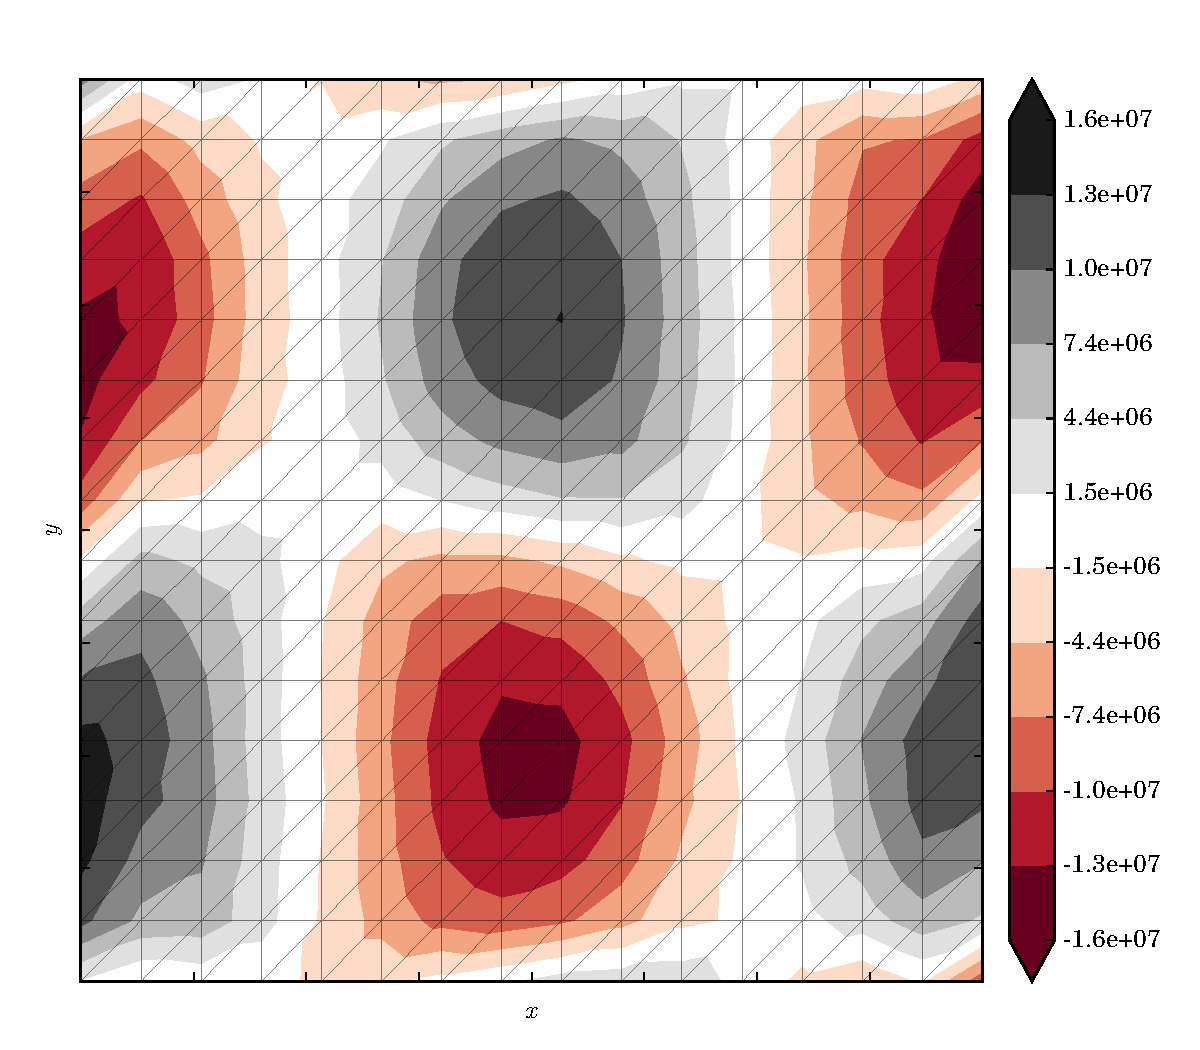
\includegraphics[width=\linewidth]{images/stress_balance/BP/N_zz.pdf}
  \caption{$N_{zz}$}
  \label{bp_N_zz}
  \end{subfigure}
 
  \caption[ISMIP-HOM first-order membrane stress]{First-order membrane stress $N_{kk}$.}

  \label{bp_membrane_stress}

\end{figure*}

%===============================================================================

\begin{figure*}
  
  \centering 
  
  \begin{subfigure}[b]{0.3\linewidth}
    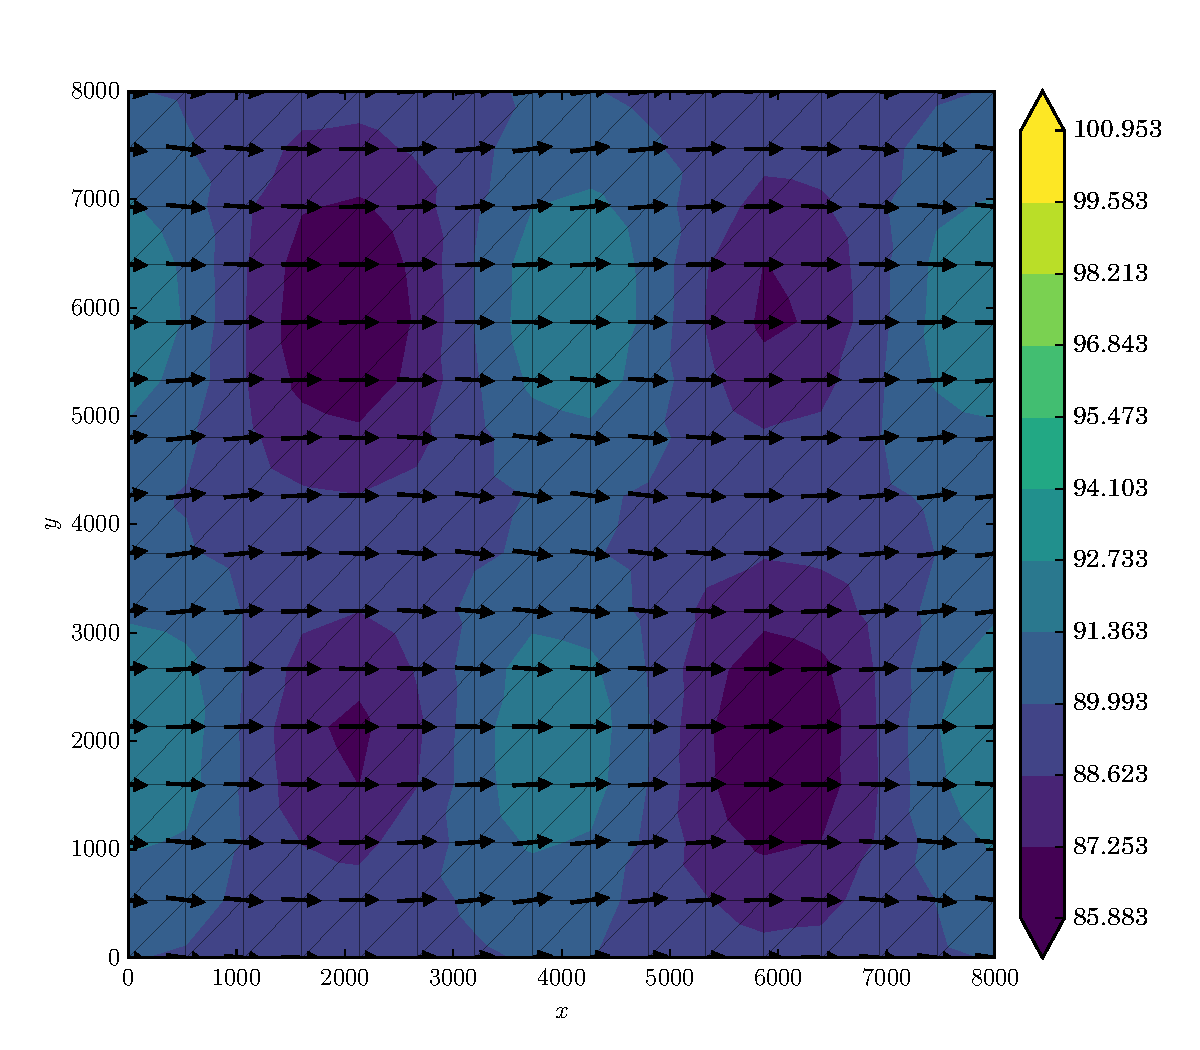
\includegraphics[width=\linewidth]{images/stress_balance/FS/U_mag.pdf}
  \caption{$\rankone{u}_S$}
  \label{fs_msb_U}
  \end{subfigure}
  \begin{subfigure}[b]{0.3\linewidth}
    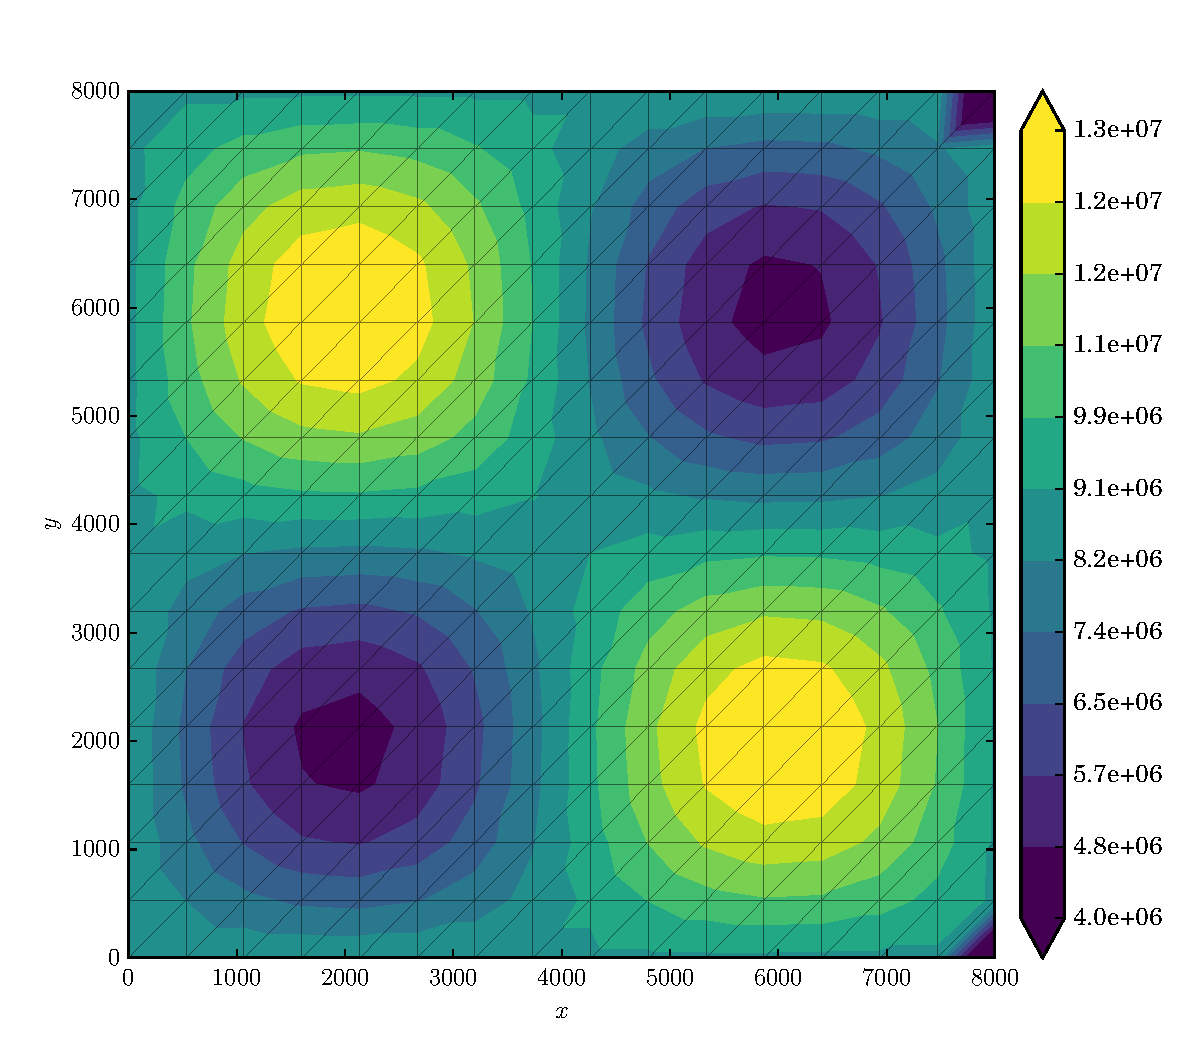
\includegraphics[width=\linewidth]{images/stress_balance/FS/p.pdf}
  \caption{$p |_B$}
  \label{fs_msb_p}
  \end{subfigure}

  \begin{subfigure}[b]{0.3\linewidth}
    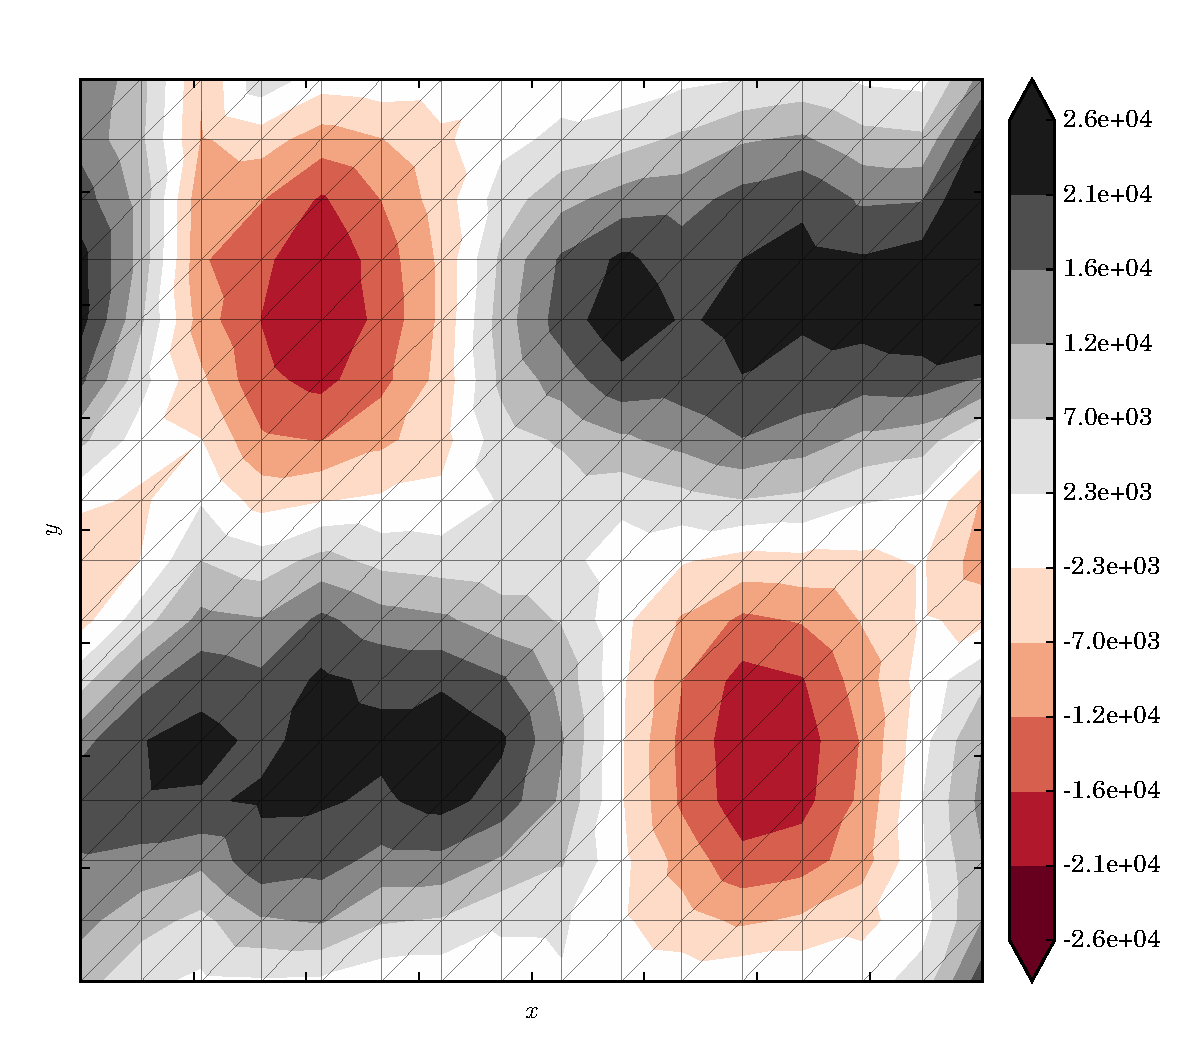
\includegraphics[width=\linewidth]{images/stress_balance/FS/M_ii.pdf}
  \caption{$M_{ii}$}
  \label{fs_M_ii}
  \end{subfigure}
  \begin{subfigure}[b]{0.3\linewidth}
    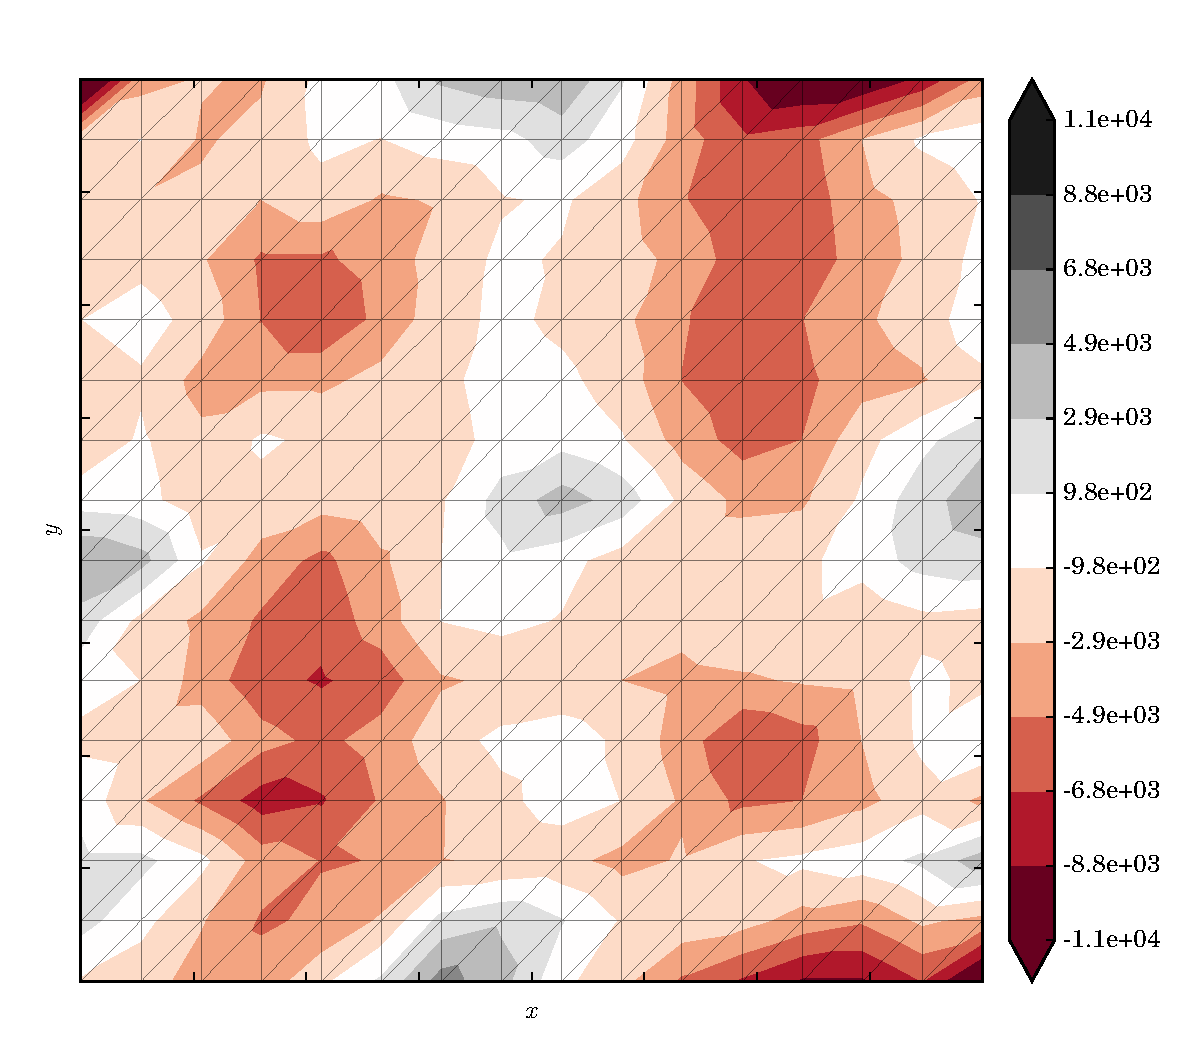
\includegraphics[width=\linewidth]{images/stress_balance/FS/M_ij.pdf}
  \caption{$M_{ij}$}
  \label{fs_M_ij}
  \end{subfigure}
  \begin{subfigure}[b]{0.3\linewidth}
    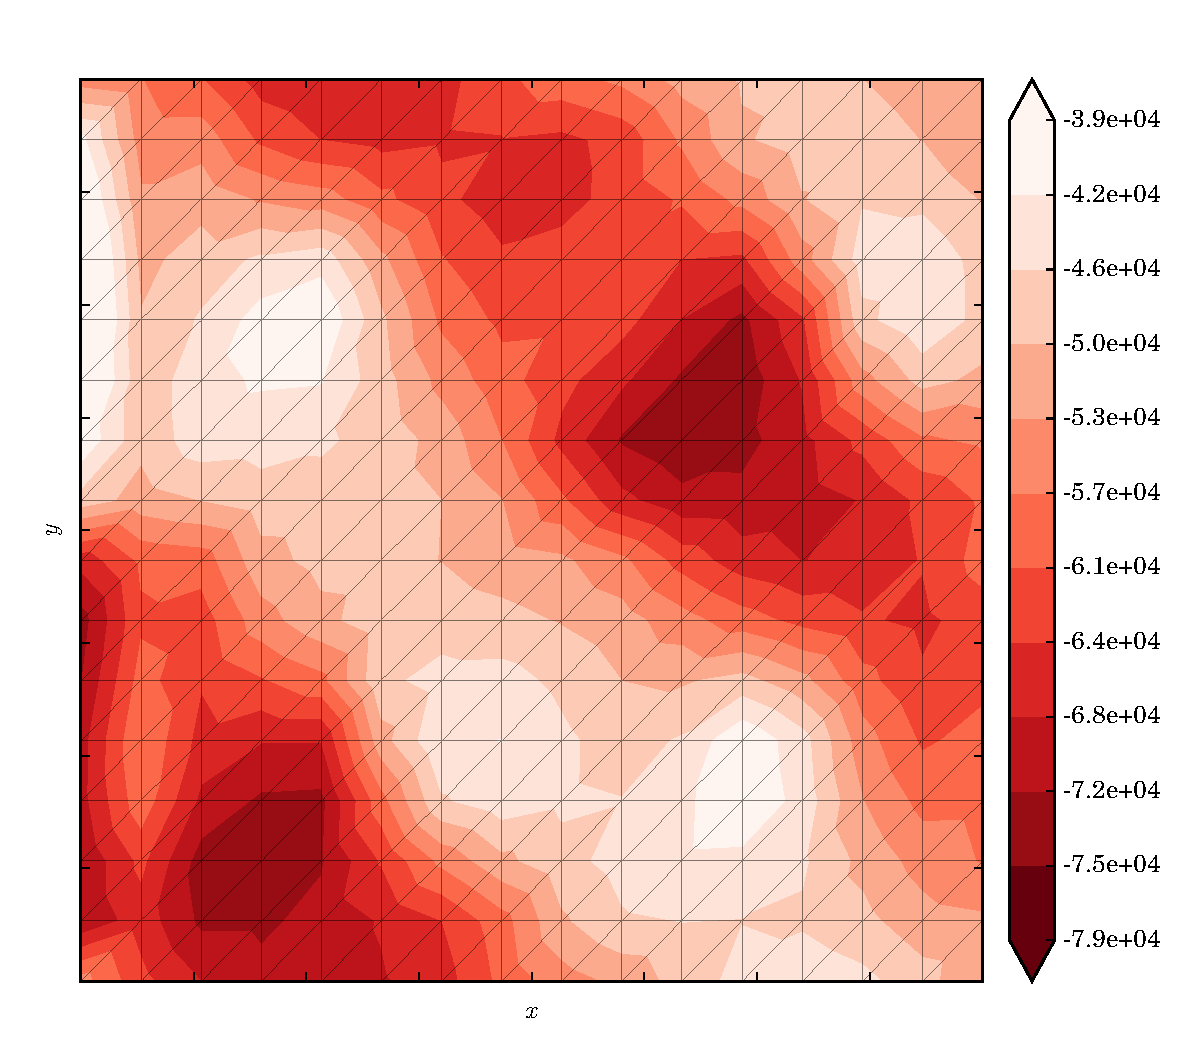
\includegraphics[width=\linewidth]{images/stress_balance/FS/M_iz.pdf}
  \caption{$M_{iz}$}
  \label{fs_M_iz}
  \end{subfigure}

  \begin{subfigure}[b]{0.3\linewidth}
    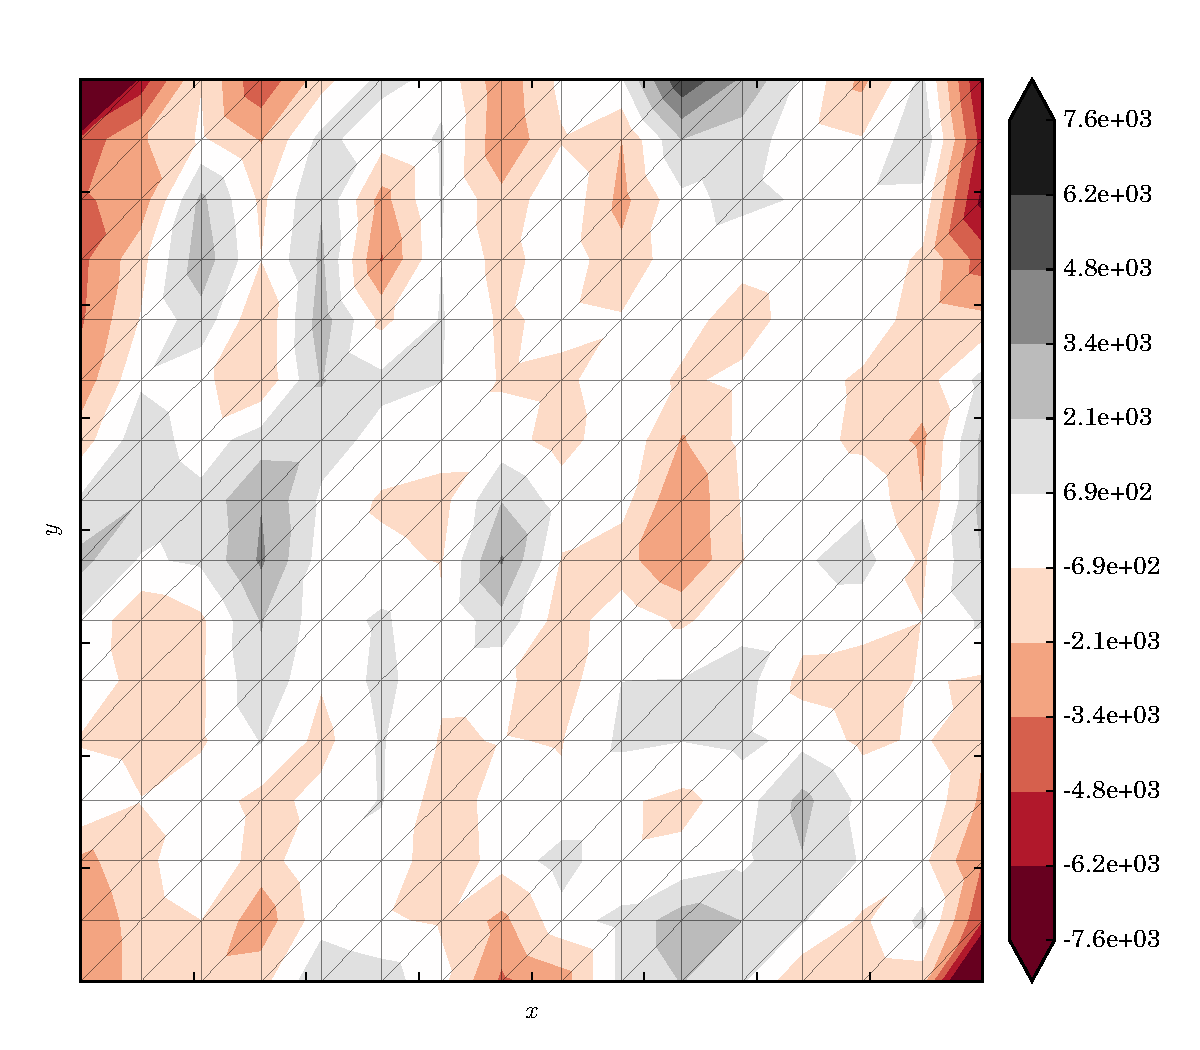
\includegraphics[width=\linewidth]{images/stress_balance/FS/M_ji.pdf}
  \caption{$M_{ji}$}
  \label{fs_M_ji}
  \end{subfigure}
  \begin{subfigure}[b]{0.3\linewidth}
    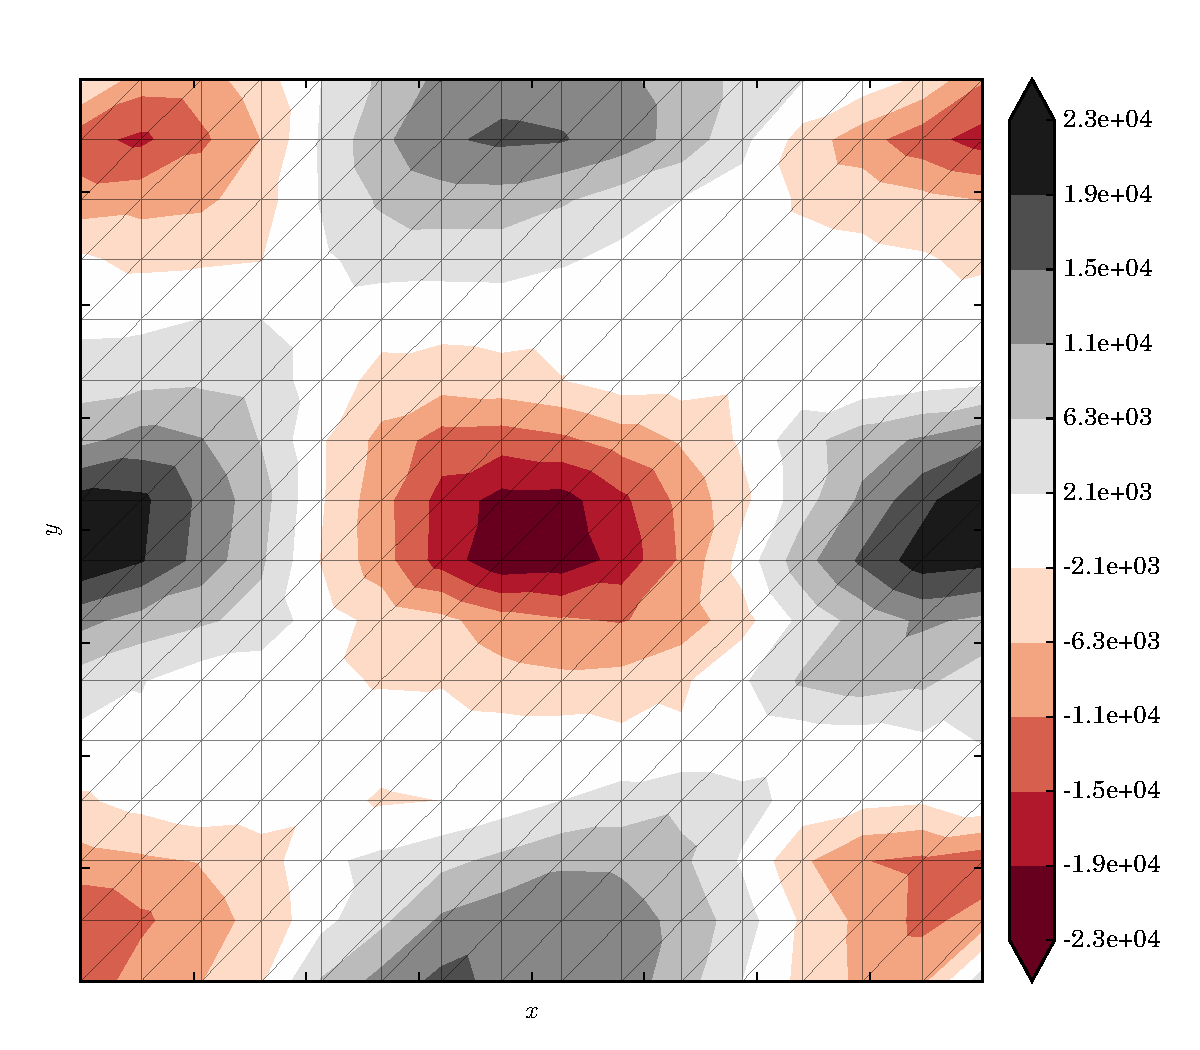
\includegraphics[width=\linewidth]{images/stress_balance/FS/M_jj.pdf}
  \caption{$M_{jj}$}
  \label{fs_M_jj}
  \end{subfigure}
  \begin{subfigure}[b]{0.3\linewidth}
    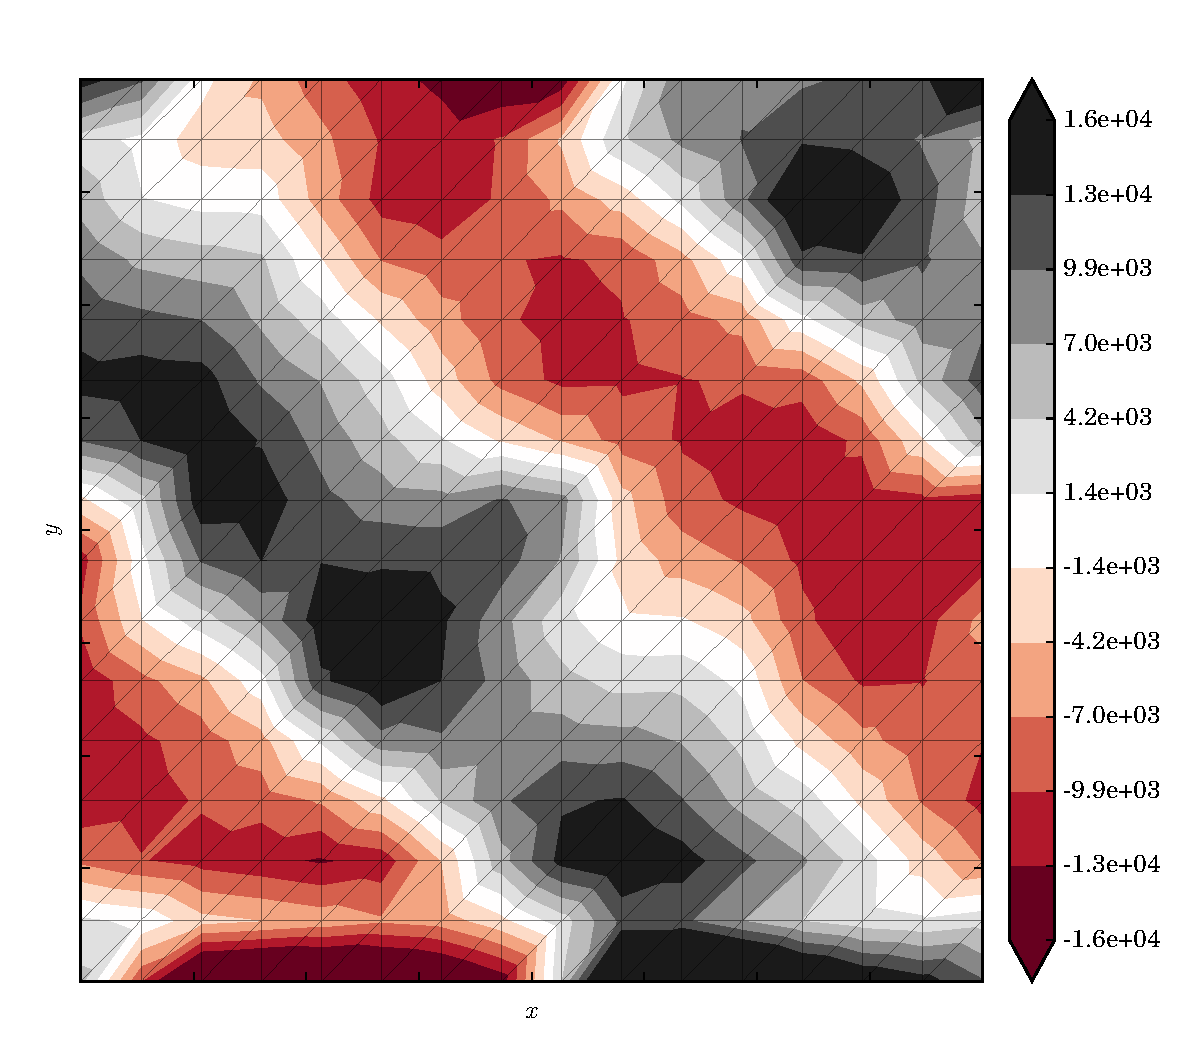
\includegraphics[width=\linewidth]{images/stress_balance/FS/M_jz.pdf}
  \caption{$M_{jz}$}
  \label{fs_M_jz}
  \end{subfigure}

  \begin{subfigure}[b]{0.3\linewidth}
    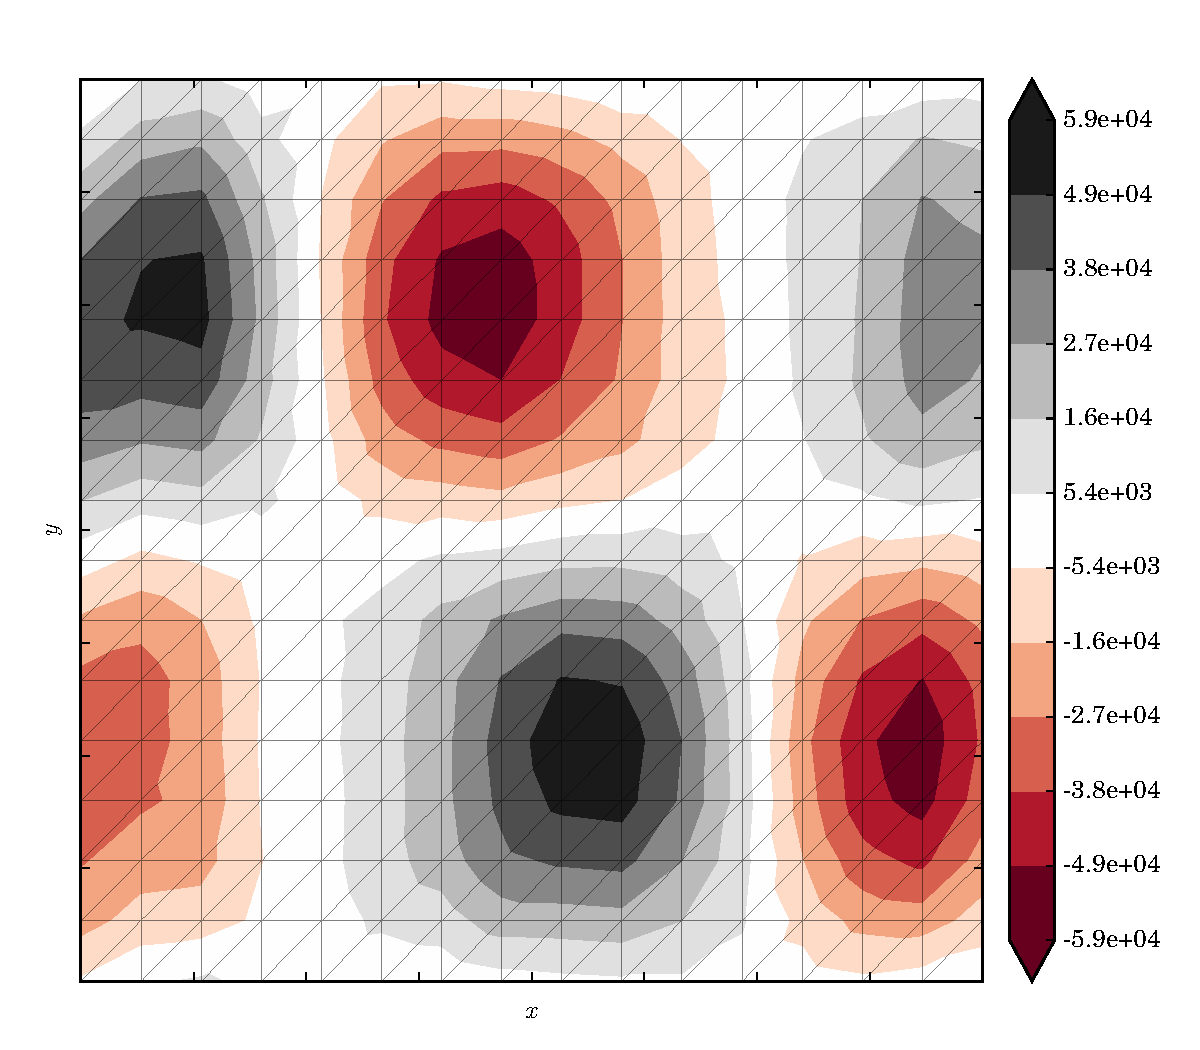
\includegraphics[width=\linewidth]{images/stress_balance/FS/M_zi.pdf}
  \caption{$M_{zi}$}
  \label{fs_M_zi}
  \end{subfigure}
  \begin{subfigure}[b]{0.3\linewidth}
    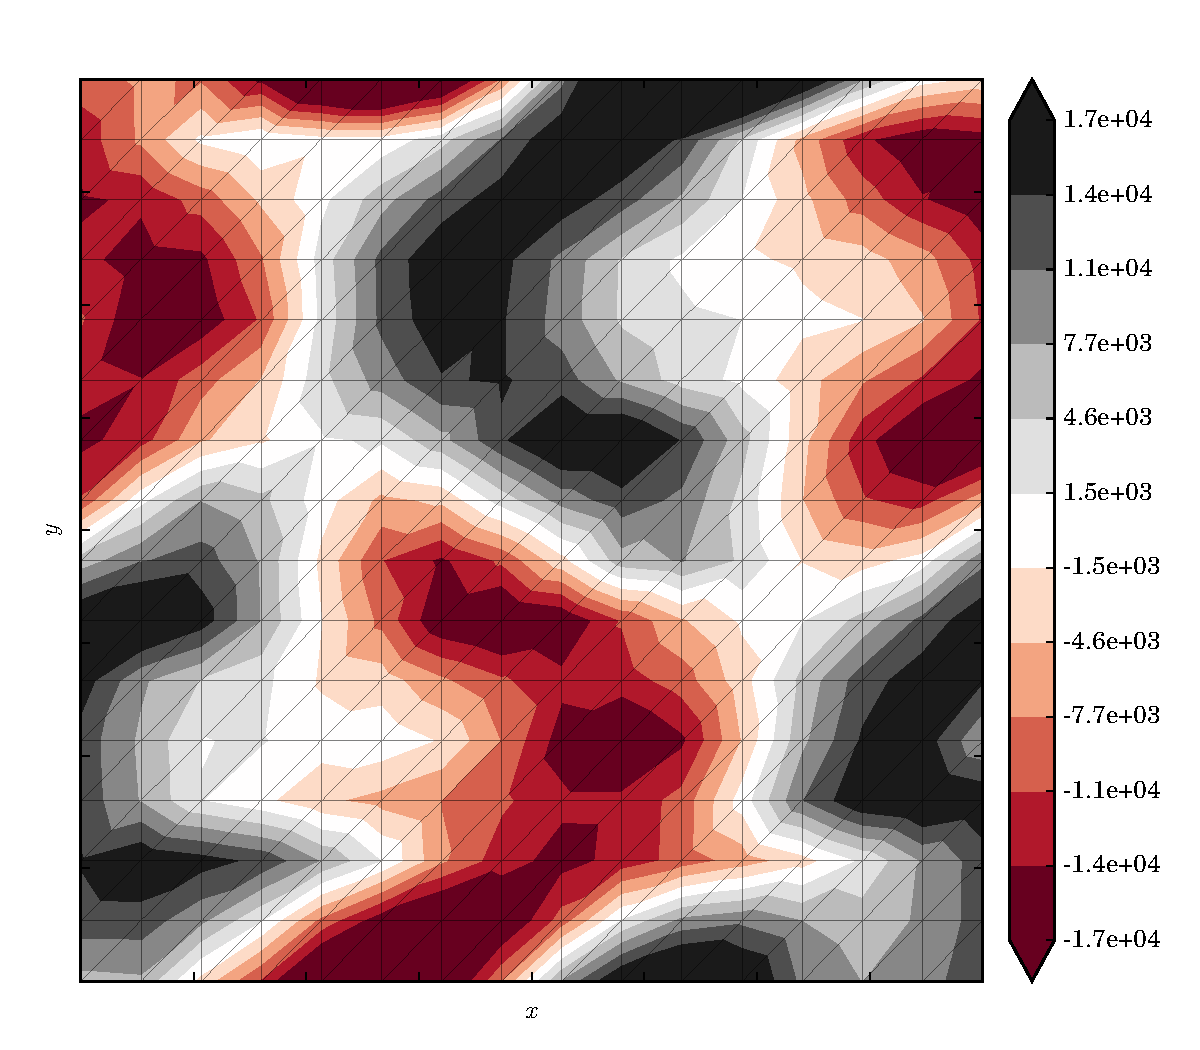
\includegraphics[width=\linewidth]{images/stress_balance/FS/M_zj.pdf}
  \caption{$M_{zj}$}
  \label{fs_M_zj}
  \end{subfigure}
  \begin{subfigure}[b]{0.3\linewidth}
    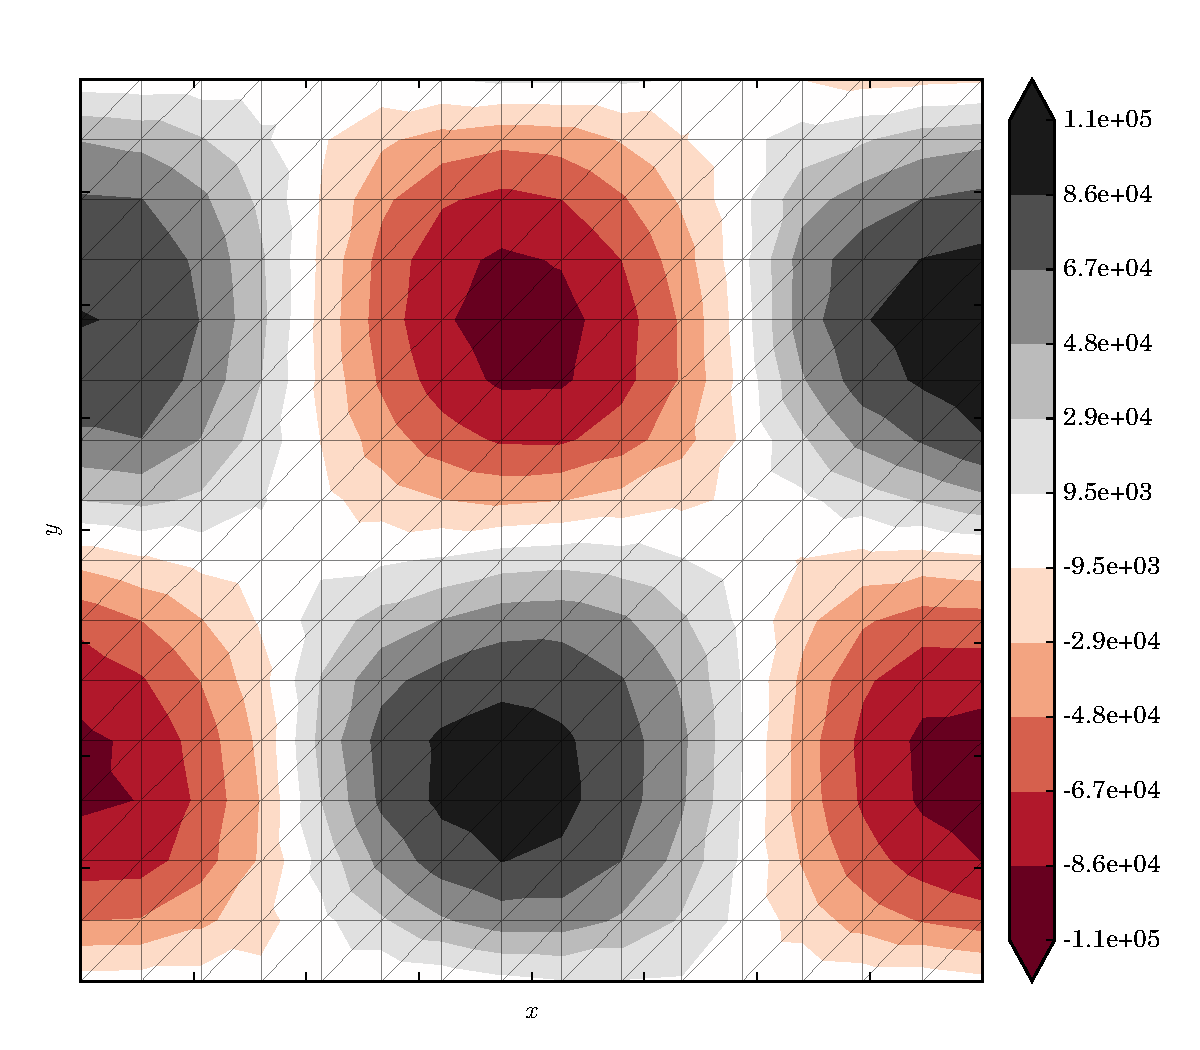
\includegraphics[width=\linewidth]{images/stress_balance/FS/M_zz.pdf}
  \caption{$M_{zz}$}
  \label{fs_M_zz}
  \end{subfigure}
 
  \caption[ISMIP-HOM full-Stokes membrane stress balance]{Full-Stokes membrane stress balance $M_{kk}$.}

  \label{fs_membrane_stress_balance}

\end{figure*}

%===============================================================================

\begin{figure*}
  
  \centering 
  
  \begin{subfigure}[b]{0.3\linewidth}
    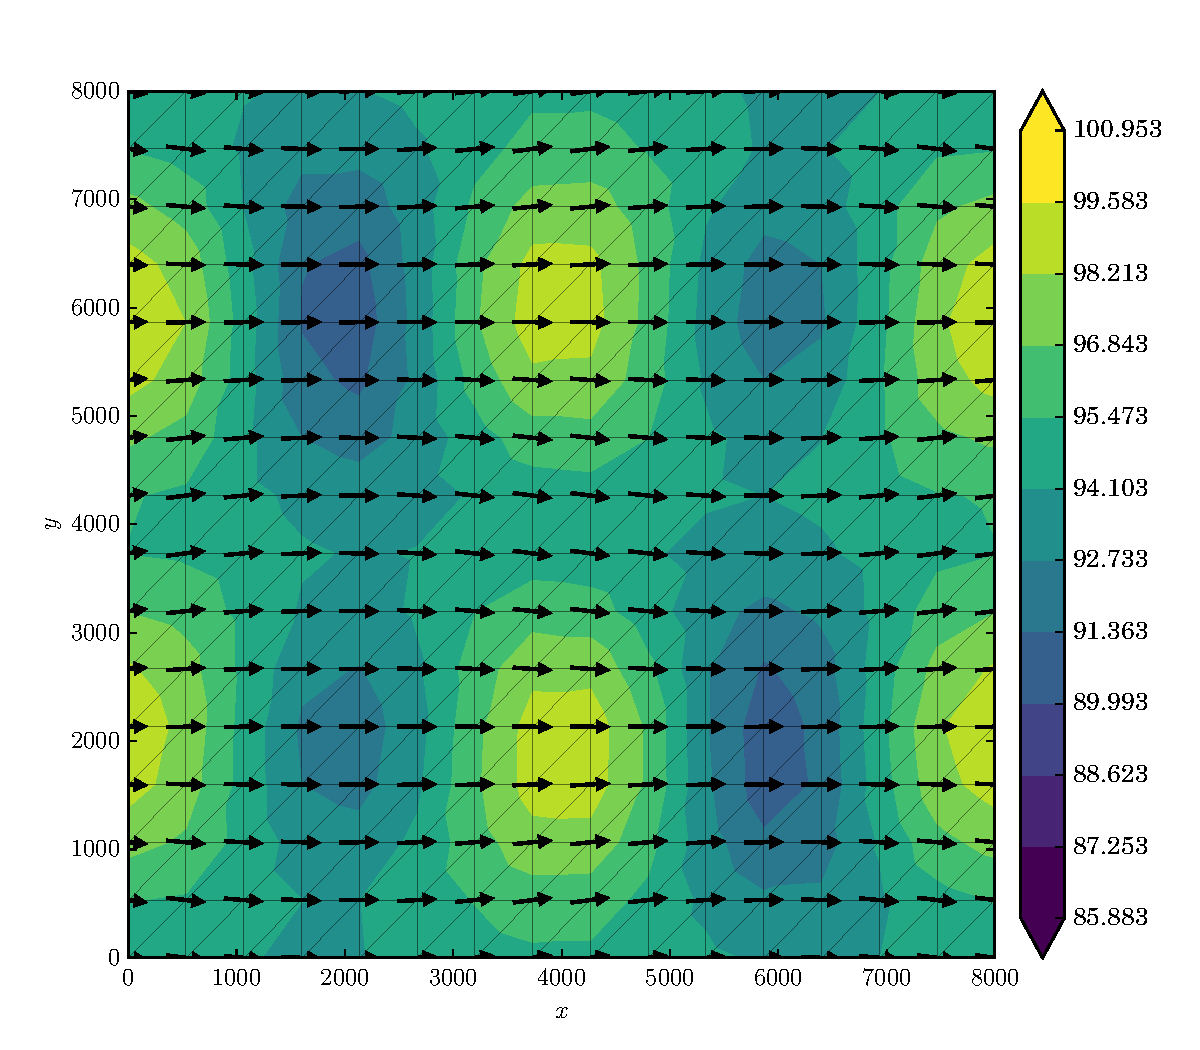
\includegraphics[width=\linewidth]{images/stress_balance/RS/U_mag.pdf}
  \caption{$\rankone{u}_S$}
  \label{rs_msb_U}
  \end{subfigure}
  \begin{subfigure}[b]{0.3\linewidth}
    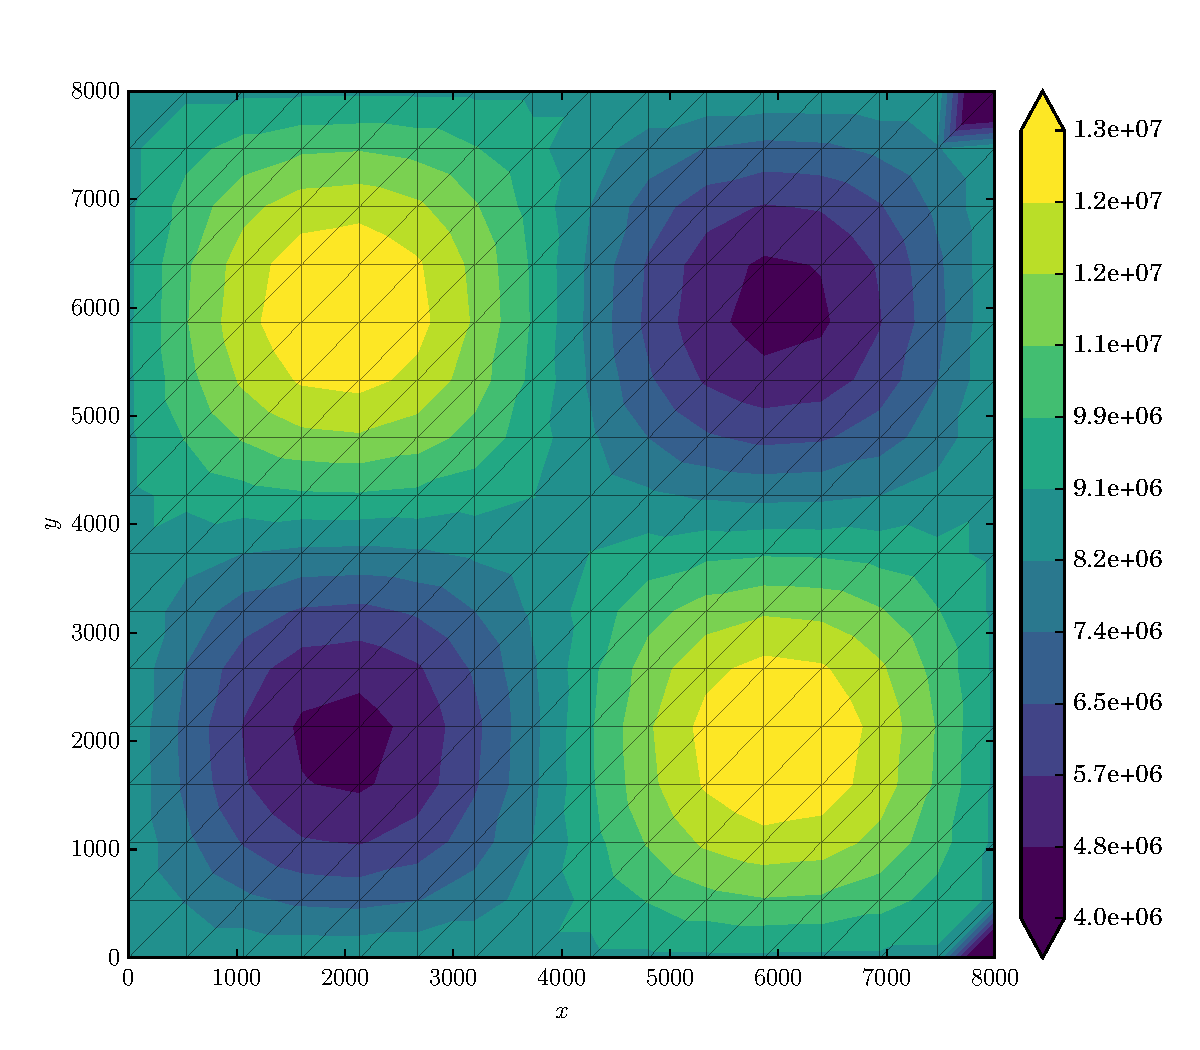
\includegraphics[width=\linewidth]{images/stress_balance/RS/p.pdf}
  \caption{$p |_B$}
  \label{rs_msb_p}
  \end{subfigure}

  \begin{subfigure}[b]{0.3\linewidth}
    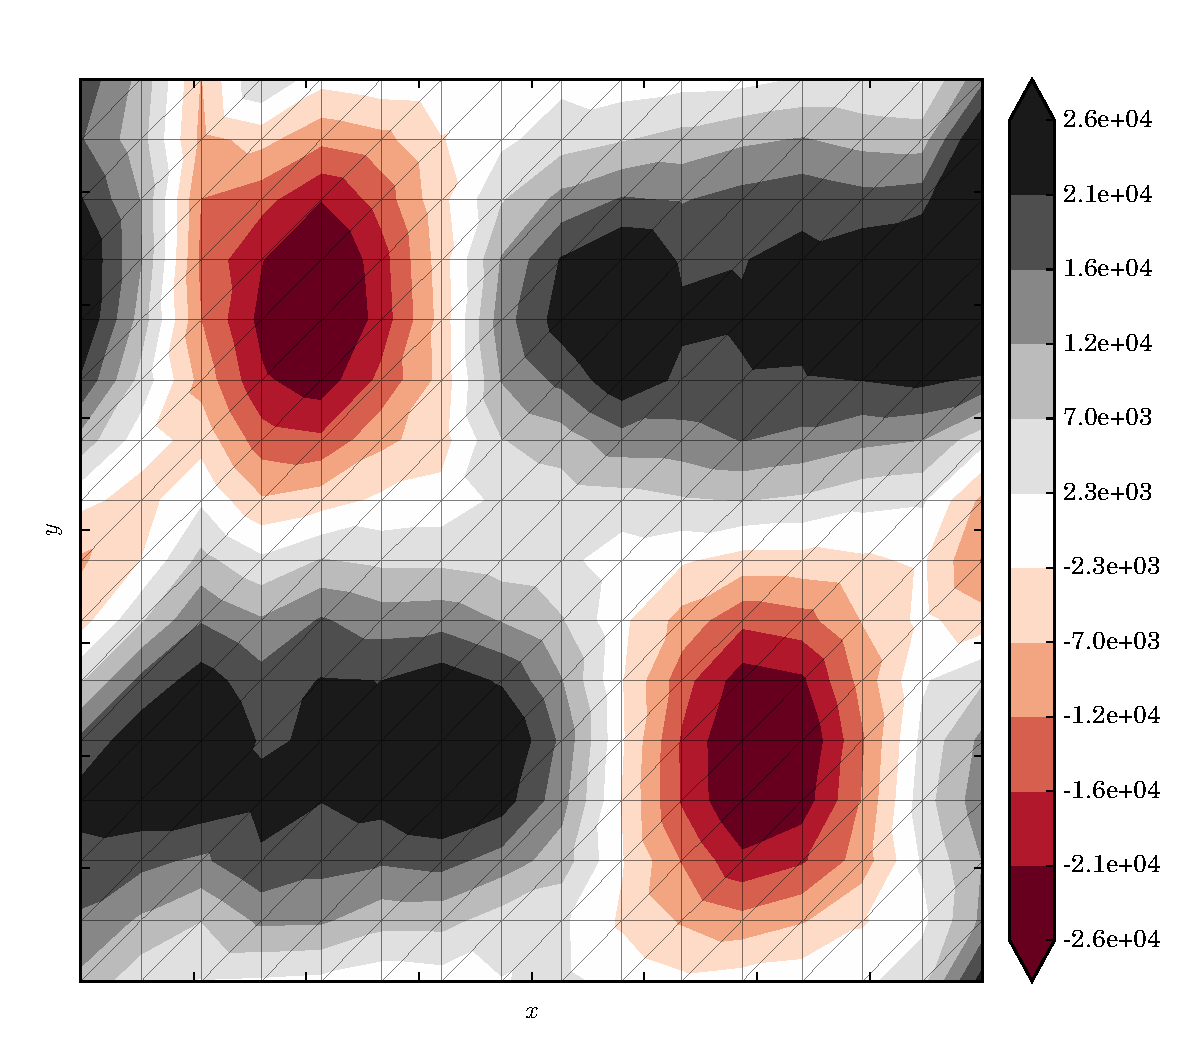
\includegraphics[width=\linewidth]{images/stress_balance/RS/M_ii.pdf}
  \caption{$M_{ii}$}
  \label{rs_M_ii}
  \end{subfigure}
  \begin{subfigure}[b]{0.3\linewidth}
    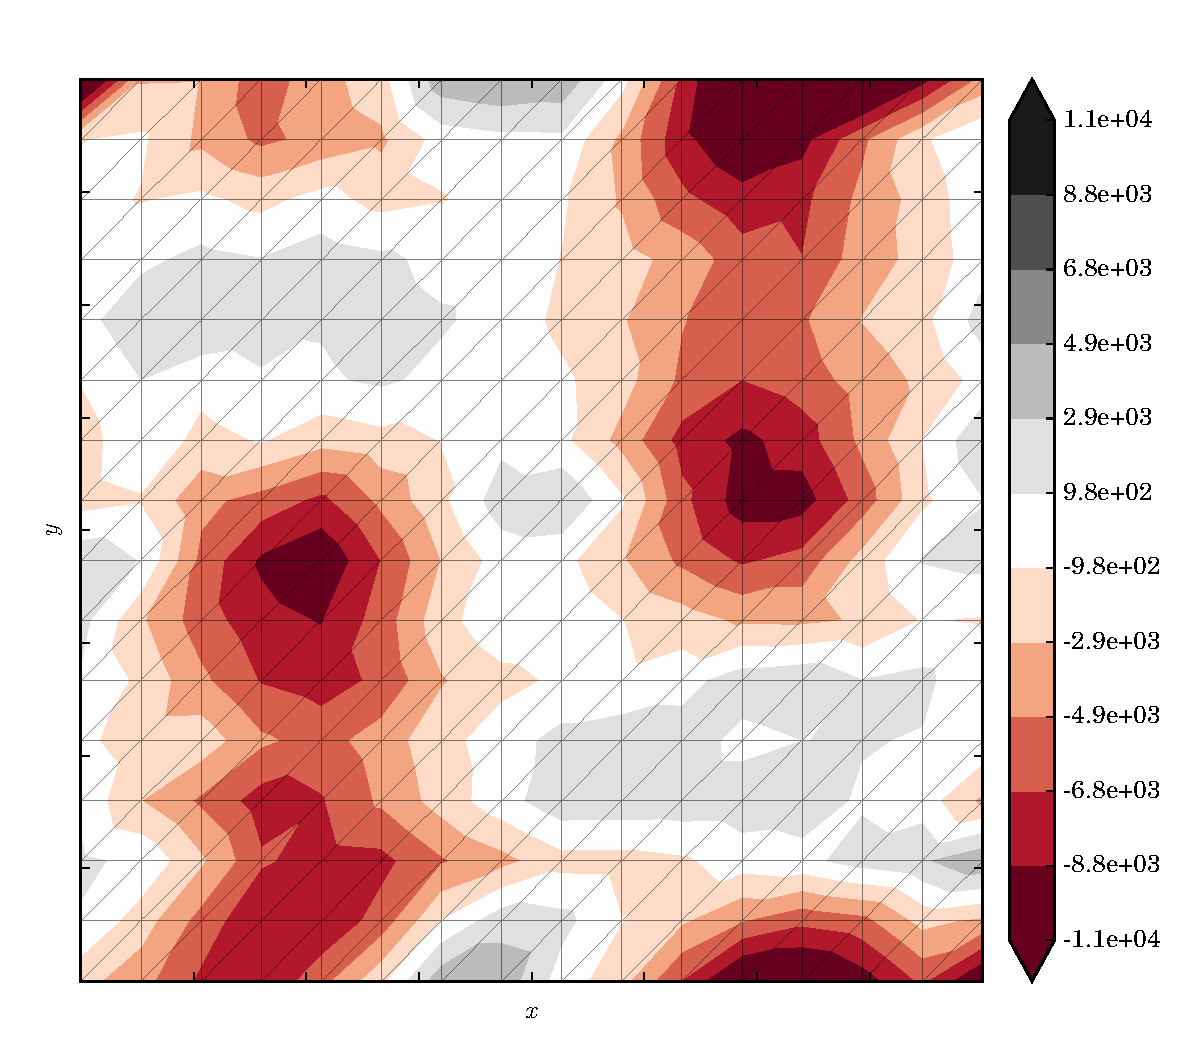
\includegraphics[width=\linewidth]{images/stress_balance/RS/M_ij.pdf}
  \caption{$M_{ij}$}
  \label{rs_M_ij}
  \end{subfigure}
  \begin{subfigure}[b]{0.3\linewidth}
    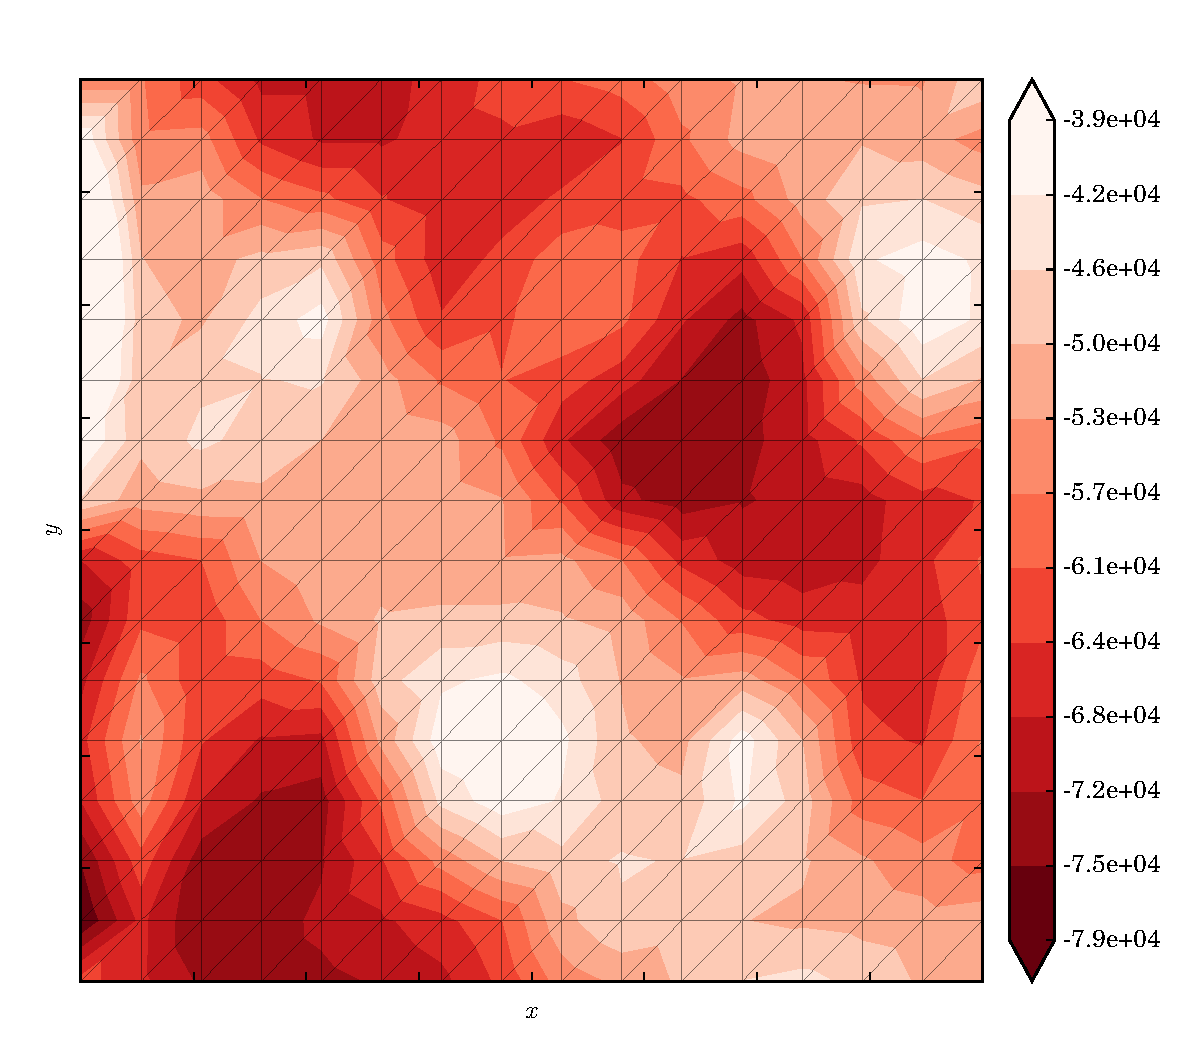
\includegraphics[width=\linewidth]{images/stress_balance/RS/M_iz.pdf}
  \caption{$M_{iz}$}
  \label{rs_M_iz}
  \end{subfigure}

  \begin{subfigure}[b]{0.3\linewidth}
    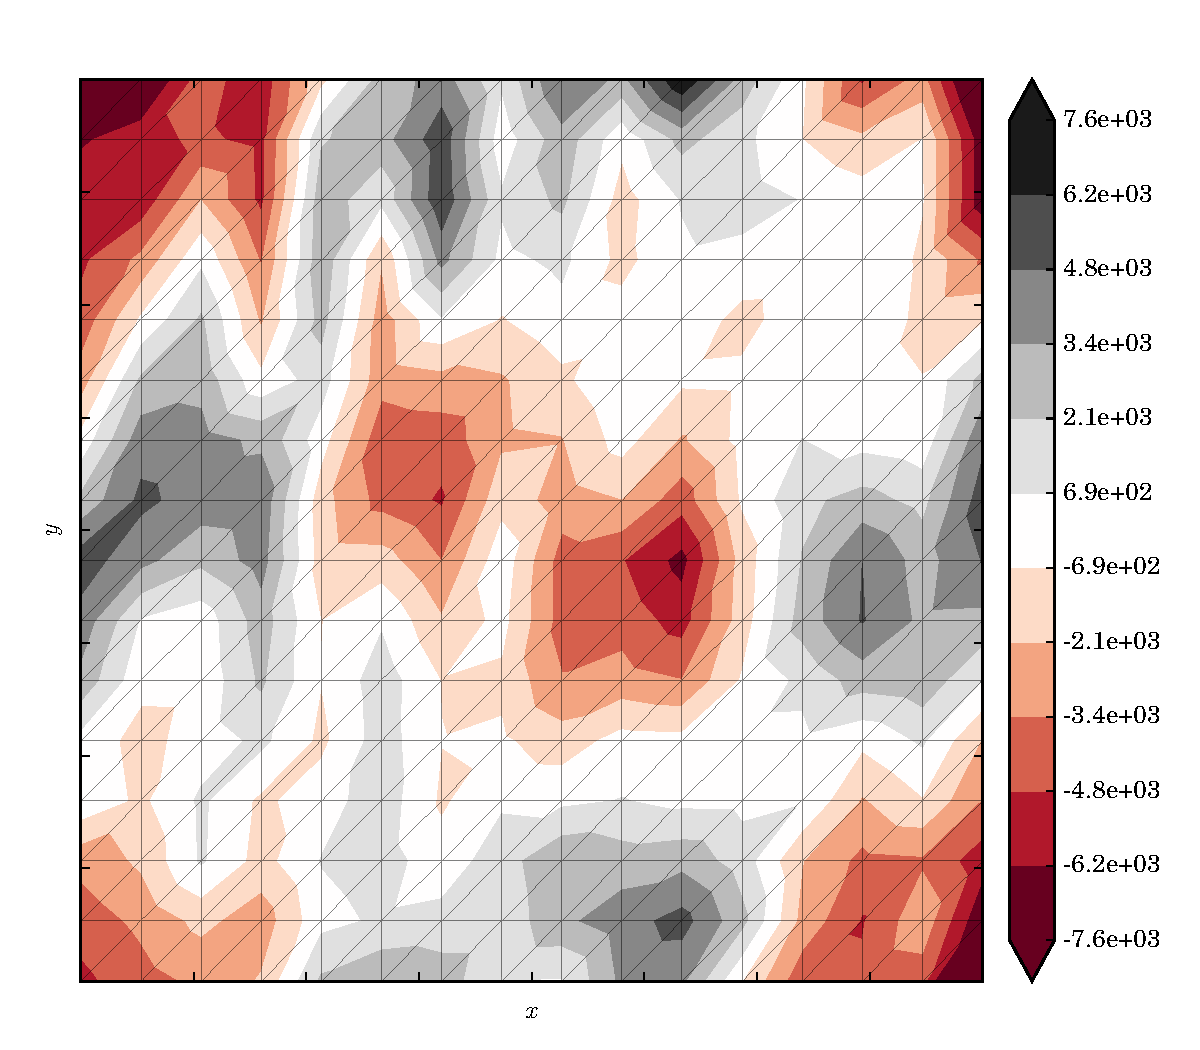
\includegraphics[width=\linewidth]{images/stress_balance/RS/M_ji.pdf}
  \caption{$M_{ji}$}
  \label{rs_M_ji}
  \end{subfigure}
  \begin{subfigure}[b]{0.3\linewidth}
    \includegraphics[width=\linewidth]{images/stress_balance/RS/M_jj.pdf}
  \caption{$M_{jj}$}
  \label{rs_M_jj}
  \end{subfigure}
  \begin{subfigure}[b]{0.3\linewidth}
    \includegraphics[width=\linewidth]{images/stress_balance/RS/M_jz.pdf}
  \caption{$M_{jz}$}
  \label{rs_M_jz}
  \end{subfigure}

  \begin{subfigure}[b]{0.3\linewidth}
    \includegraphics[width=\linewidth]{images/stress_balance/RS/M_zi.pdf}
  \caption{$M_{zi}$}
  \label{rs_M_zi}
  \end{subfigure}
  \begin{subfigure}[b]{0.3\linewidth}
    \includegraphics[width=\linewidth]{images/stress_balance/RS/M_zj.pdf}
  \caption{$M_{zj}$}
  \label{rs_M_zj}
  \end{subfigure}
  \begin{subfigure}[b]{0.3\linewidth}
    \includegraphics[width=\linewidth]{images/stress_balance/RS/M_zz.pdf}
  \caption{$M_{zz}$}
  \label{rs_M_zz}
  \end{subfigure}
 
  \caption[ISMIP-HOM reformulated-Stokes membrane stress balance]{Reformulated-Stokes membrane stress balance $M_{kk}$.}

  \label{rs_membrane_stress_balance}

\end{figure*}

%===============================================================================

\begin{figure*}
  
  \centering 

  \begin{subfigure}[b]{0.3\linewidth}
    \includegraphics[width=\linewidth]{images/stress_balance/BP/U_mag.pdf}
  \caption{$\rankone{u}_S$}
  \label{bp_msb_U}
  \end{subfigure}
  \begin{subfigure}[b]{0.3\linewidth}
    \includegraphics[width=\linewidth]{images/stress_balance/BP/p.pdf}
  \caption{$p |_B$}
  \label{bp_msb_p}
  \end{subfigure}

  \begin{subfigure}[b]{0.3\linewidth}
    \includegraphics[width=\linewidth]{images/stress_balance/BP/M_ii.pdf}
  \caption{$M_{ii}$}
  \label{bp_M_ii}
  \end{subfigure}
  \begin{subfigure}[b]{0.3\linewidth}
    \includegraphics[width=\linewidth]{images/stress_balance/BP/M_ij.pdf}
  \caption{$M_{ij}$}
  \label{bp_M_ij}
  \end{subfigure}
  \begin{subfigure}[b]{0.3\linewidth}
    \includegraphics[width=\linewidth]{images/stress_balance/BP/M_iz.pdf}
  \caption{$M_{iz}$}
  \label{bp_M_iz}
  \end{subfigure}

  \begin{subfigure}[b]{0.3\linewidth}
    \includegraphics[width=\linewidth]{images/stress_balance/BP/M_ji.pdf}
  \caption{$M_{ji}$}
  \label{bp_M_ji}
  \end{subfigure}
  \begin{subfigure}[b]{0.3\linewidth}
    \includegraphics[width=\linewidth]{images/stress_balance/BP/M_jj.pdf}
  \caption{$M_{jj}$}
  \label{bp_M_jj}
  \end{subfigure}
  \begin{subfigure}[b]{0.3\linewidth}
    \includegraphics[width=\linewidth]{images/stress_balance/BP/M_jz.pdf}
  \caption{$M_{jz}$}
  \label{bp_M_jz}
  \end{subfigure}

  \begin{subfigure}[b]{0.3\linewidth}
    \includegraphics[width=\linewidth]{images/stress_balance/BP/M_zi.pdf}
  \caption{$M_{zi}$}
  \label{bp_M_zi}
  \end{subfigure}
  \begin{subfigure}[b]{0.3\linewidth}
    \includegraphics[width=\linewidth]{images/stress_balance/BP/M_zj.pdf}
  \caption{$M_{zj}$}
  \label{bp_M_zj}
  \end{subfigure}
  \begin{subfigure}[b]{0.3\linewidth}
    \includegraphics[width=\linewidth]{images/stress_balance/BP/M_zz.pdf}
  \caption{$M_{zz}$}
  \label{bp_M_zz}
  \end{subfigure}
 
  \caption[ISMIP-HOM first-order membrane stress balance]{First-order membrane stress balance $M_{kk}$.}

  \label{bp_membrane_stress_balance}

\end{figure*}
